% das Dokumentenformat
\documentclass[a4paper, 11pt, twopages]{article}

%\usepackage[english, ngerman]{babel}  % <-- f�r deutsche arbeit

% wegen deutschen Umlauten - Details: http://www.golatex.de/usepackagelatin1inputenc-vs-usepackaget1fontenc-t7624.html
\usepackage[T1]{fontenc}
%\usepackage[ansinew]{inputenc} % auf Zeichencodierung der Datei achten! In TeXnicCenter im "Speichern Unter"-Dialog 'ANSI' ausw�hlen.
\usepackage[utf8]{inputenc} % alternative Zeichencodierung 'UTF-8'

%% IMAGE PACKAGE
\usepackage{graphicx}

%% PACKAGE FOR THE BACKGROUNDPIC
\usepackage{eso-pic}

%% PACKAGE FOR THE HEADERS AND FOOTERS
%\usepackage{fancyhdr}

%% PACKAGE TO INCLUDE A PDF FILE
\usepackage{pdfpages}

\usepackage{amsmath}%
\usepackage{amsfonts}%
\usepackage{amssymb}%
\usepackage{longtable}
\usepackage{graphicx}
%\usepackage{showframe}
\usepackage{lscape}
\usepackage{tabularx}
\usepackage{subcaption}
\usepackage{caption}
\usepackage{dcolumn}
\usepackage{CJKutf8}
\usepackage[utf8]{inputenc}
\usepackage{setspace}
\usepackage{siunitx}
\usepackage{natbib}
\usepackage{listings}
\usepackage{har2nat}
%\usepackage{adjustbox}
\usepackage[nottoc]{tocbibind}
\usepackage{hyperref}
\usepackage[toc,page]{appendix}
\usepackage{xcolor}
%\usepackage{color}
\usepackage[usenames,dvipsnames]{color}    

\lstset{ 
  language=R,                     % the language of the code
  basicstyle=\tiny\ttfamily, % the size of the fonts that are used for the code
  numbers=left,                   % where to put the line-numbers
  numberstyle=\tiny\color{Blue},  % the style that is used for the line-numbers
  stepnumber=1,                   % the step between two line-numbers. If it is 1, each line
                                  % will be numbered
  numbersep=5pt,                  % how far the line-numbers are from the code
  backgroundcolor=\color{white},  % choose the background color. You must add \usepackage{color}
  showspaces=false,               % show spaces adding particular underscores
  showstringspaces=false,         % underline spaces within strings
  showtabs=false,                 % show tabs within strings adding particular underscores
  frame=single,                   % adds a frame around the code
  rulecolor=\color{black},        % if not set, the frame-color may be changed on line-breaks within not-black text (e.g. commens (green here))
  tabsize=2,                      % sets default tabsize to 2 spaces
  captionpos=b,                   % sets the caption-position to bottom
  breaklines=true,                % sets automatic line breaking
  breakatwhitespace=false,        % sets if automatic breaks should only happen at whitespace
  keywordstyle=\color{RoyalBlue},      % keyword style
  commentstyle=\color{YellowGreen},   % comment style
  stringstyle=\color{ForestGreen}      % string literal style
} 
\hypersetup{
    colorlinks,
    linkcolor={red!50!black},
    citecolor={blue!50!black},
    urlcolor={blue!80!black}
}
\setlength{\bibsep}{0.0pt}



\setlength{\parindent}{4em}
\setlength{\parskip}{1em}
\renewcommand{\baselinestretch}{1.5}

\newcommand\BackgroundPic{%
\put(0,0){%
\parbox[b][\paperheight]{\paperwidth}{%
\vfill
\centering

\includegraphics[width=\paperwidth,height=\paperheight,keepaspectratio]{background.pdf}%
\vfill
}}}
%\fancyhf{}% Clear all headers/footers
%\renewcommand{\headrulewidth}{0pt}% No header rule
%\renewcommand{\footrulewidth}{0pt}% No footer rule
%\fancyfoot[L]{\hspace*{-16mm}
\includegraphics[scale=0.3]{logoDepartment.pdf}}

%Name Bibliography to References
\renewcommand{\bibname}{References}

\begin{document}
%\hyphenpenalty = 10000
%\exhyphenpenalty = 10000
\widowpenalty10000
\clubpenalty10000


\includepdf[pages={1}]{scan-of-declaration-of-authorship.pdf}
\pagebreak

\AddToShipoutPicture*{\BackgroundPic}
%\thispagestyle{fancy}


{\vspace{2cm}~}
{\vspace{2cm}}

%% SELECT BACHELOR OR MASTER THESIS
{\noindent\large Master Thesis}


\vspace{1cm}

%% WRITE THE TITLE OF YOUR WORK
{\noindent\huge\textbf{The Potential Effects of Government Expenditure on Macroeconomic Dynamics:
\newline A Policy Counterfactual Approach}}



\bigskip

%% WRITE YOUR NAME, date of birth, Student ID
{\noindent\LARGE Bernhard Kaindl}

%% WRITE YOUR date of birth, Student ID
\bigskip
{\noindent\small Date of Birth: 29.04.1993}\newline
{\noindent\small Student ID: 1151254}

\bigskip
{\vspace{2cm}}
{\noindent\large {\bf Subject Area:} Economics}

%% WRITE YOUR Studienkennzahl
\bigskip
%{\noindent\large {\bf Studienkennzahl:} J123456789}



%% WRITE THE NAME OF YOUR SUPERVISOR
{\noindent\large {\bf Supervisor:} Jes\'{u}s Crespo Cuaresma}

\bigskip

%% WRITE THE DATAE OF SUBMISSION
{\noindent\large {\bf Date of Submission:} }

\bigskip\bigskip\bigskip\bigskip\bigskip

{\em\noindent Department of Economics, Vienna University of
Economics and Business, Welthandelsplatz 1, 1020 Vienna, Austria
}


\pagestyle{empty}
\pagebreak
\tableofcontents
\pagebreak
\listoffigures
\pagebreak
\listoftables
\pagebreak


\begin{abstract}
This study aims to evaluate the impact of an exogenous government increase by policymakers on macroeconomic growth paths. For this, we construct counterfactual forecasts from a VAR model in a similar fashion as \citet{kapetanios2012}. For this purpose, we use data from \citet{morita2017} on the Japanese economy between 1980 and 2015. The forecasts imply that exogenous government expenditure affects growth paths depends on \emph{how} it is increased, whereas the effects seem to be rather insensitive to scale increases. The effects observed were also rather small compared to the cost of the policy measures. The advantage of the approach used in this study is that we try to impose as little structure as possible and arrive at an easily extensible model that can be used as a starting point for further investigation of relationships or as a tool for policy evaluation, when forecast reliability is more important than exploring relationships between the variables. 
\end{abstract}

\pagebreak
%\pagenumbering{arabic}
\pagestyle{plain}


	
\section{Introduction}

Following the global financial crisis of 2008, policymakers and economists alike have been looking for policy measures that can help economies alleviate and overcome economic downturns in the aftermath of such events. Especially in times when conventional policies reach their borders, finding and evaluating unconventional instruments and approaches has become more important.

Especially unconventional monetary policies have received major attention, in particular as major economies started employing measures such as negative central bank interest rates and quantitative easing. The effects of unconventional policy measures have been subject to an array of studies employing vector autoregressive models (VAR) and structural VAR (SVAR) models. An especially interesting approach was taken by \citet{kapetanios2012}, who employed forecasts from different VAR models to construct counterfactual scenarios, which are held against a baseline forecast.

For similar reasons, research also took an interest in examining the impact of fiscal policy on a macroeconomic scale. Notably \citet{morita2017} employed an SVAR model to identify the impact of different fiscal policy shocks on the japanese post-bubble economy, leveraging a case that produced a time series of data ranging over three decades. 

However, most of the studies examining fiscal policy impose structure in their models, as their main focus is the precise identification of relationships. The following study aims to contribute to research on fiscal policy measures and their evaluation by following \citeauthor{kapetanios2012} in employing a VAR model to examine the effects of a government spending increase on the Japanese economy. For this exercise, we use the same data as in \citealt{morita2017}.

The first section of this study provides an overview of the literature on methods employing VAR models for policy evaluation. The second section describes the data, the model selection process and the method employed. In the third part, the results are provided and discussed, and the fourth section provides concluding remarks and potential uses for such an approach in further research and policy evaluation.

%\input{JBTest.tex}
%% Requires LaTeX packages: dcolumn 
\begin{table}[!htbp] \centering 
  \caption{Kurtosis Test Statistics for the dVar(3) Model} 
  \label{} 
\begin{tabular}{@{\extracolsep{5pt}} D{.}{.}{-4} D{.}{.}{-4} D{.}{.}{-4} D{.}{.}{-4} } 
\\[-1.8ex]\hline 
\hline \\[-1.8ex] 
\multicolumn{1}{c}{statistic} & \multicolumn{1}{c}{p.value} & \multicolumn{1}{c}{parameter} & \multicolumn{1}{c}{method} \\ 
\hline \\[-1.8ex] 
82.4505 & 0 & 5 & \multicolumn{1}{c}{Kurtosis only (multivariate)} \\ 
\hline \\[-1.8ex] 
\end{tabular} 
\end{table}  

%% Requires LaTeX packages: dcolumn 
\begin{table}[!htbp] \centering 
  \caption{Skewness Test Statistics for the dVar(3) Model} 
  \label{} 
\begin{tabular}{@{\extracolsep{5pt}} D{.}{.}{-4} D{.}{.}{-4} D{.}{.}{-4} D{.}{.}{-4} } 
\\[-1.8ex]\hline 
\hline \\[-1.8ex] 
\multicolumn{1}{c}{statistic} & \multicolumn{1}{c}{p.value} & \multicolumn{1}{c}{parameter} & \multicolumn{1}{c}{method} \\ 
\hline \\[-1.8ex] 
11.8222 & 0.0373 & 5 & \multicolumn{1}{c}{Skewness only (multivariate)} \\ 
\hline \\[-1.8ex] 
\end{tabular} 
\end{table}  
% Requires LaTeX packages: dcolumn 
\begin{table}[!htbp] \centering 
  \caption{Skewness Test Statistics for the dVar(3) Model} 
  \label{} 
\begin{tabular}{@{\extracolsep{5pt}} D{.}{.}{-4} D{.}{.}{-4} D{.}{.}{-4} D{.}{.}{-4} } 
\\[-1.8ex]\hline 
\hline \\[-1.8ex] 
\multicolumn{1}{c}{statistic} & \multicolumn{1}{c}{p.value} & \multicolumn{1}{c}{parameter} & \multicolumn{1}{c}{method} \\ 
\hline \\[-1.8ex] 
11.8222 & 0.0373 & 5 & \multicolumn{1}{c}{Skewness only (multivariate)} \\ 
\hline \\[-1.8ex] 
\end{tabular} 
\end{table}  
% Requires LaTeX packages: dcolumn 
\begin{table}[!htbp] \centering 
  \caption{Skewness Test Statistics for the dVar(3) Model} 
  \label{} 
\begin{tabular}{@{\extracolsep{5pt}} D{.}{.}{-4} D{.}{.}{-4} D{.}{.}{-4} D{.}{.}{-4} } 
\\[-1.8ex]\hline 
\hline \\[-1.8ex] 
\multicolumn{1}{c}{statistic} & \multicolumn{1}{c}{p.value} & \multicolumn{1}{c}{parameter} & \multicolumn{1}{c}{method} \\ 
\hline \\[-1.8ex] 
11.8222 & 0.0373 & 5 & \multicolumn{1}{c}{Skewness only (multivariate)} \\ 
\hline \\[-1.8ex] 
\end{tabular} 
\end{table}  
% Requires LaTeX packages: dcolumn 
\begin{table}[!htbp] \centering 
  \caption{Skewness Test Statistics for the dVar(3) Model} 
  \label{} 
\begin{tabular}{@{\extracolsep{5pt}} D{.}{.}{-4} D{.}{.}{-4} D{.}{.}{-4} D{.}{.}{-4} } 
\\[-1.8ex]\hline 
\hline \\[-1.8ex] 
\multicolumn{1}{c}{statistic} & \multicolumn{1}{c}{p.value} & \multicolumn{1}{c}{parameter} & \multicolumn{1}{c}{method} \\ 
\hline \\[-1.8ex] 
11.8222 & 0.0373 & 5 & \multicolumn{1}{c}{Skewness only (multivariate)} \\ 
\hline \\[-1.8ex] 
\end{tabular} 
\end{table}  
% Requires LaTeX packages: dcolumn 
\begin{table}[!htbp] \centering 
  \caption{Skewness Test Statistics for the dVar(3) Model} 
  \label{} 
\begin{tabular}{@{\extracolsep{5pt}} D{.}{.}{-4} D{.}{.}{-4} D{.}{.}{-4} D{.}{.}{-4} } 
\\[-1.8ex]\hline 
\hline \\[-1.8ex] 
\multicolumn{1}{c}{statistic} & \multicolumn{1}{c}{p.value} & \multicolumn{1}{c}{parameter} & \multicolumn{1}{c}{method} \\ 
\hline \\[-1.8ex] 
11.8222 & 0.0373 & 5 & \multicolumn{1}{c}{Skewness only (multivariate)} \\ 
\hline \\[-1.8ex] 
\end{tabular} 
\end{table}  
% Requires LaTeX packages: dcolumn 
\begin{table}[!htbp] \centering 
  \caption{Skewness Test Statistics for the dVar(3) Model} 
  \label{} 
\begin{tabular}{@{\extracolsep{5pt}} D{.}{.}{-4} D{.}{.}{-4} D{.}{.}{-4} D{.}{.}{-4} } 
\\[-1.8ex]\hline 
\hline \\[-1.8ex] 
\multicolumn{1}{c}{statistic} & \multicolumn{1}{c}{p.value} & \multicolumn{1}{c}{parameter} & \multicolumn{1}{c}{method} \\ 
\hline \\[-1.8ex] 
11.8222 & 0.0373 & 5 & \multicolumn{1}{c}{Skewness only (multivariate)} \\ 
\hline \\[-1.8ex] 
\end{tabular} 
\end{table}  
% Requires LaTeX packages: dcolumn 
\begin{table}[!htbp] \centering 
  \caption{Skewness Test Statistics for the dVar(3) Model} 
  \label{} 
\begin{tabular}{@{\extracolsep{5pt}} D{.}{.}{-4} D{.}{.}{-4} D{.}{.}{-4} D{.}{.}{-4} } 
\\[-1.8ex]\hline 
\hline \\[-1.8ex] 
\multicolumn{1}{c}{statistic} & \multicolumn{1}{c}{p.value} & \multicolumn{1}{c}{parameter} & \multicolumn{1}{c}{method} \\ 
\hline \\[-1.8ex] 
11.8222 & 0.0373 & 5 & \multicolumn{1}{c}{Skewness only (multivariate)} \\ 
\hline \\[-1.8ex] 
\end{tabular} 
\end{table}  
% Requires LaTeX packages: dcolumn 
\begin{table}[!htbp] \centering 
  \caption{Skewness Test Statistics for the dVar(3) Model} 
  \label{} 
\begin{tabular}{@{\extracolsep{5pt}} D{.}{.}{-4} D{.}{.}{-4} D{.}{.}{-4} D{.}{.}{-4} } 
\\[-1.8ex]\hline 
\hline \\[-1.8ex] 
\multicolumn{1}{c}{statistic} & \multicolumn{1}{c}{p.value} & \multicolumn{1}{c}{parameter} & \multicolumn{1}{c}{method} \\ 
\hline \\[-1.8ex] 
11.8222 & 0.0373 & 5 & \multicolumn{1}{c}{Skewness only (multivariate)} \\ 
\hline \\[-1.8ex] 
\end{tabular} 
\end{table}  

%% Requires LaTeX packages: dcolumn 
\begin{table}[!htbp] \centering 
  \caption{Regression Results for Dependent Variables in the dVar(3) Model} 
  \label{} 
\begin{tabular}{@{\extracolsep{5pt}}lD{.}{.}{-3} D{.}{.}{-3} D{.}{.}{-3} D{.}{.}{-3} D{.}{.}{-3} } 
\\[-1.8ex]\hline 
\hline \\[-1.8ex] 
 & \multicolumn{5}{c}{\textit{Dependent variable:}} \\ 
\cline{2-6} 
\\[-1.8ex] & \multicolumn{5}{c}{y} \\ 
 & \multicolumn{1}{c}{GDP} & \multicolumn{1}{c}{Investment} & \multicolumn{1}{c}{ESR} & \multicolumn{1}{c}{Consumption} & \multicolumn{1}{c}{CPI} \\ 
\\[-1.8ex] & \multicolumn{1}{c}{(1)} & \multicolumn{1}{c}{(2)} & \multicolumn{1}{c}{(3)} & \multicolumn{1}{c}{(4)} & \multicolumn{1}{c}{(5)}\\ 
\hline \\[-1.8ex] 
 GDP.l1 & 0.036 & 0.798^{**} & -1.076 & 0.203 & 0.002 \\ 
  & (0.140) & (0.396) & (0.828) & (0.128) & (0.030) \\ 
  & & & & & \\ 
 Investment.l1 & 0.076^{**} & -0.089 & 0.080 & 0.001 & 0.002 \\ 
  & (0.036) & (0.102) & (0.214) & (0.033) & (0.008) \\ 
  & & & & & \\ 
 ESR.l1 & -0.003 & 0.019 & 0.151 & 0.004 & -0.006^{*} \\ 
  & (0.016) & (0.045) & (0.094) & (0.014) & (0.003) \\ 
  & & & & & \\ 
 Consumption.l1 & 0.046 & -0.115 & 0.972 & -0.329^{**} & 0.035 \\ 
  & (0.148) & (0.419) & (0.876) & (0.135) & (0.031) \\ 
  & & & & & \\ 
 CPI.l1 & 0.491 & -1.051 & 2.513 & 0.086 & 0.541^{***} \\ 
  & (0.442) & (1.252) & (2.618) & (0.404) & (0.094) \\ 
  & & & & & \\ 
 GDP.l2 & -0.087 & 0.102 & 0.958 & -0.235^{*} & 0.024 \\ 
  & (0.141) & (0.399) & (0.835) & (0.129) & (0.030) \\ 
  & & & & & \\ 
 Investment.l2 & 0.059 & 0.125 & 0.256 & 0.043 & 0.014^{*} \\ 
  & (0.036) & (0.102) & (0.213) & (0.033) & (0.008) \\ 
  & & & & & \\ 
 ESR.l2 & -0.023 & -0.100^{**} & 0.082 & 0.013 & 0.004 \\ 
  & (0.016) & (0.046) & (0.095) & (0.015) & (0.003) \\ 
  & & & & & \\ 
 Consumption.l2 & 0.101 & 0.526 & -1.334 & 0.135 & 0.041 \\ 
  & (0.152) & (0.430) & (0.899) & (0.139) & (0.032) \\ 
  & & & & & \\ 
 CPI.l2 & -1.267^{***} & -1.027 & -0.642 & -0.198 & 0.011 \\ 
  & (0.459) & (1.299) & (2.716) & (0.419) & (0.098) \\ 
  & & & & & \\ 
 GDP.l3 & -0.235^{*} & -0.137 & -0.936 & -0.166 & -0.003 \\ 
  & (0.137) & (0.387) & (0.809) & (0.125) & (0.029) \\ 
  & & & & & \\ 
 Investment.l3 & -0.005 & 0.166^{*} & 0.277 & 0.030 & -0.009 \\ 
  & (0.035) & (0.098) & (0.206) & (0.032) & (0.007) \\ 
  & & & & & \\ 
 ESR.l3 & 0.004 & 0.032 & -0.144 & 0.008 & -0.003 \\ 
  & (0.017) & (0.047) & (0.098) & (0.015) & (0.004) \\ 
  & & & & & \\ 
 Consumption.l3 & 0.574^{***} & 0.556 & -0.274 & 0.494^{***} & 0.017 \\ 
  & (0.144) & (0.408) & (0.854) & (0.132) & (0.031) \\ 
  & & & & & \\ 
 CPI.l3 & 0.748^{**} & 1.084 & -1.171 & 0.364 & 0.152^{**} \\ 
  & (0.327) & (0.927) & (1.937) & (0.299) & (0.070) \\ 
  & & & & & \\ 
 GSP & 0.00000^{**} & -0.00000^{**} & 0.00000 & 0.00000 & 0.00000^{*} \\ 
  & (0.00000) & (0.00000) & (0.00000) & (0.00000) & (0.00000) \\ 
  & & & & & \\ 
 Lag & -0.00000^{**} & 0.00000^{**} & -0.00000 & -0.00000 & -0.00000^{*} \\ 
  & (0.00000) & (0.00000) & (0.00000) & (0.00000) & (0.00000) \\ 
  & & & & & \\ 
\hline \\[-1.8ex] 
Observations & \multicolumn{1}{c}{130} & \multicolumn{1}{c}{130} & \multicolumn{1}{c}{130} & \multicolumn{1}{c}{130} & \multicolumn{1}{c}{130} \\ 
R$^{2}$ & \multicolumn{1}{c}{0.381} & \multicolumn{1}{c}{0.297} & \multicolumn{1}{c}{0.133} & \multicolumn{1}{c}{0.359} & \multicolumn{1}{c}{0.742} \\ 
Adjusted R$^{2}$ & \multicolumn{1}{c}{0.287} & \multicolumn{1}{c}{0.191} & \multicolumn{1}{c}{0.002} & \multicolumn{1}{c}{0.263} & \multicolumn{1}{c}{0.703} \\ 
Residual Std. Error (df = 113) & \multicolumn{1}{c}{0.010} & \multicolumn{1}{c}{0.028} & \multicolumn{1}{c}{0.059} & \multicolumn{1}{c}{0.009} & \multicolumn{1}{c}{0.002} \\ 
F Statistic (df = 17; 113) & \multicolumn{1}{c}{4.085$^{***}$} & \multicolumn{1}{c}{2.809$^{***}$} & \multicolumn{1}{c}{1.018} & \multicolumn{1}{c}{3.722$^{***}$} & \multicolumn{1}{c}{19.096$^{***}$} \\ 
\hline 
\hline \\[-1.8ex] 
\textit{Note:}  & \multicolumn{5}{r}{$^{*}$p$<$0.1; $^{**}$p$<$0.05; $^{***}$p$<$0.01} \\ 
\end{tabular} 
\end{table}  
% Requires LaTeX packages: dcolumn 
\begin{table}[!htbp] \centering 
  \caption{Regression Results for Dependent Variables in the dVar(3) Model} 
  \label{} 
\begin{tabular}{@{\extracolsep{5pt}}lD{.}{.}{-3} D{.}{.}{-3} D{.}{.}{-3} D{.}{.}{-3} D{.}{.}{-3} } 
\\[-1.8ex]\hline 
\hline \\[-1.8ex] 
 & \multicolumn{5}{c}{\textit{Dependent variable:}} \\ 
\cline{2-6} 
\\[-1.8ex] & \multicolumn{5}{c}{y} \\ 
 & \multicolumn{1}{c}{GDP} & \multicolumn{1}{c}{Investment} & \multicolumn{1}{c}{ESR} & \multicolumn{1}{c}{Consumption} & \multicolumn{1}{c}{CPI} \\ 
\\[-1.8ex] & \multicolumn{1}{c}{(1)} & \multicolumn{1}{c}{(2)} & \multicolumn{1}{c}{(3)} & \multicolumn{1}{c}{(4)} & \multicolumn{1}{c}{(5)}\\ 
\hline \\[-1.8ex] 
 GDP.l1 & 0.036 & 0.798^{**} & -1.076 & 0.203 & 0.002 \\ 
  & (0.140) & (0.396) & (0.828) & (0.128) & (0.030) \\ 
  & & & & & \\ 
 Investment.l1 & 0.076^{**} & -0.089 & 0.080 & 0.001 & 0.002 \\ 
  & (0.036) & (0.102) & (0.214) & (0.033) & (0.008) \\ 
  & & & & & \\ 
 ESR.l1 & -0.003 & 0.019 & 0.151 & 0.004 & -0.006^{*} \\ 
  & (0.016) & (0.045) & (0.094) & (0.014) & (0.003) \\ 
  & & & & & \\ 
 Consumption.l1 & 0.046 & -0.115 & 0.972 & -0.329^{**} & 0.035 \\ 
  & (0.148) & (0.419) & (0.876) & (0.135) & (0.031) \\ 
  & & & & & \\ 
 CPI.l1 & 0.491 & -1.051 & 2.513 & 0.086 & 0.541^{***} \\ 
  & (0.442) & (1.252) & (2.618) & (0.404) & (0.094) \\ 
  & & & & & \\ 
 GDP.l2 & -0.087 & 0.102 & 0.958 & -0.235^{*} & 0.024 \\ 
  & (0.141) & (0.399) & (0.835) & (0.129) & (0.030) \\ 
  & & & & & \\ 
 Investment.l2 & 0.059 & 0.125 & 0.256 & 0.043 & 0.014^{*} \\ 
  & (0.036) & (0.102) & (0.213) & (0.033) & (0.008) \\ 
  & & & & & \\ 
 ESR.l2 & -0.023 & -0.100^{**} & 0.082 & 0.013 & 0.004 \\ 
  & (0.016) & (0.046) & (0.095) & (0.015) & (0.003) \\ 
  & & & & & \\ 
 Consumption.l2 & 0.101 & 0.526 & -1.334 & 0.135 & 0.041 \\ 
  & (0.152) & (0.430) & (0.899) & (0.139) & (0.032) \\ 
  & & & & & \\ 
 CPI.l2 & -1.267^{***} & -1.027 & -0.642 & -0.198 & 0.011 \\ 
  & (0.459) & (1.299) & (2.716) & (0.419) & (0.098) \\ 
  & & & & & \\ 
 GDP.l3 & -0.235^{*} & -0.137 & -0.936 & -0.166 & -0.003 \\ 
  & (0.137) & (0.387) & (0.809) & (0.125) & (0.029) \\ 
  & & & & & \\ 
 Investment.l3 & -0.005 & 0.166^{*} & 0.277 & 0.030 & -0.009 \\ 
  & (0.035) & (0.098) & (0.206) & (0.032) & (0.007) \\ 
  & & & & & \\ 
 ESR.l3 & 0.004 & 0.032 & -0.144 & 0.008 & -0.003 \\ 
  & (0.017) & (0.047) & (0.098) & (0.015) & (0.004) \\ 
  & & & & & \\ 
 Consumption.l3 & 0.574^{***} & 0.556 & -0.274 & 0.494^{***} & 0.017 \\ 
  & (0.144) & (0.408) & (0.854) & (0.132) & (0.031) \\ 
  & & & & & \\ 
 CPI.l3 & 0.748^{**} & 1.084 & -1.171 & 0.364 & 0.152^{**} \\ 
  & (0.327) & (0.927) & (1.937) & (0.299) & (0.070) \\ 
  & & & & & \\ 
 GSP & 0.00000^{**} & -0.00000^{**} & 0.00000 & 0.00000 & 0.00000^{*} \\ 
  & (0.00000) & (0.00000) & (0.00000) & (0.00000) & (0.00000) \\ 
  & & & & & \\ 
 Lag & -0.00000^{**} & 0.00000^{**} & -0.00000 & -0.00000 & -0.00000^{*} \\ 
  & (0.00000) & (0.00000) & (0.00000) & (0.00000) & (0.00000) \\ 
  & & & & & \\ 
\hline \\[-1.8ex] 
Observations & \multicolumn{1}{c}{130} & \multicolumn{1}{c}{130} & \multicolumn{1}{c}{130} & \multicolumn{1}{c}{130} & \multicolumn{1}{c}{130} \\ 
R$^{2}$ & \multicolumn{1}{c}{0.381} & \multicolumn{1}{c}{0.297} & \multicolumn{1}{c}{0.133} & \multicolumn{1}{c}{0.359} & \multicolumn{1}{c}{0.742} \\ 
Adjusted R$^{2}$ & \multicolumn{1}{c}{0.287} & \multicolumn{1}{c}{0.191} & \multicolumn{1}{c}{0.002} & \multicolumn{1}{c}{0.263} & \multicolumn{1}{c}{0.703} \\ 
Residual Std. Error (df = 113) & \multicolumn{1}{c}{0.010} & \multicolumn{1}{c}{0.028} & \multicolumn{1}{c}{0.059} & \multicolumn{1}{c}{0.009} & \multicolumn{1}{c}{0.002} \\ 
F Statistic (df = 17; 113) & \multicolumn{1}{c}{4.085$^{***}$} & \multicolumn{1}{c}{2.809$^{***}$} & \multicolumn{1}{c}{1.018} & \multicolumn{1}{c}{3.722$^{***}$} & \multicolumn{1}{c}{19.096$^{***}$} \\ 
\hline 
\hline \\[-1.8ex] 
\textit{Note:}  & \multicolumn{5}{r}{$^{*}$p$<$0.1; $^{**}$p$<$0.05; $^{***}$p$<$0.01} \\ 
\end{tabular} 
\end{table}  
% Requires LaTeX packages: dcolumn 
\begin{table}[!htbp] \centering 
  \caption{Regression Results for Dependent Variables in the dVar(3) Model} 
  \label{} 
\begin{tabular}{@{\extracolsep{5pt}}lD{.}{.}{-3} D{.}{.}{-3} D{.}{.}{-3} D{.}{.}{-3} D{.}{.}{-3} } 
\\[-1.8ex]\hline 
\hline \\[-1.8ex] 
 & \multicolumn{5}{c}{\textit{Dependent variable:}} \\ 
\cline{2-6} 
\\[-1.8ex] & \multicolumn{5}{c}{y} \\ 
 & \multicolumn{1}{c}{GDP} & \multicolumn{1}{c}{Investment} & \multicolumn{1}{c}{ESR} & \multicolumn{1}{c}{Consumption} & \multicolumn{1}{c}{CPI} \\ 
\\[-1.8ex] & \multicolumn{1}{c}{(1)} & \multicolumn{1}{c}{(2)} & \multicolumn{1}{c}{(3)} & \multicolumn{1}{c}{(4)} & \multicolumn{1}{c}{(5)}\\ 
\hline \\[-1.8ex] 
 GDP.l1 & 0.036 & 0.798^{**} & -1.076 & 0.203 & 0.002 \\ 
  & (0.140) & (0.396) & (0.828) & (0.128) & (0.030) \\ 
  & & & & & \\ 
 Investment.l1 & 0.076^{**} & -0.089 & 0.080 & 0.001 & 0.002 \\ 
  & (0.036) & (0.102) & (0.214) & (0.033) & (0.008) \\ 
  & & & & & \\ 
 ESR.l1 & -0.003 & 0.019 & 0.151 & 0.004 & -0.006^{*} \\ 
  & (0.016) & (0.045) & (0.094) & (0.014) & (0.003) \\ 
  & & & & & \\ 
 Consumption.l1 & 0.046 & -0.115 & 0.972 & -0.329^{**} & 0.035 \\ 
  & (0.148) & (0.419) & (0.876) & (0.135) & (0.031) \\ 
  & & & & & \\ 
 CPI.l1 & 0.491 & -1.051 & 2.513 & 0.086 & 0.541^{***} \\ 
  & (0.442) & (1.252) & (2.618) & (0.404) & (0.094) \\ 
  & & & & & \\ 
 GDP.l2 & -0.087 & 0.102 & 0.958 & -0.235^{*} & 0.024 \\ 
  & (0.141) & (0.399) & (0.835) & (0.129) & (0.030) \\ 
  & & & & & \\ 
 Investment.l2 & 0.059 & 0.125 & 0.256 & 0.043 & 0.014^{*} \\ 
  & (0.036) & (0.102) & (0.213) & (0.033) & (0.008) \\ 
  & & & & & \\ 
 ESR.l2 & -0.023 & -0.100^{**} & 0.082 & 0.013 & 0.004 \\ 
  & (0.016) & (0.046) & (0.095) & (0.015) & (0.003) \\ 
  & & & & & \\ 
 Consumption.l2 & 0.101 & 0.526 & -1.334 & 0.135 & 0.041 \\ 
  & (0.152) & (0.430) & (0.899) & (0.139) & (0.032) \\ 
  & & & & & \\ 
 CPI.l2 & -1.267^{***} & -1.027 & -0.642 & -0.198 & 0.011 \\ 
  & (0.459) & (1.299) & (2.716) & (0.419) & (0.098) \\ 
  & & & & & \\ 
 GDP.l3 & -0.235^{*} & -0.137 & -0.936 & -0.166 & -0.003 \\ 
  & (0.137) & (0.387) & (0.809) & (0.125) & (0.029) \\ 
  & & & & & \\ 
 Investment.l3 & -0.005 & 0.166^{*} & 0.277 & 0.030 & -0.009 \\ 
  & (0.035) & (0.098) & (0.206) & (0.032) & (0.007) \\ 
  & & & & & \\ 
 ESR.l3 & 0.004 & 0.032 & -0.144 & 0.008 & -0.003 \\ 
  & (0.017) & (0.047) & (0.098) & (0.015) & (0.004) \\ 
  & & & & & \\ 
 Consumption.l3 & 0.574^{***} & 0.556 & -0.274 & 0.494^{***} & 0.017 \\ 
  & (0.144) & (0.408) & (0.854) & (0.132) & (0.031) \\ 
  & & & & & \\ 
 CPI.l3 & 0.748^{**} & 1.084 & -1.171 & 0.364 & 0.152^{**} \\ 
  & (0.327) & (0.927) & (1.937) & (0.299) & (0.070) \\ 
  & & & & & \\ 
 GSP & 0.00000^{**} & -0.00000^{**} & 0.00000 & 0.00000 & 0.00000^{*} \\ 
  & (0.00000) & (0.00000) & (0.00000) & (0.00000) & (0.00000) \\ 
  & & & & & \\ 
 Lag & -0.00000^{**} & 0.00000^{**} & -0.00000 & -0.00000 & -0.00000^{*} \\ 
  & (0.00000) & (0.00000) & (0.00000) & (0.00000) & (0.00000) \\ 
  & & & & & \\ 
\hline \\[-1.8ex] 
Observations & \multicolumn{1}{c}{130} & \multicolumn{1}{c}{130} & \multicolumn{1}{c}{130} & \multicolumn{1}{c}{130} & \multicolumn{1}{c}{130} \\ 
R$^{2}$ & \multicolumn{1}{c}{0.381} & \multicolumn{1}{c}{0.297} & \multicolumn{1}{c}{0.133} & \multicolumn{1}{c}{0.359} & \multicolumn{1}{c}{0.742} \\ 
Adjusted R$^{2}$ & \multicolumn{1}{c}{0.287} & \multicolumn{1}{c}{0.191} & \multicolumn{1}{c}{0.002} & \multicolumn{1}{c}{0.263} & \multicolumn{1}{c}{0.703} \\ 
Residual Std. Error (df = 113) & \multicolumn{1}{c}{0.010} & \multicolumn{1}{c}{0.028} & \multicolumn{1}{c}{0.059} & \multicolumn{1}{c}{0.009} & \multicolumn{1}{c}{0.002} \\ 
F Statistic (df = 17; 113) & \multicolumn{1}{c}{4.085$^{***}$} & \multicolumn{1}{c}{2.809$^{***}$} & \multicolumn{1}{c}{1.018} & \multicolumn{1}{c}{3.722$^{***}$} & \multicolumn{1}{c}{19.096$^{***}$} \\ 
\hline 
\hline \\[-1.8ex] 
\textit{Note:}  & \multicolumn{5}{r}{$^{*}$p$<$0.1; $^{**}$p$<$0.05; $^{***}$p$<$0.01} \\ 
\end{tabular} 
\end{table}  
% Requires LaTeX packages: dcolumn 
\begin{table}[!htbp] \centering 
  \caption{Regression Results for Dependent Variables in the dVar(3) Model} 
  \label{} 
\begin{tabular}{@{\extracolsep{5pt}}lD{.}{.}{-3} D{.}{.}{-3} D{.}{.}{-3} D{.}{.}{-3} D{.}{.}{-3} } 
\\[-1.8ex]\hline 
\hline \\[-1.8ex] 
 & \multicolumn{5}{c}{\textit{Dependent variable:}} \\ 
\cline{2-6} 
\\[-1.8ex] & \multicolumn{5}{c}{y} \\ 
 & \multicolumn{1}{c}{GDP} & \multicolumn{1}{c}{Investment} & \multicolumn{1}{c}{ESR} & \multicolumn{1}{c}{Consumption} & \multicolumn{1}{c}{CPI} \\ 
\\[-1.8ex] & \multicolumn{1}{c}{(1)} & \multicolumn{1}{c}{(2)} & \multicolumn{1}{c}{(3)} & \multicolumn{1}{c}{(4)} & \multicolumn{1}{c}{(5)}\\ 
\hline \\[-1.8ex] 
 GDP.l1 & 0.036 & 0.798^{**} & -1.076 & 0.203 & 0.002 \\ 
  & (0.140) & (0.396) & (0.828) & (0.128) & (0.030) \\ 
  & & & & & \\ 
 Investment.l1 & 0.076^{**} & -0.089 & 0.080 & 0.001 & 0.002 \\ 
  & (0.036) & (0.102) & (0.214) & (0.033) & (0.008) \\ 
  & & & & & \\ 
 ESR.l1 & -0.003 & 0.019 & 0.151 & 0.004 & -0.006^{*} \\ 
  & (0.016) & (0.045) & (0.094) & (0.014) & (0.003) \\ 
  & & & & & \\ 
 Consumption.l1 & 0.046 & -0.115 & 0.972 & -0.329^{**} & 0.035 \\ 
  & (0.148) & (0.419) & (0.876) & (0.135) & (0.031) \\ 
  & & & & & \\ 
 CPI.l1 & 0.491 & -1.051 & 2.513 & 0.086 & 0.541^{***} \\ 
  & (0.442) & (1.252) & (2.618) & (0.404) & (0.094) \\ 
  & & & & & \\ 
 GDP.l2 & -0.087 & 0.102 & 0.958 & -0.235^{*} & 0.024 \\ 
  & (0.141) & (0.399) & (0.835) & (0.129) & (0.030) \\ 
  & & & & & \\ 
 Investment.l2 & 0.059 & 0.125 & 0.256 & 0.043 & 0.014^{*} \\ 
  & (0.036) & (0.102) & (0.213) & (0.033) & (0.008) \\ 
  & & & & & \\ 
 ESR.l2 & -0.023 & -0.100^{**} & 0.082 & 0.013 & 0.004 \\ 
  & (0.016) & (0.046) & (0.095) & (0.015) & (0.003) \\ 
  & & & & & \\ 
 Consumption.l2 & 0.101 & 0.526 & -1.334 & 0.135 & 0.041 \\ 
  & (0.152) & (0.430) & (0.899) & (0.139) & (0.032) \\ 
  & & & & & \\ 
 CPI.l2 & -1.267^{***} & -1.027 & -0.642 & -0.198 & 0.011 \\ 
  & (0.459) & (1.299) & (2.716) & (0.419) & (0.098) \\ 
  & & & & & \\ 
 GDP.l3 & -0.235^{*} & -0.137 & -0.936 & -0.166 & -0.003 \\ 
  & (0.137) & (0.387) & (0.809) & (0.125) & (0.029) \\ 
  & & & & & \\ 
 Investment.l3 & -0.005 & 0.166^{*} & 0.277 & 0.030 & -0.009 \\ 
  & (0.035) & (0.098) & (0.206) & (0.032) & (0.007) \\ 
  & & & & & \\ 
 ESR.l3 & 0.004 & 0.032 & -0.144 & 0.008 & -0.003 \\ 
  & (0.017) & (0.047) & (0.098) & (0.015) & (0.004) \\ 
  & & & & & \\ 
 Consumption.l3 & 0.574^{***} & 0.556 & -0.274 & 0.494^{***} & 0.017 \\ 
  & (0.144) & (0.408) & (0.854) & (0.132) & (0.031) \\ 
  & & & & & \\ 
 CPI.l3 & 0.748^{**} & 1.084 & -1.171 & 0.364 & 0.152^{**} \\ 
  & (0.327) & (0.927) & (1.937) & (0.299) & (0.070) \\ 
  & & & & & \\ 
 GSP & 0.00000^{**} & -0.00000^{**} & 0.00000 & 0.00000 & 0.00000^{*} \\ 
  & (0.00000) & (0.00000) & (0.00000) & (0.00000) & (0.00000) \\ 
  & & & & & \\ 
 Lag & -0.00000^{**} & 0.00000^{**} & -0.00000 & -0.00000 & -0.00000^{*} \\ 
  & (0.00000) & (0.00000) & (0.00000) & (0.00000) & (0.00000) \\ 
  & & & & & \\ 
\hline \\[-1.8ex] 
Observations & \multicolumn{1}{c}{130} & \multicolumn{1}{c}{130} & \multicolumn{1}{c}{130} & \multicolumn{1}{c}{130} & \multicolumn{1}{c}{130} \\ 
R$^{2}$ & \multicolumn{1}{c}{0.381} & \multicolumn{1}{c}{0.297} & \multicolumn{1}{c}{0.133} & \multicolumn{1}{c}{0.359} & \multicolumn{1}{c}{0.742} \\ 
Adjusted R$^{2}$ & \multicolumn{1}{c}{0.287} & \multicolumn{1}{c}{0.191} & \multicolumn{1}{c}{0.002} & \multicolumn{1}{c}{0.263} & \multicolumn{1}{c}{0.703} \\ 
Residual Std. Error (df = 113) & \multicolumn{1}{c}{0.010} & \multicolumn{1}{c}{0.028} & \multicolumn{1}{c}{0.059} & \multicolumn{1}{c}{0.009} & \multicolumn{1}{c}{0.002} \\ 
F Statistic (df = 17; 113) & \multicolumn{1}{c}{4.085$^{***}$} & \multicolumn{1}{c}{2.809$^{***}$} & \multicolumn{1}{c}{1.018} & \multicolumn{1}{c}{3.722$^{***}$} & \multicolumn{1}{c}{19.096$^{***}$} \\ 
\hline 
\hline \\[-1.8ex] 
\textit{Note:}  & \multicolumn{5}{r}{$^{*}$p$<$0.1; $^{**}$p$<$0.05; $^{***}$p$<$0.01} \\ 
\end{tabular} 
\end{table}  
% Requires LaTeX packages: dcolumn 
\begin{table}[!htbp] \centering 
  \caption{Regression Results for Dependent Variables in the dVar(3) Model} 
  \label{} 
\begin{tabular}{@{\extracolsep{5pt}}lD{.}{.}{-3} D{.}{.}{-3} D{.}{.}{-3} D{.}{.}{-3} D{.}{.}{-3} } 
\\[-1.8ex]\hline 
\hline \\[-1.8ex] 
 & \multicolumn{5}{c}{\textit{Dependent variable:}} \\ 
\cline{2-6} 
\\[-1.8ex] & \multicolumn{5}{c}{y} \\ 
 & \multicolumn{1}{c}{GDP} & \multicolumn{1}{c}{Investment} & \multicolumn{1}{c}{ESR} & \multicolumn{1}{c}{Consumption} & \multicolumn{1}{c}{CPI} \\ 
\\[-1.8ex] & \multicolumn{1}{c}{(1)} & \multicolumn{1}{c}{(2)} & \multicolumn{1}{c}{(3)} & \multicolumn{1}{c}{(4)} & \multicolumn{1}{c}{(5)}\\ 
\hline \\[-1.8ex] 
 GDP.l1 & 0.036 & 0.798^{**} & -1.076 & 0.203 & 0.002 \\ 
  & (0.140) & (0.396) & (0.828) & (0.128) & (0.030) \\ 
  & & & & & \\ 
 Investment.l1 & 0.076^{**} & -0.089 & 0.080 & 0.001 & 0.002 \\ 
  & (0.036) & (0.102) & (0.214) & (0.033) & (0.008) \\ 
  & & & & & \\ 
 ESR.l1 & -0.003 & 0.019 & 0.151 & 0.004 & -0.006^{*} \\ 
  & (0.016) & (0.045) & (0.094) & (0.014) & (0.003) \\ 
  & & & & & \\ 
 Consumption.l1 & 0.046 & -0.115 & 0.972 & -0.329^{**} & 0.035 \\ 
  & (0.148) & (0.419) & (0.876) & (0.135) & (0.031) \\ 
  & & & & & \\ 
 CPI.l1 & 0.491 & -1.051 & 2.513 & 0.086 & 0.541^{***} \\ 
  & (0.442) & (1.252) & (2.618) & (0.404) & (0.094) \\ 
  & & & & & \\ 
 GDP.l2 & -0.087 & 0.102 & 0.958 & -0.235^{*} & 0.024 \\ 
  & (0.141) & (0.399) & (0.835) & (0.129) & (0.030) \\ 
  & & & & & \\ 
 Investment.l2 & 0.059 & 0.125 & 0.256 & 0.043 & 0.014^{*} \\ 
  & (0.036) & (0.102) & (0.213) & (0.033) & (0.008) \\ 
  & & & & & \\ 
 ESR.l2 & -0.023 & -0.100^{**} & 0.082 & 0.013 & 0.004 \\ 
  & (0.016) & (0.046) & (0.095) & (0.015) & (0.003) \\ 
  & & & & & \\ 
 Consumption.l2 & 0.101 & 0.526 & -1.334 & 0.135 & 0.041 \\ 
  & (0.152) & (0.430) & (0.899) & (0.139) & (0.032) \\ 
  & & & & & \\ 
 CPI.l2 & -1.267^{***} & -1.027 & -0.642 & -0.198 & 0.011 \\ 
  & (0.459) & (1.299) & (2.716) & (0.419) & (0.098) \\ 
  & & & & & \\ 
 GDP.l3 & -0.235^{*} & -0.137 & -0.936 & -0.166 & -0.003 \\ 
  & (0.137) & (0.387) & (0.809) & (0.125) & (0.029) \\ 
  & & & & & \\ 
 Investment.l3 & -0.005 & 0.166^{*} & 0.277 & 0.030 & -0.009 \\ 
  & (0.035) & (0.098) & (0.206) & (0.032) & (0.007) \\ 
  & & & & & \\ 
 ESR.l3 & 0.004 & 0.032 & -0.144 & 0.008 & -0.003 \\ 
  & (0.017) & (0.047) & (0.098) & (0.015) & (0.004) \\ 
  & & & & & \\ 
 Consumption.l3 & 0.574^{***} & 0.556 & -0.274 & 0.494^{***} & 0.017 \\ 
  & (0.144) & (0.408) & (0.854) & (0.132) & (0.031) \\ 
  & & & & & \\ 
 CPI.l3 & 0.748^{**} & 1.084 & -1.171 & 0.364 & 0.152^{**} \\ 
  & (0.327) & (0.927) & (1.937) & (0.299) & (0.070) \\ 
  & & & & & \\ 
 GSP & 0.00000^{**} & -0.00000^{**} & 0.00000 & 0.00000 & 0.00000^{*} \\ 
  & (0.00000) & (0.00000) & (0.00000) & (0.00000) & (0.00000) \\ 
  & & & & & \\ 
 Lag & -0.00000^{**} & 0.00000^{**} & -0.00000 & -0.00000 & -0.00000^{*} \\ 
  & (0.00000) & (0.00000) & (0.00000) & (0.00000) & (0.00000) \\ 
  & & & & & \\ 
\hline \\[-1.8ex] 
Observations & \multicolumn{1}{c}{130} & \multicolumn{1}{c}{130} & \multicolumn{1}{c}{130} & \multicolumn{1}{c}{130} & \multicolumn{1}{c}{130} \\ 
R$^{2}$ & \multicolumn{1}{c}{0.381} & \multicolumn{1}{c}{0.297} & \multicolumn{1}{c}{0.133} & \multicolumn{1}{c}{0.359} & \multicolumn{1}{c}{0.742} \\ 
Adjusted R$^{2}$ & \multicolumn{1}{c}{0.287} & \multicolumn{1}{c}{0.191} & \multicolumn{1}{c}{0.002} & \multicolumn{1}{c}{0.263} & \multicolumn{1}{c}{0.703} \\ 
Residual Std. Error (df = 113) & \multicolumn{1}{c}{0.010} & \multicolumn{1}{c}{0.028} & \multicolumn{1}{c}{0.059} & \multicolumn{1}{c}{0.009} & \multicolumn{1}{c}{0.002} \\ 
F Statistic (df = 17; 113) & \multicolumn{1}{c}{4.085$^{***}$} & \multicolumn{1}{c}{2.809$^{***}$} & \multicolumn{1}{c}{1.018} & \multicolumn{1}{c}{3.722$^{***}$} & \multicolumn{1}{c}{19.096$^{***}$} \\ 
\hline 
\hline \\[-1.8ex] 
\textit{Note:}  & \multicolumn{5}{r}{$^{*}$p$<$0.1; $^{**}$p$<$0.05; $^{***}$p$<$0.01} \\ 
\end{tabular} 
\end{table}  
% Requires LaTeX packages: dcolumn 
\begin{table}[!htbp] \centering 
  \caption{Regression Results for Dependent Variables in the dVar(3) Model} 
  \label{} 
\begin{tabular}{@{\extracolsep{5pt}}lD{.}{.}{-3} D{.}{.}{-3} D{.}{.}{-3} D{.}{.}{-3} D{.}{.}{-3} } 
\\[-1.8ex]\hline 
\hline \\[-1.8ex] 
 & \multicolumn{5}{c}{\textit{Dependent variable:}} \\ 
\cline{2-6} 
\\[-1.8ex] & \multicolumn{5}{c}{y} \\ 
 & \multicolumn{1}{c}{GDP} & \multicolumn{1}{c}{Investment} & \multicolumn{1}{c}{ESR} & \multicolumn{1}{c}{Consumption} & \multicolumn{1}{c}{CPI} \\ 
\\[-1.8ex] & \multicolumn{1}{c}{(1)} & \multicolumn{1}{c}{(2)} & \multicolumn{1}{c}{(3)} & \multicolumn{1}{c}{(4)} & \multicolumn{1}{c}{(5)}\\ 
\hline \\[-1.8ex] 
 GDP.l1 & 0.036 & 0.798^{**} & -1.076 & 0.203 & 0.002 \\ 
  & (0.140) & (0.396) & (0.828) & (0.128) & (0.030) \\ 
  & & & & & \\ 
 Investment.l1 & 0.076^{**} & -0.089 & 0.080 & 0.001 & 0.002 \\ 
  & (0.036) & (0.102) & (0.214) & (0.033) & (0.008) \\ 
  & & & & & \\ 
 ESR.l1 & -0.003 & 0.019 & 0.151 & 0.004 & -0.006^{*} \\ 
  & (0.016) & (0.045) & (0.094) & (0.014) & (0.003) \\ 
  & & & & & \\ 
 Consumption.l1 & 0.046 & -0.115 & 0.972 & -0.329^{**} & 0.035 \\ 
  & (0.148) & (0.419) & (0.876) & (0.135) & (0.031) \\ 
  & & & & & \\ 
 CPI.l1 & 0.491 & -1.051 & 2.513 & 0.086 & 0.541^{***} \\ 
  & (0.442) & (1.252) & (2.618) & (0.404) & (0.094) \\ 
  & & & & & \\ 
 GDP.l2 & -0.087 & 0.102 & 0.958 & -0.235^{*} & 0.024 \\ 
  & (0.141) & (0.399) & (0.835) & (0.129) & (0.030) \\ 
  & & & & & \\ 
 Investment.l2 & 0.059 & 0.125 & 0.256 & 0.043 & 0.014^{*} \\ 
  & (0.036) & (0.102) & (0.213) & (0.033) & (0.008) \\ 
  & & & & & \\ 
 ESR.l2 & -0.023 & -0.100^{**} & 0.082 & 0.013 & 0.004 \\ 
  & (0.016) & (0.046) & (0.095) & (0.015) & (0.003) \\ 
  & & & & & \\ 
 Consumption.l2 & 0.101 & 0.526 & -1.334 & 0.135 & 0.041 \\ 
  & (0.152) & (0.430) & (0.899) & (0.139) & (0.032) \\ 
  & & & & & \\ 
 CPI.l2 & -1.267^{***} & -1.027 & -0.642 & -0.198 & 0.011 \\ 
  & (0.459) & (1.299) & (2.716) & (0.419) & (0.098) \\ 
  & & & & & \\ 
 GDP.l3 & -0.235^{*} & -0.137 & -0.936 & -0.166 & -0.003 \\ 
  & (0.137) & (0.387) & (0.809) & (0.125) & (0.029) \\ 
  & & & & & \\ 
 Investment.l3 & -0.005 & 0.166^{*} & 0.277 & 0.030 & -0.009 \\ 
  & (0.035) & (0.098) & (0.206) & (0.032) & (0.007) \\ 
  & & & & & \\ 
 ESR.l3 & 0.004 & 0.032 & -0.144 & 0.008 & -0.003 \\ 
  & (0.017) & (0.047) & (0.098) & (0.015) & (0.004) \\ 
  & & & & & \\ 
 Consumption.l3 & 0.574^{***} & 0.556 & -0.274 & 0.494^{***} & 0.017 \\ 
  & (0.144) & (0.408) & (0.854) & (0.132) & (0.031) \\ 
  & & & & & \\ 
 CPI.l3 & 0.748^{**} & 1.084 & -1.171 & 0.364 & 0.152^{**} \\ 
  & (0.327) & (0.927) & (1.937) & (0.299) & (0.070) \\ 
  & & & & & \\ 
 GSP & 0.00000^{**} & -0.00000^{**} & 0.00000 & 0.00000 & 0.00000^{*} \\ 
  & (0.00000) & (0.00000) & (0.00000) & (0.00000) & (0.00000) \\ 
  & & & & & \\ 
 Lag & -0.00000^{**} & 0.00000^{**} & -0.00000 & -0.00000 & -0.00000^{*} \\ 
  & (0.00000) & (0.00000) & (0.00000) & (0.00000) & (0.00000) \\ 
  & & & & & \\ 
\hline \\[-1.8ex] 
Observations & \multicolumn{1}{c}{130} & \multicolumn{1}{c}{130} & \multicolumn{1}{c}{130} & \multicolumn{1}{c}{130} & \multicolumn{1}{c}{130} \\ 
R$^{2}$ & \multicolumn{1}{c}{0.381} & \multicolumn{1}{c}{0.297} & \multicolumn{1}{c}{0.133} & \multicolumn{1}{c}{0.359} & \multicolumn{1}{c}{0.742} \\ 
Adjusted R$^{2}$ & \multicolumn{1}{c}{0.287} & \multicolumn{1}{c}{0.191} & \multicolumn{1}{c}{0.002} & \multicolumn{1}{c}{0.263} & \multicolumn{1}{c}{0.703} \\ 
Residual Std. Error (df = 113) & \multicolumn{1}{c}{0.010} & \multicolumn{1}{c}{0.028} & \multicolumn{1}{c}{0.059} & \multicolumn{1}{c}{0.009} & \multicolumn{1}{c}{0.002} \\ 
F Statistic (df = 17; 113) & \multicolumn{1}{c}{4.085$^{***}$} & \multicolumn{1}{c}{2.809$^{***}$} & \multicolumn{1}{c}{1.018} & \multicolumn{1}{c}{3.722$^{***}$} & \multicolumn{1}{c}{19.096$^{***}$} \\ 
\hline 
\hline \\[-1.8ex] 
\textit{Note:}  & \multicolumn{5}{r}{$^{*}$p$<$0.1; $^{**}$p$<$0.05; $^{***}$p$<$0.01} \\ 
\end{tabular} 
\end{table}  
% Requires LaTeX packages: dcolumn 
\begin{table}[!htbp] \centering 
  \caption{Regression Results for Dependent Variables in the dVar(3) Model} 
  \label{} 
\begin{tabular}{@{\extracolsep{5pt}}lD{.}{.}{-3} D{.}{.}{-3} D{.}{.}{-3} D{.}{.}{-3} D{.}{.}{-3} } 
\\[-1.8ex]\hline 
\hline \\[-1.8ex] 
 & \multicolumn{5}{c}{\textit{Dependent variable:}} \\ 
\cline{2-6} 
\\[-1.8ex] & \multicolumn{5}{c}{y} \\ 
 & \multicolumn{1}{c}{GDP} & \multicolumn{1}{c}{Investment} & \multicolumn{1}{c}{ESR} & \multicolumn{1}{c}{Consumption} & \multicolumn{1}{c}{CPI} \\ 
\\[-1.8ex] & \multicolumn{1}{c}{(1)} & \multicolumn{1}{c}{(2)} & \multicolumn{1}{c}{(3)} & \multicolumn{1}{c}{(4)} & \multicolumn{1}{c}{(5)}\\ 
\hline \\[-1.8ex] 
 GDP.l1 & 0.036 & 0.798^{**} & -1.076 & 0.203 & 0.002 \\ 
  & (0.140) & (0.396) & (0.828) & (0.128) & (0.030) \\ 
  & & & & & \\ 
 Investment.l1 & 0.076^{**} & -0.089 & 0.080 & 0.001 & 0.002 \\ 
  & (0.036) & (0.102) & (0.214) & (0.033) & (0.008) \\ 
  & & & & & \\ 
 ESR.l1 & -0.003 & 0.019 & 0.151 & 0.004 & -0.006^{*} \\ 
  & (0.016) & (0.045) & (0.094) & (0.014) & (0.003) \\ 
  & & & & & \\ 
 Consumption.l1 & 0.046 & -0.115 & 0.972 & -0.329^{**} & 0.035 \\ 
  & (0.148) & (0.419) & (0.876) & (0.135) & (0.031) \\ 
  & & & & & \\ 
 CPI.l1 & 0.491 & -1.051 & 2.513 & 0.086 & 0.541^{***} \\ 
  & (0.442) & (1.252) & (2.618) & (0.404) & (0.094) \\ 
  & & & & & \\ 
 GDP.l2 & -0.087 & 0.102 & 0.958 & -0.235^{*} & 0.024 \\ 
  & (0.141) & (0.399) & (0.835) & (0.129) & (0.030) \\ 
  & & & & & \\ 
 Investment.l2 & 0.059 & 0.125 & 0.256 & 0.043 & 0.014^{*} \\ 
  & (0.036) & (0.102) & (0.213) & (0.033) & (0.008) \\ 
  & & & & & \\ 
 ESR.l2 & -0.023 & -0.100^{**} & 0.082 & 0.013 & 0.004 \\ 
  & (0.016) & (0.046) & (0.095) & (0.015) & (0.003) \\ 
  & & & & & \\ 
 Consumption.l2 & 0.101 & 0.526 & -1.334 & 0.135 & 0.041 \\ 
  & (0.152) & (0.430) & (0.899) & (0.139) & (0.032) \\ 
  & & & & & \\ 
 CPI.l2 & -1.267^{***} & -1.027 & -0.642 & -0.198 & 0.011 \\ 
  & (0.459) & (1.299) & (2.716) & (0.419) & (0.098) \\ 
  & & & & & \\ 
 GDP.l3 & -0.235^{*} & -0.137 & -0.936 & -0.166 & -0.003 \\ 
  & (0.137) & (0.387) & (0.809) & (0.125) & (0.029) \\ 
  & & & & & \\ 
 Investment.l3 & -0.005 & 0.166^{*} & 0.277 & 0.030 & -0.009 \\ 
  & (0.035) & (0.098) & (0.206) & (0.032) & (0.007) \\ 
  & & & & & \\ 
 ESR.l3 & 0.004 & 0.032 & -0.144 & 0.008 & -0.003 \\ 
  & (0.017) & (0.047) & (0.098) & (0.015) & (0.004) \\ 
  & & & & & \\ 
 Consumption.l3 & 0.574^{***} & 0.556 & -0.274 & 0.494^{***} & 0.017 \\ 
  & (0.144) & (0.408) & (0.854) & (0.132) & (0.031) \\ 
  & & & & & \\ 
 CPI.l3 & 0.748^{**} & 1.084 & -1.171 & 0.364 & 0.152^{**} \\ 
  & (0.327) & (0.927) & (1.937) & (0.299) & (0.070) \\ 
  & & & & & \\ 
 GSP & 0.00000^{**} & -0.00000^{**} & 0.00000 & 0.00000 & 0.00000^{*} \\ 
  & (0.00000) & (0.00000) & (0.00000) & (0.00000) & (0.00000) \\ 
  & & & & & \\ 
 Lag & -0.00000^{**} & 0.00000^{**} & -0.00000 & -0.00000 & -0.00000^{*} \\ 
  & (0.00000) & (0.00000) & (0.00000) & (0.00000) & (0.00000) \\ 
  & & & & & \\ 
\hline \\[-1.8ex] 
Observations & \multicolumn{1}{c}{130} & \multicolumn{1}{c}{130} & \multicolumn{1}{c}{130} & \multicolumn{1}{c}{130} & \multicolumn{1}{c}{130} \\ 
R$^{2}$ & \multicolumn{1}{c}{0.381} & \multicolumn{1}{c}{0.297} & \multicolumn{1}{c}{0.133} & \multicolumn{1}{c}{0.359} & \multicolumn{1}{c}{0.742} \\ 
Adjusted R$^{2}$ & \multicolumn{1}{c}{0.287} & \multicolumn{1}{c}{0.191} & \multicolumn{1}{c}{0.002} & \multicolumn{1}{c}{0.263} & \multicolumn{1}{c}{0.703} \\ 
Residual Std. Error (df = 113) & \multicolumn{1}{c}{0.010} & \multicolumn{1}{c}{0.028} & \multicolumn{1}{c}{0.059} & \multicolumn{1}{c}{0.009} & \multicolumn{1}{c}{0.002} \\ 
F Statistic (df = 17; 113) & \multicolumn{1}{c}{4.085$^{***}$} & \multicolumn{1}{c}{2.809$^{***}$} & \multicolumn{1}{c}{1.018} & \multicolumn{1}{c}{3.722$^{***}$} & \multicolumn{1}{c}{19.096$^{***}$} \\ 
\hline 
\hline \\[-1.8ex] 
\textit{Note:}  & \multicolumn{5}{r}{$^{*}$p$<$0.1; $^{**}$p$<$0.05; $^{***}$p$<$0.01} \\ 
\end{tabular} 
\end{table}  
% Requires LaTeX packages: dcolumn 
\begin{table}[!htbp] \centering 
  \caption{Regression Results for Dependent Variables in the dVar(3) Model} 
  \label{} 
\begin{tabular}{@{\extracolsep{5pt}}lD{.}{.}{-3} D{.}{.}{-3} D{.}{.}{-3} D{.}{.}{-3} D{.}{.}{-3} } 
\\[-1.8ex]\hline 
\hline \\[-1.8ex] 
 & \multicolumn{5}{c}{\textit{Dependent variable:}} \\ 
\cline{2-6} 
\\[-1.8ex] & \multicolumn{5}{c}{y} \\ 
 & \multicolumn{1}{c}{GDP} & \multicolumn{1}{c}{Investment} & \multicolumn{1}{c}{ESR} & \multicolumn{1}{c}{Consumption} & \multicolumn{1}{c}{CPI} \\ 
\\[-1.8ex] & \multicolumn{1}{c}{(1)} & \multicolumn{1}{c}{(2)} & \multicolumn{1}{c}{(3)} & \multicolumn{1}{c}{(4)} & \multicolumn{1}{c}{(5)}\\ 
\hline \\[-1.8ex] 
 GDP.l1 & 0.036 & 0.798^{**} & -1.076 & 0.203 & 0.002 \\ 
  & (0.140) & (0.396) & (0.828) & (0.128) & (0.030) \\ 
  & & & & & \\ 
 Investment.l1 & 0.076^{**} & -0.089 & 0.080 & 0.001 & 0.002 \\ 
  & (0.036) & (0.102) & (0.214) & (0.033) & (0.008) \\ 
  & & & & & \\ 
 ESR.l1 & -0.003 & 0.019 & 0.151 & 0.004 & -0.006^{*} \\ 
  & (0.016) & (0.045) & (0.094) & (0.014) & (0.003) \\ 
  & & & & & \\ 
 Consumption.l1 & 0.046 & -0.115 & 0.972 & -0.329^{**} & 0.035 \\ 
  & (0.148) & (0.419) & (0.876) & (0.135) & (0.031) \\ 
  & & & & & \\ 
 CPI.l1 & 0.491 & -1.051 & 2.513 & 0.086 & 0.541^{***} \\ 
  & (0.442) & (1.252) & (2.618) & (0.404) & (0.094) \\ 
  & & & & & \\ 
 GDP.l2 & -0.087 & 0.102 & 0.958 & -0.235^{*} & 0.024 \\ 
  & (0.141) & (0.399) & (0.835) & (0.129) & (0.030) \\ 
  & & & & & \\ 
 Investment.l2 & 0.059 & 0.125 & 0.256 & 0.043 & 0.014^{*} \\ 
  & (0.036) & (0.102) & (0.213) & (0.033) & (0.008) \\ 
  & & & & & \\ 
 ESR.l2 & -0.023 & -0.100^{**} & 0.082 & 0.013 & 0.004 \\ 
  & (0.016) & (0.046) & (0.095) & (0.015) & (0.003) \\ 
  & & & & & \\ 
 Consumption.l2 & 0.101 & 0.526 & -1.334 & 0.135 & 0.041 \\ 
  & (0.152) & (0.430) & (0.899) & (0.139) & (0.032) \\ 
  & & & & & \\ 
 CPI.l2 & -1.267^{***} & -1.027 & -0.642 & -0.198 & 0.011 \\ 
  & (0.459) & (1.299) & (2.716) & (0.419) & (0.098) \\ 
  & & & & & \\ 
 GDP.l3 & -0.235^{*} & -0.137 & -0.936 & -0.166 & -0.003 \\ 
  & (0.137) & (0.387) & (0.809) & (0.125) & (0.029) \\ 
  & & & & & \\ 
 Investment.l3 & -0.005 & 0.166^{*} & 0.277 & 0.030 & -0.009 \\ 
  & (0.035) & (0.098) & (0.206) & (0.032) & (0.007) \\ 
  & & & & & \\ 
 ESR.l3 & 0.004 & 0.032 & -0.144 & 0.008 & -0.003 \\ 
  & (0.017) & (0.047) & (0.098) & (0.015) & (0.004) \\ 
  & & & & & \\ 
 Consumption.l3 & 0.574^{***} & 0.556 & -0.274 & 0.494^{***} & 0.017 \\ 
  & (0.144) & (0.408) & (0.854) & (0.132) & (0.031) \\ 
  & & & & & \\ 
 CPI.l3 & 0.748^{**} & 1.084 & -1.171 & 0.364 & 0.152^{**} \\ 
  & (0.327) & (0.927) & (1.937) & (0.299) & (0.070) \\ 
  & & & & & \\ 
 GSP & 0.00000^{**} & -0.00000^{**} & 0.00000 & 0.00000 & 0.00000^{*} \\ 
  & (0.00000) & (0.00000) & (0.00000) & (0.00000) & (0.00000) \\ 
  & & & & & \\ 
 Lag & -0.00000^{**} & 0.00000^{**} & -0.00000 & -0.00000 & -0.00000^{*} \\ 
  & (0.00000) & (0.00000) & (0.00000) & (0.00000) & (0.00000) \\ 
  & & & & & \\ 
\hline \\[-1.8ex] 
Observations & \multicolumn{1}{c}{130} & \multicolumn{1}{c}{130} & \multicolumn{1}{c}{130} & \multicolumn{1}{c}{130} & \multicolumn{1}{c}{130} \\ 
R$^{2}$ & \multicolumn{1}{c}{0.381} & \multicolumn{1}{c}{0.297} & \multicolumn{1}{c}{0.133} & \multicolumn{1}{c}{0.359} & \multicolumn{1}{c}{0.742} \\ 
Adjusted R$^{2}$ & \multicolumn{1}{c}{0.287} & \multicolumn{1}{c}{0.191} & \multicolumn{1}{c}{0.002} & \multicolumn{1}{c}{0.263} & \multicolumn{1}{c}{0.703} \\ 
Residual Std. Error (df = 113) & \multicolumn{1}{c}{0.010} & \multicolumn{1}{c}{0.028} & \multicolumn{1}{c}{0.059} & \multicolumn{1}{c}{0.009} & \multicolumn{1}{c}{0.002} \\ 
F Statistic (df = 17; 113) & \multicolumn{1}{c}{4.085$^{***}$} & \multicolumn{1}{c}{2.809$^{***}$} & \multicolumn{1}{c}{1.018} & \multicolumn{1}{c}{3.722$^{***}$} & \multicolumn{1}{c}{19.096$^{***}$} \\ 
\hline 
\hline \\[-1.8ex] 
\textit{Note:}  & \multicolumn{5}{r}{$^{*}$p$<$0.1; $^{**}$p$<$0.05; $^{***}$p$<$0.01} \\ 
\end{tabular} 
\end{table}  
% Requires LaTeX packages: dcolumn 
\begin{table}[!htbp] \centering 
  \caption{Regression Results for Dependent Variables in the dVar(3) Model} 
  \label{} 
\begin{tabular}{@{\extracolsep{5pt}}lD{.}{.}{-3} D{.}{.}{-3} D{.}{.}{-3} D{.}{.}{-3} D{.}{.}{-3} } 
\\[-1.8ex]\hline 
\hline \\[-1.8ex] 
 & \multicolumn{5}{c}{\textit{Dependent variable:}} \\ 
\cline{2-6} 
\\[-1.8ex] & \multicolumn{5}{c}{y} \\ 
 & \multicolumn{1}{c}{GDP} & \multicolumn{1}{c}{Investment} & \multicolumn{1}{c}{ESR} & \multicolumn{1}{c}{Consumption} & \multicolumn{1}{c}{CPI} \\ 
\\[-1.8ex] & \multicolumn{1}{c}{(1)} & \multicolumn{1}{c}{(2)} & \multicolumn{1}{c}{(3)} & \multicolumn{1}{c}{(4)} & \multicolumn{1}{c}{(5)}\\ 
\hline \\[-1.8ex] 
 GDP.l1 & 0.036 & 0.798^{**} & -1.076 & 0.203 & 0.002 \\ 
  & (0.140) & (0.396) & (0.828) & (0.128) & (0.030) \\ 
  & & & & & \\ 
 Investment.l1 & 0.076^{**} & -0.089 & 0.080 & 0.001 & 0.002 \\ 
  & (0.036) & (0.102) & (0.214) & (0.033) & (0.008) \\ 
  & & & & & \\ 
 ESR.l1 & -0.003 & 0.019 & 0.151 & 0.004 & -0.006^{*} \\ 
  & (0.016) & (0.045) & (0.094) & (0.014) & (0.003) \\ 
  & & & & & \\ 
 Consumption.l1 & 0.046 & -0.115 & 0.972 & -0.329^{**} & 0.035 \\ 
  & (0.148) & (0.419) & (0.876) & (0.135) & (0.031) \\ 
  & & & & & \\ 
 CPI.l1 & 0.491 & -1.051 & 2.513 & 0.086 & 0.541^{***} \\ 
  & (0.442) & (1.252) & (2.618) & (0.404) & (0.094) \\ 
  & & & & & \\ 
 GDP.l2 & -0.087 & 0.102 & 0.958 & -0.235^{*} & 0.024 \\ 
  & (0.141) & (0.399) & (0.835) & (0.129) & (0.030) \\ 
  & & & & & \\ 
 Investment.l2 & 0.059 & 0.125 & 0.256 & 0.043 & 0.014^{*} \\ 
  & (0.036) & (0.102) & (0.213) & (0.033) & (0.008) \\ 
  & & & & & \\ 
 ESR.l2 & -0.023 & -0.100^{**} & 0.082 & 0.013 & 0.004 \\ 
  & (0.016) & (0.046) & (0.095) & (0.015) & (0.003) \\ 
  & & & & & \\ 
 Consumption.l2 & 0.101 & 0.526 & -1.334 & 0.135 & 0.041 \\ 
  & (0.152) & (0.430) & (0.899) & (0.139) & (0.032) \\ 
  & & & & & \\ 
 CPI.l2 & -1.267^{***} & -1.027 & -0.642 & -0.198 & 0.011 \\ 
  & (0.459) & (1.299) & (2.716) & (0.419) & (0.098) \\ 
  & & & & & \\ 
 GDP.l3 & -0.235^{*} & -0.137 & -0.936 & -0.166 & -0.003 \\ 
  & (0.137) & (0.387) & (0.809) & (0.125) & (0.029) \\ 
  & & & & & \\ 
 Investment.l3 & -0.005 & 0.166^{*} & 0.277 & 0.030 & -0.009 \\ 
  & (0.035) & (0.098) & (0.206) & (0.032) & (0.007) \\ 
  & & & & & \\ 
 ESR.l3 & 0.004 & 0.032 & -0.144 & 0.008 & -0.003 \\ 
  & (0.017) & (0.047) & (0.098) & (0.015) & (0.004) \\ 
  & & & & & \\ 
 Consumption.l3 & 0.574^{***} & 0.556 & -0.274 & 0.494^{***} & 0.017 \\ 
  & (0.144) & (0.408) & (0.854) & (0.132) & (0.031) \\ 
  & & & & & \\ 
 CPI.l3 & 0.748^{**} & 1.084 & -1.171 & 0.364 & 0.152^{**} \\ 
  & (0.327) & (0.927) & (1.937) & (0.299) & (0.070) \\ 
  & & & & & \\ 
 GSP & 0.00000^{**} & -0.00000^{**} & 0.00000 & 0.00000 & 0.00000^{*} \\ 
  & (0.00000) & (0.00000) & (0.00000) & (0.00000) & (0.00000) \\ 
  & & & & & \\ 
 Lag & -0.00000^{**} & 0.00000^{**} & -0.00000 & -0.00000 & -0.00000^{*} \\ 
  & (0.00000) & (0.00000) & (0.00000) & (0.00000) & (0.00000) \\ 
  & & & & & \\ 
\hline \\[-1.8ex] 
Observations & \multicolumn{1}{c}{130} & \multicolumn{1}{c}{130} & \multicolumn{1}{c}{130} & \multicolumn{1}{c}{130} & \multicolumn{1}{c}{130} \\ 
R$^{2}$ & \multicolumn{1}{c}{0.381} & \multicolumn{1}{c}{0.297} & \multicolumn{1}{c}{0.133} & \multicolumn{1}{c}{0.359} & \multicolumn{1}{c}{0.742} \\ 
Adjusted R$^{2}$ & \multicolumn{1}{c}{0.287} & \multicolumn{1}{c}{0.191} & \multicolumn{1}{c}{0.002} & \multicolumn{1}{c}{0.263} & \multicolumn{1}{c}{0.703} \\ 
Residual Std. Error (df = 113) & \multicolumn{1}{c}{0.010} & \multicolumn{1}{c}{0.028} & \multicolumn{1}{c}{0.059} & \multicolumn{1}{c}{0.009} & \multicolumn{1}{c}{0.002} \\ 
F Statistic (df = 17; 113) & \multicolumn{1}{c}{4.085$^{***}$} & \multicolumn{1}{c}{2.809$^{***}$} & \multicolumn{1}{c}{1.018} & \multicolumn{1}{c}{3.722$^{***}$} & \multicolumn{1}{c}{19.096$^{***}$} \\ 
\hline 
\hline \\[-1.8ex] 
\textit{Note:}  & \multicolumn{5}{r}{$^{*}$p$<$0.1; $^{**}$p$<$0.05; $^{***}$p$<$0.01} \\ 
\end{tabular} 
\end{table}  
% Requires LaTeX packages: dcolumn 
\begin{table}[!htbp] \centering 
  \caption{Regression Results for Dependent Variables in the dVar(3) Model} 
  \label{} 
\begin{tabular}{@{\extracolsep{5pt}}lD{.}{.}{-3} D{.}{.}{-3} D{.}{.}{-3} D{.}{.}{-3} D{.}{.}{-3} } 
\\[-1.8ex]\hline 
\hline \\[-1.8ex] 
 & \multicolumn{5}{c}{\textit{Dependent variable:}} \\ 
\cline{2-6} 
\\[-1.8ex] & \multicolumn{5}{c}{y} \\ 
 & \multicolumn{1}{c}{GDP} & \multicolumn{1}{c}{Investment} & \multicolumn{1}{c}{ESR} & \multicolumn{1}{c}{Consumption} & \multicolumn{1}{c}{CPI} \\ 
\\[-1.8ex] & \multicolumn{1}{c}{(1)} & \multicolumn{1}{c}{(2)} & \multicolumn{1}{c}{(3)} & \multicolumn{1}{c}{(4)} & \multicolumn{1}{c}{(5)}\\ 
\hline \\[-1.8ex] 
 GDP.l1 & 0.036 & 0.798^{**} & -1.076 & 0.203 & 0.002 \\ 
  & (0.140) & (0.396) & (0.828) & (0.128) & (0.030) \\ 
  & & & & & \\ 
 Investment.l1 & 0.076^{**} & -0.089 & 0.080 & 0.001 & 0.002 \\ 
  & (0.036) & (0.102) & (0.214) & (0.033) & (0.008) \\ 
  & & & & & \\ 
 ESR.l1 & -0.003 & 0.019 & 0.151 & 0.004 & -0.006^{*} \\ 
  & (0.016) & (0.045) & (0.094) & (0.014) & (0.003) \\ 
  & & & & & \\ 
 Consumption.l1 & 0.046 & -0.115 & 0.972 & -0.329^{**} & 0.035 \\ 
  & (0.148) & (0.419) & (0.876) & (0.135) & (0.031) \\ 
  & & & & & \\ 
 CPI.l1 & 0.491 & -1.051 & 2.513 & 0.086 & 0.541^{***} \\ 
  & (0.442) & (1.252) & (2.618) & (0.404) & (0.094) \\ 
  & & & & & \\ 
 GDP.l2 & -0.087 & 0.102 & 0.958 & -0.235^{*} & 0.024 \\ 
  & (0.141) & (0.399) & (0.835) & (0.129) & (0.030) \\ 
  & & & & & \\ 
 Investment.l2 & 0.059 & 0.125 & 0.256 & 0.043 & 0.014^{*} \\ 
  & (0.036) & (0.102) & (0.213) & (0.033) & (0.008) \\ 
  & & & & & \\ 
 ESR.l2 & -0.023 & -0.100^{**} & 0.082 & 0.013 & 0.004 \\ 
  & (0.016) & (0.046) & (0.095) & (0.015) & (0.003) \\ 
  & & & & & \\ 
 Consumption.l2 & 0.101 & 0.526 & -1.334 & 0.135 & 0.041 \\ 
  & (0.152) & (0.430) & (0.899) & (0.139) & (0.032) \\ 
  & & & & & \\ 
 CPI.l2 & -1.267^{***} & -1.027 & -0.642 & -0.198 & 0.011 \\ 
  & (0.459) & (1.299) & (2.716) & (0.419) & (0.098) \\ 
  & & & & & \\ 
 GDP.l3 & -0.235^{*} & -0.137 & -0.936 & -0.166 & -0.003 \\ 
  & (0.137) & (0.387) & (0.809) & (0.125) & (0.029) \\ 
  & & & & & \\ 
 Investment.l3 & -0.005 & 0.166^{*} & 0.277 & 0.030 & -0.009 \\ 
  & (0.035) & (0.098) & (0.206) & (0.032) & (0.007) \\ 
  & & & & & \\ 
 ESR.l3 & 0.004 & 0.032 & -0.144 & 0.008 & -0.003 \\ 
  & (0.017) & (0.047) & (0.098) & (0.015) & (0.004) \\ 
  & & & & & \\ 
 Consumption.l3 & 0.574^{***} & 0.556 & -0.274 & 0.494^{***} & 0.017 \\ 
  & (0.144) & (0.408) & (0.854) & (0.132) & (0.031) \\ 
  & & & & & \\ 
 CPI.l3 & 0.748^{**} & 1.084 & -1.171 & 0.364 & 0.152^{**} \\ 
  & (0.327) & (0.927) & (1.937) & (0.299) & (0.070) \\ 
  & & & & & \\ 
 GSP & 0.00000^{**} & -0.00000^{**} & 0.00000 & 0.00000 & 0.00000^{*} \\ 
  & (0.00000) & (0.00000) & (0.00000) & (0.00000) & (0.00000) \\ 
  & & & & & \\ 
 Lag & -0.00000^{**} & 0.00000^{**} & -0.00000 & -0.00000 & -0.00000^{*} \\ 
  & (0.00000) & (0.00000) & (0.00000) & (0.00000) & (0.00000) \\ 
  & & & & & \\ 
\hline \\[-1.8ex] 
Observations & \multicolumn{1}{c}{130} & \multicolumn{1}{c}{130} & \multicolumn{1}{c}{130} & \multicolumn{1}{c}{130} & \multicolumn{1}{c}{130} \\ 
R$^{2}$ & \multicolumn{1}{c}{0.381} & \multicolumn{1}{c}{0.297} & \multicolumn{1}{c}{0.133} & \multicolumn{1}{c}{0.359} & \multicolumn{1}{c}{0.742} \\ 
Adjusted R$^{2}$ & \multicolumn{1}{c}{0.287} & \multicolumn{1}{c}{0.191} & \multicolumn{1}{c}{0.002} & \multicolumn{1}{c}{0.263} & \multicolumn{1}{c}{0.703} \\ 
Residual Std. Error (df = 113) & \multicolumn{1}{c}{0.010} & \multicolumn{1}{c}{0.028} & \multicolumn{1}{c}{0.059} & \multicolumn{1}{c}{0.009} & \multicolumn{1}{c}{0.002} \\ 
F Statistic (df = 17; 113) & \multicolumn{1}{c}{4.085$^{***}$} & \multicolumn{1}{c}{2.809$^{***}$} & \multicolumn{1}{c}{1.018} & \multicolumn{1}{c}{3.722$^{***}$} & \multicolumn{1}{c}{19.096$^{***}$} \\ 
\hline 
\hline \\[-1.8ex] 
\textit{Note:}  & \multicolumn{5}{r}{$^{*}$p$<$0.1; $^{**}$p$<$0.05; $^{***}$p$<$0.01} \\ 
\end{tabular} 
\end{table}  
% Requires LaTeX packages: dcolumn 
\begin{table}[!htbp] \centering 
  \caption{Regression Results for Dependent Variables in the dVar(3) Model} 
  \label{} 
\begin{tabular}{@{\extracolsep{5pt}}lD{.}{.}{-3} D{.}{.}{-3} D{.}{.}{-3} D{.}{.}{-3} D{.}{.}{-3} } 
\\[-1.8ex]\hline 
\hline \\[-1.8ex] 
 & \multicolumn{5}{c}{\textit{Dependent variable:}} \\ 
\cline{2-6} 
\\[-1.8ex] & \multicolumn{5}{c}{y} \\ 
 & \multicolumn{1}{c}{GDP} & \multicolumn{1}{c}{Investment} & \multicolumn{1}{c}{ESR} & \multicolumn{1}{c}{Consumption} & \multicolumn{1}{c}{CPI} \\ 
\\[-1.8ex] & \multicolumn{1}{c}{(1)} & \multicolumn{1}{c}{(2)} & \multicolumn{1}{c}{(3)} & \multicolumn{1}{c}{(4)} & \multicolumn{1}{c}{(5)}\\ 
\hline \\[-1.8ex] 
 GDP.l1 & 0.036 & 0.798^{**} & -1.076 & 0.203 & 0.002 \\ 
  & (0.140) & (0.396) & (0.828) & (0.128) & (0.030) \\ 
  & & & & & \\ 
 Investment.l1 & 0.076^{**} & -0.089 & 0.080 & 0.001 & 0.002 \\ 
  & (0.036) & (0.102) & (0.214) & (0.033) & (0.008) \\ 
  & & & & & \\ 
 ESR.l1 & -0.003 & 0.019 & 0.151 & 0.004 & -0.006^{*} \\ 
  & (0.016) & (0.045) & (0.094) & (0.014) & (0.003) \\ 
  & & & & & \\ 
 Consumption.l1 & 0.046 & -0.115 & 0.972 & -0.329^{**} & 0.035 \\ 
  & (0.148) & (0.419) & (0.876) & (0.135) & (0.031) \\ 
  & & & & & \\ 
 CPI.l1 & 0.491 & -1.051 & 2.513 & 0.086 & 0.541^{***} \\ 
  & (0.442) & (1.252) & (2.618) & (0.404) & (0.094) \\ 
  & & & & & \\ 
 GDP.l2 & -0.087 & 0.102 & 0.958 & -0.235^{*} & 0.024 \\ 
  & (0.141) & (0.399) & (0.835) & (0.129) & (0.030) \\ 
  & & & & & \\ 
 Investment.l2 & 0.059 & 0.125 & 0.256 & 0.043 & 0.014^{*} \\ 
  & (0.036) & (0.102) & (0.213) & (0.033) & (0.008) \\ 
  & & & & & \\ 
 ESR.l2 & -0.023 & -0.100^{**} & 0.082 & 0.013 & 0.004 \\ 
  & (0.016) & (0.046) & (0.095) & (0.015) & (0.003) \\ 
  & & & & & \\ 
 Consumption.l2 & 0.101 & 0.526 & -1.334 & 0.135 & 0.041 \\ 
  & (0.152) & (0.430) & (0.899) & (0.139) & (0.032) \\ 
  & & & & & \\ 
 CPI.l2 & -1.267^{***} & -1.027 & -0.642 & -0.198 & 0.011 \\ 
  & (0.459) & (1.299) & (2.716) & (0.419) & (0.098) \\ 
  & & & & & \\ 
 GDP.l3 & -0.235^{*} & -0.137 & -0.936 & -0.166 & -0.003 \\ 
  & (0.137) & (0.387) & (0.809) & (0.125) & (0.029) \\ 
  & & & & & \\ 
 Investment.l3 & -0.005 & 0.166^{*} & 0.277 & 0.030 & -0.009 \\ 
  & (0.035) & (0.098) & (0.206) & (0.032) & (0.007) \\ 
  & & & & & \\ 
 ESR.l3 & 0.004 & 0.032 & -0.144 & 0.008 & -0.003 \\ 
  & (0.017) & (0.047) & (0.098) & (0.015) & (0.004) \\ 
  & & & & & \\ 
 Consumption.l3 & 0.574^{***} & 0.556 & -0.274 & 0.494^{***} & 0.017 \\ 
  & (0.144) & (0.408) & (0.854) & (0.132) & (0.031) \\ 
  & & & & & \\ 
 CPI.l3 & 0.748^{**} & 1.084 & -1.171 & 0.364 & 0.152^{**} \\ 
  & (0.327) & (0.927) & (1.937) & (0.299) & (0.070) \\ 
  & & & & & \\ 
 GSP & 0.00000^{**} & -0.00000^{**} & 0.00000 & 0.00000 & 0.00000^{*} \\ 
  & (0.00000) & (0.00000) & (0.00000) & (0.00000) & (0.00000) \\ 
  & & & & & \\ 
 Lag & -0.00000^{**} & 0.00000^{**} & -0.00000 & -0.00000 & -0.00000^{*} \\ 
  & (0.00000) & (0.00000) & (0.00000) & (0.00000) & (0.00000) \\ 
  & & & & & \\ 
\hline \\[-1.8ex] 
Observations & \multicolumn{1}{c}{130} & \multicolumn{1}{c}{130} & \multicolumn{1}{c}{130} & \multicolumn{1}{c}{130} & \multicolumn{1}{c}{130} \\ 
R$^{2}$ & \multicolumn{1}{c}{0.381} & \multicolumn{1}{c}{0.297} & \multicolumn{1}{c}{0.133} & \multicolumn{1}{c}{0.359} & \multicolumn{1}{c}{0.742} \\ 
Adjusted R$^{2}$ & \multicolumn{1}{c}{0.287} & \multicolumn{1}{c}{0.191} & \multicolumn{1}{c}{0.002} & \multicolumn{1}{c}{0.263} & \multicolumn{1}{c}{0.703} \\ 
Residual Std. Error (df = 113) & \multicolumn{1}{c}{0.010} & \multicolumn{1}{c}{0.028} & \multicolumn{1}{c}{0.059} & \multicolumn{1}{c}{0.009} & \multicolumn{1}{c}{0.002} \\ 
F Statistic (df = 17; 113) & \multicolumn{1}{c}{4.085$^{***}$} & \multicolumn{1}{c}{2.809$^{***}$} & \multicolumn{1}{c}{1.018} & \multicolumn{1}{c}{3.722$^{***}$} & \multicolumn{1}{c}{19.096$^{***}$} \\ 
\hline 
\hline \\[-1.8ex] 
\textit{Note:}  & \multicolumn{5}{r}{$^{*}$p$<$0.1; $^{**}$p$<$0.05; $^{***}$p$<$0.01} \\ 
\end{tabular} 
\end{table}  
% Requires LaTeX packages: dcolumn 
\begin{table}[!htbp] \centering 
  \caption{Regression Results for Dependent Variables in the dVar(3) Model} 
  \label{} 
\begin{tabular}{@{\extracolsep{5pt}}lD{.}{.}{-3} D{.}{.}{-3} D{.}{.}{-3} D{.}{.}{-3} D{.}{.}{-3} } 
\\[-1.8ex]\hline 
\hline \\[-1.8ex] 
 & \multicolumn{5}{c}{\textit{Dependent variable:}} \\ 
\cline{2-6} 
\\[-1.8ex] & \multicolumn{5}{c}{y} \\ 
 & \multicolumn{1}{c}{GDP} & \multicolumn{1}{c}{Investment} & \multicolumn{1}{c}{ESR} & \multicolumn{1}{c}{Consumption} & \multicolumn{1}{c}{CPI} \\ 
\\[-1.8ex] & \multicolumn{1}{c}{(1)} & \multicolumn{1}{c}{(2)} & \multicolumn{1}{c}{(3)} & \multicolumn{1}{c}{(4)} & \multicolumn{1}{c}{(5)}\\ 
\hline \\[-1.8ex] 
 GDP.l1 & 0.036 & 0.798^{**} & -1.076 & 0.203 & 0.002 \\ 
  & (0.140) & (0.396) & (0.828) & (0.128) & (0.030) \\ 
  & & & & & \\ 
 Investment.l1 & 0.076^{**} & -0.089 & 0.080 & 0.001 & 0.002 \\ 
  & (0.036) & (0.102) & (0.214) & (0.033) & (0.008) \\ 
  & & & & & \\ 
 ESR.l1 & -0.003 & 0.019 & 0.151 & 0.004 & -0.006^{*} \\ 
  & (0.016) & (0.045) & (0.094) & (0.014) & (0.003) \\ 
  & & & & & \\ 
 Consumption.l1 & 0.046 & -0.115 & 0.972 & -0.329^{**} & 0.035 \\ 
  & (0.148) & (0.419) & (0.876) & (0.135) & (0.031) \\ 
  & & & & & \\ 
 CPI.l1 & 0.491 & -1.051 & 2.513 & 0.086 & 0.541^{***} \\ 
  & (0.442) & (1.252) & (2.618) & (0.404) & (0.094) \\ 
  & & & & & \\ 
 GDP.l2 & -0.087 & 0.102 & 0.958 & -0.235^{*} & 0.024 \\ 
  & (0.141) & (0.399) & (0.835) & (0.129) & (0.030) \\ 
  & & & & & \\ 
 Investment.l2 & 0.059 & 0.125 & 0.256 & 0.043 & 0.014^{*} \\ 
  & (0.036) & (0.102) & (0.213) & (0.033) & (0.008) \\ 
  & & & & & \\ 
 ESR.l2 & -0.023 & -0.100^{**} & 0.082 & 0.013 & 0.004 \\ 
  & (0.016) & (0.046) & (0.095) & (0.015) & (0.003) \\ 
  & & & & & \\ 
 Consumption.l2 & 0.101 & 0.526 & -1.334 & 0.135 & 0.041 \\ 
  & (0.152) & (0.430) & (0.899) & (0.139) & (0.032) \\ 
  & & & & & \\ 
 CPI.l2 & -1.267^{***} & -1.027 & -0.642 & -0.198 & 0.011 \\ 
  & (0.459) & (1.299) & (2.716) & (0.419) & (0.098) \\ 
  & & & & & \\ 
 GDP.l3 & -0.235^{*} & -0.137 & -0.936 & -0.166 & -0.003 \\ 
  & (0.137) & (0.387) & (0.809) & (0.125) & (0.029) \\ 
  & & & & & \\ 
 Investment.l3 & -0.005 & 0.166^{*} & 0.277 & 0.030 & -0.009 \\ 
  & (0.035) & (0.098) & (0.206) & (0.032) & (0.007) \\ 
  & & & & & \\ 
 ESR.l3 & 0.004 & 0.032 & -0.144 & 0.008 & -0.003 \\ 
  & (0.017) & (0.047) & (0.098) & (0.015) & (0.004) \\ 
  & & & & & \\ 
 Consumption.l3 & 0.574^{***} & 0.556 & -0.274 & 0.494^{***} & 0.017 \\ 
  & (0.144) & (0.408) & (0.854) & (0.132) & (0.031) \\ 
  & & & & & \\ 
 CPI.l3 & 0.748^{**} & 1.084 & -1.171 & 0.364 & 0.152^{**} \\ 
  & (0.327) & (0.927) & (1.937) & (0.299) & (0.070) \\ 
  & & & & & \\ 
 GSP & 0.00000^{**} & -0.00000^{**} & 0.00000 & 0.00000 & 0.00000^{*} \\ 
  & (0.00000) & (0.00000) & (0.00000) & (0.00000) & (0.00000) \\ 
  & & & & & \\ 
 Lag & -0.00000^{**} & 0.00000^{**} & -0.00000 & -0.00000 & -0.00000^{*} \\ 
  & (0.00000) & (0.00000) & (0.00000) & (0.00000) & (0.00000) \\ 
  & & & & & \\ 
\hline \\[-1.8ex] 
Observations & \multicolumn{1}{c}{130} & \multicolumn{1}{c}{130} & \multicolumn{1}{c}{130} & \multicolumn{1}{c}{130} & \multicolumn{1}{c}{130} \\ 
R$^{2}$ & \multicolumn{1}{c}{0.381} & \multicolumn{1}{c}{0.297} & \multicolumn{1}{c}{0.133} & \multicolumn{1}{c}{0.359} & \multicolumn{1}{c}{0.742} \\ 
Adjusted R$^{2}$ & \multicolumn{1}{c}{0.287} & \multicolumn{1}{c}{0.191} & \multicolumn{1}{c}{0.002} & \multicolumn{1}{c}{0.263} & \multicolumn{1}{c}{0.703} \\ 
Residual Std. Error (df = 113) & \multicolumn{1}{c}{0.010} & \multicolumn{1}{c}{0.028} & \multicolumn{1}{c}{0.059} & \multicolumn{1}{c}{0.009} & \multicolumn{1}{c}{0.002} \\ 
F Statistic (df = 17; 113) & \multicolumn{1}{c}{4.085$^{***}$} & \multicolumn{1}{c}{2.809$^{***}$} & \multicolumn{1}{c}{1.018} & \multicolumn{1}{c}{3.722$^{***}$} & \multicolumn{1}{c}{19.096$^{***}$} \\ 
\hline 
\hline \\[-1.8ex] 
\textit{Note:}  & \multicolumn{5}{r}{$^{*}$p$<$0.1; $^{**}$p$<$0.05; $^{***}$p$<$0.01} \\ 
\end{tabular} 
\end{table}  
% Requires LaTeX packages: dcolumn 
\begin{table}[!htbp] \centering 
  \caption{Regression Results for Dependent Variables in the dVar(3) Model} 
  \label{} 
\begin{tabular}{@{\extracolsep{5pt}}lD{.}{.}{-3} D{.}{.}{-3} D{.}{.}{-3} D{.}{.}{-3} D{.}{.}{-3} } 
\\[-1.8ex]\hline 
\hline \\[-1.8ex] 
 & \multicolumn{5}{c}{\textit{Dependent variable:}} \\ 
\cline{2-6} 
\\[-1.8ex] & \multicolumn{5}{c}{y} \\ 
 & \multicolumn{1}{c}{GDP} & \multicolumn{1}{c}{Investment} & \multicolumn{1}{c}{ESR} & \multicolumn{1}{c}{Consumption} & \multicolumn{1}{c}{CPI} \\ 
\\[-1.8ex] & \multicolumn{1}{c}{(1)} & \multicolumn{1}{c}{(2)} & \multicolumn{1}{c}{(3)} & \multicolumn{1}{c}{(4)} & \multicolumn{1}{c}{(5)}\\ 
\hline \\[-1.8ex] 
 GDP.l1 & 0.036 & 0.798^{**} & -1.076 & 0.203 & 0.002 \\ 
  & (0.140) & (0.396) & (0.828) & (0.128) & (0.030) \\ 
  & & & & & \\ 
 Investment.l1 & 0.076^{**} & -0.089 & 0.080 & 0.001 & 0.002 \\ 
  & (0.036) & (0.102) & (0.214) & (0.033) & (0.008) \\ 
  & & & & & \\ 
 ESR.l1 & -0.003 & 0.019 & 0.151 & 0.004 & -0.006^{*} \\ 
  & (0.016) & (0.045) & (0.094) & (0.014) & (0.003) \\ 
  & & & & & \\ 
 Consumption.l1 & 0.046 & -0.115 & 0.972 & -0.329^{**} & 0.035 \\ 
  & (0.148) & (0.419) & (0.876) & (0.135) & (0.031) \\ 
  & & & & & \\ 
 CPI.l1 & 0.491 & -1.051 & 2.513 & 0.086 & 0.541^{***} \\ 
  & (0.442) & (1.252) & (2.618) & (0.404) & (0.094) \\ 
  & & & & & \\ 
 GDP.l2 & -0.087 & 0.102 & 0.958 & -0.235^{*} & 0.024 \\ 
  & (0.141) & (0.399) & (0.835) & (0.129) & (0.030) \\ 
  & & & & & \\ 
 Investment.l2 & 0.059 & 0.125 & 0.256 & 0.043 & 0.014^{*} \\ 
  & (0.036) & (0.102) & (0.213) & (0.033) & (0.008) \\ 
  & & & & & \\ 
 ESR.l2 & -0.023 & -0.100^{**} & 0.082 & 0.013 & 0.004 \\ 
  & (0.016) & (0.046) & (0.095) & (0.015) & (0.003) \\ 
  & & & & & \\ 
 Consumption.l2 & 0.101 & 0.526 & -1.334 & 0.135 & 0.041 \\ 
  & (0.152) & (0.430) & (0.899) & (0.139) & (0.032) \\ 
  & & & & & \\ 
 CPI.l2 & -1.267^{***} & -1.027 & -0.642 & -0.198 & 0.011 \\ 
  & (0.459) & (1.299) & (2.716) & (0.419) & (0.098) \\ 
  & & & & & \\ 
 GDP.l3 & -0.235^{*} & -0.137 & -0.936 & -0.166 & -0.003 \\ 
  & (0.137) & (0.387) & (0.809) & (0.125) & (0.029) \\ 
  & & & & & \\ 
 Investment.l3 & -0.005 & 0.166^{*} & 0.277 & 0.030 & -0.009 \\ 
  & (0.035) & (0.098) & (0.206) & (0.032) & (0.007) \\ 
  & & & & & \\ 
 ESR.l3 & 0.004 & 0.032 & -0.144 & 0.008 & -0.003 \\ 
  & (0.017) & (0.047) & (0.098) & (0.015) & (0.004) \\ 
  & & & & & \\ 
 Consumption.l3 & 0.574^{***} & 0.556 & -0.274 & 0.494^{***} & 0.017 \\ 
  & (0.144) & (0.408) & (0.854) & (0.132) & (0.031) \\ 
  & & & & & \\ 
 CPI.l3 & 0.748^{**} & 1.084 & -1.171 & 0.364 & 0.152^{**} \\ 
  & (0.327) & (0.927) & (1.937) & (0.299) & (0.070) \\ 
  & & & & & \\ 
 GSP & 0.00000^{**} & -0.00000^{**} & 0.00000 & 0.00000 & 0.00000^{*} \\ 
  & (0.00000) & (0.00000) & (0.00000) & (0.00000) & (0.00000) \\ 
  & & & & & \\ 
 Lag & -0.00000^{**} & 0.00000^{**} & -0.00000 & -0.00000 & -0.00000^{*} \\ 
  & (0.00000) & (0.00000) & (0.00000) & (0.00000) & (0.00000) \\ 
  & & & & & \\ 
\hline \\[-1.8ex] 
Observations & \multicolumn{1}{c}{130} & \multicolumn{1}{c}{130} & \multicolumn{1}{c}{130} & \multicolumn{1}{c}{130} & \multicolumn{1}{c}{130} \\ 
R$^{2}$ & \multicolumn{1}{c}{0.381} & \multicolumn{1}{c}{0.297} & \multicolumn{1}{c}{0.133} & \multicolumn{1}{c}{0.359} & \multicolumn{1}{c}{0.742} \\ 
Adjusted R$^{2}$ & \multicolumn{1}{c}{0.287} & \multicolumn{1}{c}{0.191} & \multicolumn{1}{c}{0.002} & \multicolumn{1}{c}{0.263} & \multicolumn{1}{c}{0.703} \\ 
Residual Std. Error (df = 113) & \multicolumn{1}{c}{0.010} & \multicolumn{1}{c}{0.028} & \multicolumn{1}{c}{0.059} & \multicolumn{1}{c}{0.009} & \multicolumn{1}{c}{0.002} \\ 
F Statistic (df = 17; 113) & \multicolumn{1}{c}{4.085$^{***}$} & \multicolumn{1}{c}{2.809$^{***}$} & \multicolumn{1}{c}{1.018} & \multicolumn{1}{c}{3.722$^{***}$} & \multicolumn{1}{c}{19.096$^{***}$} \\ 
\hline 
\hline \\[-1.8ex] 
\textit{Note:}  & \multicolumn{5}{r}{$^{*}$p$<$0.1; $^{**}$p$<$0.05; $^{***}$p$<$0.01} \\ 
\end{tabular} 
\end{table}  
% Requires LaTeX packages: dcolumn 
\begin{table}[!htbp] \centering 
  \caption{Regression Results for Dependent Variables in the dVar(3) Model} 
  \label{} 
\begin{tabular}{@{\extracolsep{5pt}}lD{.}{.}{-3} D{.}{.}{-3} D{.}{.}{-3} D{.}{.}{-3} D{.}{.}{-3} } 
\\[-1.8ex]\hline 
\hline \\[-1.8ex] 
 & \multicolumn{5}{c}{\textit{Dependent variable:}} \\ 
\cline{2-6} 
\\[-1.8ex] & \multicolumn{5}{c}{y} \\ 
 & \multicolumn{1}{c}{GDP} & \multicolumn{1}{c}{Investment} & \multicolumn{1}{c}{ESR} & \multicolumn{1}{c}{Consumption} & \multicolumn{1}{c}{CPI} \\ 
\\[-1.8ex] & \multicolumn{1}{c}{(1)} & \multicolumn{1}{c}{(2)} & \multicolumn{1}{c}{(3)} & \multicolumn{1}{c}{(4)} & \multicolumn{1}{c}{(5)}\\ 
\hline \\[-1.8ex] 
 GDP.l1 & 0.036 & 0.798^{**} & -1.076 & 0.203 & 0.002 \\ 
  & (0.140) & (0.396) & (0.828) & (0.128) & (0.030) \\ 
  & & & & & \\ 
 Investment.l1 & 0.076^{**} & -0.089 & 0.080 & 0.001 & 0.002 \\ 
  & (0.036) & (0.102) & (0.214) & (0.033) & (0.008) \\ 
  & & & & & \\ 
 ESR.l1 & -0.003 & 0.019 & 0.151 & 0.004 & -0.006^{*} \\ 
  & (0.016) & (0.045) & (0.094) & (0.014) & (0.003) \\ 
  & & & & & \\ 
 Consumption.l1 & 0.046 & -0.115 & 0.972 & -0.329^{**} & 0.035 \\ 
  & (0.148) & (0.419) & (0.876) & (0.135) & (0.031) \\ 
  & & & & & \\ 
 CPI.l1 & 0.491 & -1.051 & 2.513 & 0.086 & 0.541^{***} \\ 
  & (0.442) & (1.252) & (2.618) & (0.404) & (0.094) \\ 
  & & & & & \\ 
 GDP.l2 & -0.087 & 0.102 & 0.958 & -0.235^{*} & 0.024 \\ 
  & (0.141) & (0.399) & (0.835) & (0.129) & (0.030) \\ 
  & & & & & \\ 
 Investment.l2 & 0.059 & 0.125 & 0.256 & 0.043 & 0.014^{*} \\ 
  & (0.036) & (0.102) & (0.213) & (0.033) & (0.008) \\ 
  & & & & & \\ 
 ESR.l2 & -0.023 & -0.100^{**} & 0.082 & 0.013 & 0.004 \\ 
  & (0.016) & (0.046) & (0.095) & (0.015) & (0.003) \\ 
  & & & & & \\ 
 Consumption.l2 & 0.101 & 0.526 & -1.334 & 0.135 & 0.041 \\ 
  & (0.152) & (0.430) & (0.899) & (0.139) & (0.032) \\ 
  & & & & & \\ 
 CPI.l2 & -1.267^{***} & -1.027 & -0.642 & -0.198 & 0.011 \\ 
  & (0.459) & (1.299) & (2.716) & (0.419) & (0.098) \\ 
  & & & & & \\ 
 GDP.l3 & -0.235^{*} & -0.137 & -0.936 & -0.166 & -0.003 \\ 
  & (0.137) & (0.387) & (0.809) & (0.125) & (0.029) \\ 
  & & & & & \\ 
 Investment.l3 & -0.005 & 0.166^{*} & 0.277 & 0.030 & -0.009 \\ 
  & (0.035) & (0.098) & (0.206) & (0.032) & (0.007) \\ 
  & & & & & \\ 
 ESR.l3 & 0.004 & 0.032 & -0.144 & 0.008 & -0.003 \\ 
  & (0.017) & (0.047) & (0.098) & (0.015) & (0.004) \\ 
  & & & & & \\ 
 Consumption.l3 & 0.574^{***} & 0.556 & -0.274 & 0.494^{***} & 0.017 \\ 
  & (0.144) & (0.408) & (0.854) & (0.132) & (0.031) \\ 
  & & & & & \\ 
 CPI.l3 & 0.748^{**} & 1.084 & -1.171 & 0.364 & 0.152^{**} \\ 
  & (0.327) & (0.927) & (1.937) & (0.299) & (0.070) \\ 
  & & & & & \\ 
 GSP & 0.00000^{**} & -0.00000^{**} & 0.00000 & 0.00000 & 0.00000^{*} \\ 
  & (0.00000) & (0.00000) & (0.00000) & (0.00000) & (0.00000) \\ 
  & & & & & \\ 
 Lag & -0.00000^{**} & 0.00000^{**} & -0.00000 & -0.00000 & -0.00000^{*} \\ 
  & (0.00000) & (0.00000) & (0.00000) & (0.00000) & (0.00000) \\ 
  & & & & & \\ 
\hline \\[-1.8ex] 
Observations & \multicolumn{1}{c}{130} & \multicolumn{1}{c}{130} & \multicolumn{1}{c}{130} & \multicolumn{1}{c}{130} & \multicolumn{1}{c}{130} \\ 
R$^{2}$ & \multicolumn{1}{c}{0.381} & \multicolumn{1}{c}{0.297} & \multicolumn{1}{c}{0.133} & \multicolumn{1}{c}{0.359} & \multicolumn{1}{c}{0.742} \\ 
Adjusted R$^{2}$ & \multicolumn{1}{c}{0.287} & \multicolumn{1}{c}{0.191} & \multicolumn{1}{c}{0.002} & \multicolumn{1}{c}{0.263} & \multicolumn{1}{c}{0.703} \\ 
Residual Std. Error (df = 113) & \multicolumn{1}{c}{0.010} & \multicolumn{1}{c}{0.028} & \multicolumn{1}{c}{0.059} & \multicolumn{1}{c}{0.009} & \multicolumn{1}{c}{0.002} \\ 
F Statistic (df = 17; 113) & \multicolumn{1}{c}{4.085$^{***}$} & \multicolumn{1}{c}{2.809$^{***}$} & \multicolumn{1}{c}{1.018} & \multicolumn{1}{c}{3.722$^{***}$} & \multicolumn{1}{c}{19.096$^{***}$} \\ 
\hline 
\hline \\[-1.8ex] 
\textit{Note:}  & \multicolumn{5}{r}{$^{*}$p$<$0.1; $^{**}$p$<$0.05; $^{***}$p$<$0.01} \\ 
\end{tabular} 
\end{table}  
% Requires LaTeX packages: dcolumn 
\begin{table}[!htbp] \centering 
  \caption{Regression Results for Dependent Variables in the dVar(3) Model} 
  \label{} 
\begin{tabular}{@{\extracolsep{5pt}}lD{.}{.}{-3} D{.}{.}{-3} D{.}{.}{-3} D{.}{.}{-3} D{.}{.}{-3} } 
\\[-1.8ex]\hline 
\hline \\[-1.8ex] 
 & \multicolumn{5}{c}{\textit{Dependent variable:}} \\ 
\cline{2-6} 
\\[-1.8ex] & \multicolumn{5}{c}{y} \\ 
 & \multicolumn{1}{c}{GDP} & \multicolumn{1}{c}{Investment} & \multicolumn{1}{c}{ESR} & \multicolumn{1}{c}{Consumption} & \multicolumn{1}{c}{CPI} \\ 
\\[-1.8ex] & \multicolumn{1}{c}{(1)} & \multicolumn{1}{c}{(2)} & \multicolumn{1}{c}{(3)} & \multicolumn{1}{c}{(4)} & \multicolumn{1}{c}{(5)}\\ 
\hline \\[-1.8ex] 
 GDP.l1 & 0.036 & 0.798^{**} & -1.076 & 0.203 & 0.002 \\ 
  & (0.140) & (0.396) & (0.828) & (0.128) & (0.030) \\ 
  & & & & & \\ 
 Investment.l1 & 0.076^{**} & -0.089 & 0.080 & 0.001 & 0.002 \\ 
  & (0.036) & (0.102) & (0.214) & (0.033) & (0.008) \\ 
  & & & & & \\ 
 ESR.l1 & -0.003 & 0.019 & 0.151 & 0.004 & -0.006^{*} \\ 
  & (0.016) & (0.045) & (0.094) & (0.014) & (0.003) \\ 
  & & & & & \\ 
 Consumption.l1 & 0.046 & -0.115 & 0.972 & -0.329^{**} & 0.035 \\ 
  & (0.148) & (0.419) & (0.876) & (0.135) & (0.031) \\ 
  & & & & & \\ 
 CPI.l1 & 0.491 & -1.051 & 2.513 & 0.086 & 0.541^{***} \\ 
  & (0.442) & (1.252) & (2.618) & (0.404) & (0.094) \\ 
  & & & & & \\ 
 GDP.l2 & -0.087 & 0.102 & 0.958 & -0.235^{*} & 0.024 \\ 
  & (0.141) & (0.399) & (0.835) & (0.129) & (0.030) \\ 
  & & & & & \\ 
 Investment.l2 & 0.059 & 0.125 & 0.256 & 0.043 & 0.014^{*} \\ 
  & (0.036) & (0.102) & (0.213) & (0.033) & (0.008) \\ 
  & & & & & \\ 
 ESR.l2 & -0.023 & -0.100^{**} & 0.082 & 0.013 & 0.004 \\ 
  & (0.016) & (0.046) & (0.095) & (0.015) & (0.003) \\ 
  & & & & & \\ 
 Consumption.l2 & 0.101 & 0.526 & -1.334 & 0.135 & 0.041 \\ 
  & (0.152) & (0.430) & (0.899) & (0.139) & (0.032) \\ 
  & & & & & \\ 
 CPI.l2 & -1.267^{***} & -1.027 & -0.642 & -0.198 & 0.011 \\ 
  & (0.459) & (1.299) & (2.716) & (0.419) & (0.098) \\ 
  & & & & & \\ 
 GDP.l3 & -0.235^{*} & -0.137 & -0.936 & -0.166 & -0.003 \\ 
  & (0.137) & (0.387) & (0.809) & (0.125) & (0.029) \\ 
  & & & & & \\ 
 Investment.l3 & -0.005 & 0.166^{*} & 0.277 & 0.030 & -0.009 \\ 
  & (0.035) & (0.098) & (0.206) & (0.032) & (0.007) \\ 
  & & & & & \\ 
 ESR.l3 & 0.004 & 0.032 & -0.144 & 0.008 & -0.003 \\ 
  & (0.017) & (0.047) & (0.098) & (0.015) & (0.004) \\ 
  & & & & & \\ 
 Consumption.l3 & 0.574^{***} & 0.556 & -0.274 & 0.494^{***} & 0.017 \\ 
  & (0.144) & (0.408) & (0.854) & (0.132) & (0.031) \\ 
  & & & & & \\ 
 CPI.l3 & 0.748^{**} & 1.084 & -1.171 & 0.364 & 0.152^{**} \\ 
  & (0.327) & (0.927) & (1.937) & (0.299) & (0.070) \\ 
  & & & & & \\ 
 GSP & 0.00000^{**} & -0.00000^{**} & 0.00000 & 0.00000 & 0.00000^{*} \\ 
  & (0.00000) & (0.00000) & (0.00000) & (0.00000) & (0.00000) \\ 
  & & & & & \\ 
 Lag & -0.00000^{**} & 0.00000^{**} & -0.00000 & -0.00000 & -0.00000^{*} \\ 
  & (0.00000) & (0.00000) & (0.00000) & (0.00000) & (0.00000) \\ 
  & & & & & \\ 
\hline \\[-1.8ex] 
Observations & \multicolumn{1}{c}{130} & \multicolumn{1}{c}{130} & \multicolumn{1}{c}{130} & \multicolumn{1}{c}{130} & \multicolumn{1}{c}{130} \\ 
R$^{2}$ & \multicolumn{1}{c}{0.381} & \multicolumn{1}{c}{0.297} & \multicolumn{1}{c}{0.133} & \multicolumn{1}{c}{0.359} & \multicolumn{1}{c}{0.742} \\ 
Adjusted R$^{2}$ & \multicolumn{1}{c}{0.287} & \multicolumn{1}{c}{0.191} & \multicolumn{1}{c}{0.002} & \multicolumn{1}{c}{0.263} & \multicolumn{1}{c}{0.703} \\ 
Residual Std. Error (df = 113) & \multicolumn{1}{c}{0.010} & \multicolumn{1}{c}{0.028} & \multicolumn{1}{c}{0.059} & \multicolumn{1}{c}{0.009} & \multicolumn{1}{c}{0.002} \\ 
F Statistic (df = 17; 113) & \multicolumn{1}{c}{4.085$^{***}$} & \multicolumn{1}{c}{2.809$^{***}$} & \multicolumn{1}{c}{1.018} & \multicolumn{1}{c}{3.722$^{***}$} & \multicolumn{1}{c}{19.096$^{***}$} \\ 
\hline 
\hline \\[-1.8ex] 
\textit{Note:}  & \multicolumn{5}{r}{$^{*}$p$<$0.1; $^{**}$p$<$0.05; $^{***}$p$<$0.01} \\ 
\end{tabular} 
\end{table}  
% Requires LaTeX packages: dcolumn 
\begin{table}[!htbp] \centering 
  \caption{Regression Results for Dependent Variables in the dVar(3) Model} 
  \label{} 
\begin{tabular}{@{\extracolsep{5pt}}lD{.}{.}{-3} D{.}{.}{-3} D{.}{.}{-3} D{.}{.}{-3} D{.}{.}{-3} } 
\\[-1.8ex]\hline 
\hline \\[-1.8ex] 
 & \multicolumn{5}{c}{\textit{Dependent variable:}} \\ 
\cline{2-6} 
\\[-1.8ex] & \multicolumn{5}{c}{y} \\ 
 & \multicolumn{1}{c}{GDP} & \multicolumn{1}{c}{Investment} & \multicolumn{1}{c}{ESR} & \multicolumn{1}{c}{Consumption} & \multicolumn{1}{c}{CPI} \\ 
\\[-1.8ex] & \multicolumn{1}{c}{(1)} & \multicolumn{1}{c}{(2)} & \multicolumn{1}{c}{(3)} & \multicolumn{1}{c}{(4)} & \multicolumn{1}{c}{(5)}\\ 
\hline \\[-1.8ex] 
 GDP.l1 & 0.036 & 0.798^{**} & -1.076 & 0.203 & 0.002 \\ 
  & (0.140) & (0.396) & (0.828) & (0.128) & (0.030) \\ 
  & & & & & \\ 
 Investment.l1 & 0.076^{**} & -0.089 & 0.080 & 0.001 & 0.002 \\ 
  & (0.036) & (0.102) & (0.214) & (0.033) & (0.008) \\ 
  & & & & & \\ 
 ESR.l1 & -0.003 & 0.019 & 0.151 & 0.004 & -0.006^{*} \\ 
  & (0.016) & (0.045) & (0.094) & (0.014) & (0.003) \\ 
  & & & & & \\ 
 Consumption.l1 & 0.046 & -0.115 & 0.972 & -0.329^{**} & 0.035 \\ 
  & (0.148) & (0.419) & (0.876) & (0.135) & (0.031) \\ 
  & & & & & \\ 
 CPI.l1 & 0.491 & -1.051 & 2.513 & 0.086 & 0.541^{***} \\ 
  & (0.442) & (1.252) & (2.618) & (0.404) & (0.094) \\ 
  & & & & & \\ 
 GDP.l2 & -0.087 & 0.102 & 0.958 & -0.235^{*} & 0.024 \\ 
  & (0.141) & (0.399) & (0.835) & (0.129) & (0.030) \\ 
  & & & & & \\ 
 Investment.l2 & 0.059 & 0.125 & 0.256 & 0.043 & 0.014^{*} \\ 
  & (0.036) & (0.102) & (0.213) & (0.033) & (0.008) \\ 
  & & & & & \\ 
 ESR.l2 & -0.023 & -0.100^{**} & 0.082 & 0.013 & 0.004 \\ 
  & (0.016) & (0.046) & (0.095) & (0.015) & (0.003) \\ 
  & & & & & \\ 
 Consumption.l2 & 0.101 & 0.526 & -1.334 & 0.135 & 0.041 \\ 
  & (0.152) & (0.430) & (0.899) & (0.139) & (0.032) \\ 
  & & & & & \\ 
 CPI.l2 & -1.267^{***} & -1.027 & -0.642 & -0.198 & 0.011 \\ 
  & (0.459) & (1.299) & (2.716) & (0.419) & (0.098) \\ 
  & & & & & \\ 
 GDP.l3 & -0.235^{*} & -0.137 & -0.936 & -0.166 & -0.003 \\ 
  & (0.137) & (0.387) & (0.809) & (0.125) & (0.029) \\ 
  & & & & & \\ 
 Investment.l3 & -0.005 & 0.166^{*} & 0.277 & 0.030 & -0.009 \\ 
  & (0.035) & (0.098) & (0.206) & (0.032) & (0.007) \\ 
  & & & & & \\ 
 ESR.l3 & 0.004 & 0.032 & -0.144 & 0.008 & -0.003 \\ 
  & (0.017) & (0.047) & (0.098) & (0.015) & (0.004) \\ 
  & & & & & \\ 
 Consumption.l3 & 0.574^{***} & 0.556 & -0.274 & 0.494^{***} & 0.017 \\ 
  & (0.144) & (0.408) & (0.854) & (0.132) & (0.031) \\ 
  & & & & & \\ 
 CPI.l3 & 0.748^{**} & 1.084 & -1.171 & 0.364 & 0.152^{**} \\ 
  & (0.327) & (0.927) & (1.937) & (0.299) & (0.070) \\ 
  & & & & & \\ 
 GSP & 0.00000^{**} & -0.00000^{**} & 0.00000 & 0.00000 & 0.00000^{*} \\ 
  & (0.00000) & (0.00000) & (0.00000) & (0.00000) & (0.00000) \\ 
  & & & & & \\ 
 Lag & -0.00000^{**} & 0.00000^{**} & -0.00000 & -0.00000 & -0.00000^{*} \\ 
  & (0.00000) & (0.00000) & (0.00000) & (0.00000) & (0.00000) \\ 
  & & & & & \\ 
\hline \\[-1.8ex] 
Observations & \multicolumn{1}{c}{130} & \multicolumn{1}{c}{130} & \multicolumn{1}{c}{130} & \multicolumn{1}{c}{130} & \multicolumn{1}{c}{130} \\ 
R$^{2}$ & \multicolumn{1}{c}{0.381} & \multicolumn{1}{c}{0.297} & \multicolumn{1}{c}{0.133} & \multicolumn{1}{c}{0.359} & \multicolumn{1}{c}{0.742} \\ 
Adjusted R$^{2}$ & \multicolumn{1}{c}{0.287} & \multicolumn{1}{c}{0.191} & \multicolumn{1}{c}{0.002} & \multicolumn{1}{c}{0.263} & \multicolumn{1}{c}{0.703} \\ 
Residual Std. Error (df = 113) & \multicolumn{1}{c}{0.010} & \multicolumn{1}{c}{0.028} & \multicolumn{1}{c}{0.059} & \multicolumn{1}{c}{0.009} & \multicolumn{1}{c}{0.002} \\ 
F Statistic (df = 17; 113) & \multicolumn{1}{c}{4.085$^{***}$} & \multicolumn{1}{c}{2.809$^{***}$} & \multicolumn{1}{c}{1.018} & \multicolumn{1}{c}{3.722$^{***}$} & \multicolumn{1}{c}{19.096$^{***}$} \\ 
\hline 
\hline \\[-1.8ex] 
\textit{Note:}  & \multicolumn{5}{r}{$^{*}$p$<$0.1; $^{**}$p$<$0.05; $^{***}$p$<$0.01} \\ 
\end{tabular} 
\end{table}  
% Requires LaTeX packages: dcolumn 
\begin{table}[!htbp] \centering 
  \caption{Regression Results for Dependent Variables in the dVar(3) Model} 
  \label{} 
\begin{tabular}{@{\extracolsep{5pt}}lD{.}{.}{-3} D{.}{.}{-3} D{.}{.}{-3} D{.}{.}{-3} D{.}{.}{-3} } 
\\[-1.8ex]\hline 
\hline \\[-1.8ex] 
 & \multicolumn{5}{c}{\textit{Dependent variable:}} \\ 
\cline{2-6} 
\\[-1.8ex] & \multicolumn{5}{c}{y} \\ 
 & \multicolumn{1}{c}{GDP} & \multicolumn{1}{c}{Investment} & \multicolumn{1}{c}{ESR} & \multicolumn{1}{c}{Consumption} & \multicolumn{1}{c}{CPI} \\ 
\\[-1.8ex] & \multicolumn{1}{c}{(1)} & \multicolumn{1}{c}{(2)} & \multicolumn{1}{c}{(3)} & \multicolumn{1}{c}{(4)} & \multicolumn{1}{c}{(5)}\\ 
\hline \\[-1.8ex] 
 GDP.l1 & 0.036 & 0.798^{**} & -1.076 & 0.203 & 0.002 \\ 
  & (0.140) & (0.396) & (0.828) & (0.128) & (0.030) \\ 
  & & & & & \\ 
 Investment.l1 & 0.076^{**} & -0.089 & 0.080 & 0.001 & 0.002 \\ 
  & (0.036) & (0.102) & (0.214) & (0.033) & (0.008) \\ 
  & & & & & \\ 
 ESR.l1 & -0.003 & 0.019 & 0.151 & 0.004 & -0.006^{*} \\ 
  & (0.016) & (0.045) & (0.094) & (0.014) & (0.003) \\ 
  & & & & & \\ 
 Consumption.l1 & 0.046 & -0.115 & 0.972 & -0.329^{**} & 0.035 \\ 
  & (0.148) & (0.419) & (0.876) & (0.135) & (0.031) \\ 
  & & & & & \\ 
 CPI.l1 & 0.491 & -1.051 & 2.513 & 0.086 & 0.541^{***} \\ 
  & (0.442) & (1.252) & (2.618) & (0.404) & (0.094) \\ 
  & & & & & \\ 
 GDP.l2 & -0.087 & 0.102 & 0.958 & -0.235^{*} & 0.024 \\ 
  & (0.141) & (0.399) & (0.835) & (0.129) & (0.030) \\ 
  & & & & & \\ 
 Investment.l2 & 0.059 & 0.125 & 0.256 & 0.043 & 0.014^{*} \\ 
  & (0.036) & (0.102) & (0.213) & (0.033) & (0.008) \\ 
  & & & & & \\ 
 ESR.l2 & -0.023 & -0.100^{**} & 0.082 & 0.013 & 0.004 \\ 
  & (0.016) & (0.046) & (0.095) & (0.015) & (0.003) \\ 
  & & & & & \\ 
 Consumption.l2 & 0.101 & 0.526 & -1.334 & 0.135 & 0.041 \\ 
  & (0.152) & (0.430) & (0.899) & (0.139) & (0.032) \\ 
  & & & & & \\ 
 CPI.l2 & -1.267^{***} & -1.027 & -0.642 & -0.198 & 0.011 \\ 
  & (0.459) & (1.299) & (2.716) & (0.419) & (0.098) \\ 
  & & & & & \\ 
 GDP.l3 & -0.235^{*} & -0.137 & -0.936 & -0.166 & -0.003 \\ 
  & (0.137) & (0.387) & (0.809) & (0.125) & (0.029) \\ 
  & & & & & \\ 
 Investment.l3 & -0.005 & 0.166^{*} & 0.277 & 0.030 & -0.009 \\ 
  & (0.035) & (0.098) & (0.206) & (0.032) & (0.007) \\ 
  & & & & & \\ 
 ESR.l3 & 0.004 & 0.032 & -0.144 & 0.008 & -0.003 \\ 
  & (0.017) & (0.047) & (0.098) & (0.015) & (0.004) \\ 
  & & & & & \\ 
 Consumption.l3 & 0.574^{***} & 0.556 & -0.274 & 0.494^{***} & 0.017 \\ 
  & (0.144) & (0.408) & (0.854) & (0.132) & (0.031) \\ 
  & & & & & \\ 
 CPI.l3 & 0.748^{**} & 1.084 & -1.171 & 0.364 & 0.152^{**} \\ 
  & (0.327) & (0.927) & (1.937) & (0.299) & (0.070) \\ 
  & & & & & \\ 
 GSP & 0.00000^{**} & -0.00000^{**} & 0.00000 & 0.00000 & 0.00000^{*} \\ 
  & (0.00000) & (0.00000) & (0.00000) & (0.00000) & (0.00000) \\ 
  & & & & & \\ 
 Lag & -0.00000^{**} & 0.00000^{**} & -0.00000 & -0.00000 & -0.00000^{*} \\ 
  & (0.00000) & (0.00000) & (0.00000) & (0.00000) & (0.00000) \\ 
  & & & & & \\ 
\hline \\[-1.8ex] 
Observations & \multicolumn{1}{c}{130} & \multicolumn{1}{c}{130} & \multicolumn{1}{c}{130} & \multicolumn{1}{c}{130} & \multicolumn{1}{c}{130} \\ 
R$^{2}$ & \multicolumn{1}{c}{0.381} & \multicolumn{1}{c}{0.297} & \multicolumn{1}{c}{0.133} & \multicolumn{1}{c}{0.359} & \multicolumn{1}{c}{0.742} \\ 
Adjusted R$^{2}$ & \multicolumn{1}{c}{0.287} & \multicolumn{1}{c}{0.191} & \multicolumn{1}{c}{0.002} & \multicolumn{1}{c}{0.263} & \multicolumn{1}{c}{0.703} \\ 
Residual Std. Error (df = 113) & \multicolumn{1}{c}{0.010} & \multicolumn{1}{c}{0.028} & \multicolumn{1}{c}{0.059} & \multicolumn{1}{c}{0.009} & \multicolumn{1}{c}{0.002} \\ 
F Statistic (df = 17; 113) & \multicolumn{1}{c}{4.085$^{***}$} & \multicolumn{1}{c}{2.809$^{***}$} & \multicolumn{1}{c}{1.018} & \multicolumn{1}{c}{3.722$^{***}$} & \multicolumn{1}{c}{19.096$^{***}$} \\ 
\hline 
\hline \\[-1.8ex] 
\textit{Note:}  & \multicolumn{5}{r}{$^{*}$p$<$0.1; $^{**}$p$<$0.05; $^{***}$p$<$0.01} \\ 
\end{tabular} 
\end{table}  
% Requires LaTeX packages: dcolumn 
\begin{table}[!htbp] \centering 
  \caption{Regression Results for Dependent Variables in the dVar(3) Model} 
  \label{} 
\begin{tabular}{@{\extracolsep{5pt}}lD{.}{.}{-3} D{.}{.}{-3} D{.}{.}{-3} D{.}{.}{-3} D{.}{.}{-3} } 
\\[-1.8ex]\hline 
\hline \\[-1.8ex] 
 & \multicolumn{5}{c}{\textit{Dependent variable:}} \\ 
\cline{2-6} 
\\[-1.8ex] & \multicolumn{5}{c}{y} \\ 
 & \multicolumn{1}{c}{GDP} & \multicolumn{1}{c}{Investment} & \multicolumn{1}{c}{ESR} & \multicolumn{1}{c}{Consumption} & \multicolumn{1}{c}{CPI} \\ 
\\[-1.8ex] & \multicolumn{1}{c}{(1)} & \multicolumn{1}{c}{(2)} & \multicolumn{1}{c}{(3)} & \multicolumn{1}{c}{(4)} & \multicolumn{1}{c}{(5)}\\ 
\hline \\[-1.8ex] 
 GDP.l1 & 0.036 & 0.798^{**} & -1.076 & 0.203 & 0.002 \\ 
  & (0.140) & (0.396) & (0.828) & (0.128) & (0.030) \\ 
  & & & & & \\ 
 Investment.l1 & 0.076^{**} & -0.089 & 0.080 & 0.001 & 0.002 \\ 
  & (0.036) & (0.102) & (0.214) & (0.033) & (0.008) \\ 
  & & & & & \\ 
 ESR.l1 & -0.003 & 0.019 & 0.151 & 0.004 & -0.006^{*} \\ 
  & (0.016) & (0.045) & (0.094) & (0.014) & (0.003) \\ 
  & & & & & \\ 
 Consumption.l1 & 0.046 & -0.115 & 0.972 & -0.329^{**} & 0.035 \\ 
  & (0.148) & (0.419) & (0.876) & (0.135) & (0.031) \\ 
  & & & & & \\ 
 CPI.l1 & 0.491 & -1.051 & 2.513 & 0.086 & 0.541^{***} \\ 
  & (0.442) & (1.252) & (2.618) & (0.404) & (0.094) \\ 
  & & & & & \\ 
 GDP.l2 & -0.087 & 0.102 & 0.958 & -0.235^{*} & 0.024 \\ 
  & (0.141) & (0.399) & (0.835) & (0.129) & (0.030) \\ 
  & & & & & \\ 
 Investment.l2 & 0.059 & 0.125 & 0.256 & 0.043 & 0.014^{*} \\ 
  & (0.036) & (0.102) & (0.213) & (0.033) & (0.008) \\ 
  & & & & & \\ 
 ESR.l2 & -0.023 & -0.100^{**} & 0.082 & 0.013 & 0.004 \\ 
  & (0.016) & (0.046) & (0.095) & (0.015) & (0.003) \\ 
  & & & & & \\ 
 Consumption.l2 & 0.101 & 0.526 & -1.334 & 0.135 & 0.041 \\ 
  & (0.152) & (0.430) & (0.899) & (0.139) & (0.032) \\ 
  & & & & & \\ 
 CPI.l2 & -1.267^{***} & -1.027 & -0.642 & -0.198 & 0.011 \\ 
  & (0.459) & (1.299) & (2.716) & (0.419) & (0.098) \\ 
  & & & & & \\ 
 GDP.l3 & -0.235^{*} & -0.137 & -0.936 & -0.166 & -0.003 \\ 
  & (0.137) & (0.387) & (0.809) & (0.125) & (0.029) \\ 
  & & & & & \\ 
 Investment.l3 & -0.005 & 0.166^{*} & 0.277 & 0.030 & -0.009 \\ 
  & (0.035) & (0.098) & (0.206) & (0.032) & (0.007) \\ 
  & & & & & \\ 
 ESR.l3 & 0.004 & 0.032 & -0.144 & 0.008 & -0.003 \\ 
  & (0.017) & (0.047) & (0.098) & (0.015) & (0.004) \\ 
  & & & & & \\ 
 Consumption.l3 & 0.574^{***} & 0.556 & -0.274 & 0.494^{***} & 0.017 \\ 
  & (0.144) & (0.408) & (0.854) & (0.132) & (0.031) \\ 
  & & & & & \\ 
 CPI.l3 & 0.748^{**} & 1.084 & -1.171 & 0.364 & 0.152^{**} \\ 
  & (0.327) & (0.927) & (1.937) & (0.299) & (0.070) \\ 
  & & & & & \\ 
 GSP & 0.00000^{**} & -0.00000^{**} & 0.00000 & 0.00000 & 0.00000^{*} \\ 
  & (0.00000) & (0.00000) & (0.00000) & (0.00000) & (0.00000) \\ 
  & & & & & \\ 
 Lag & -0.00000^{**} & 0.00000^{**} & -0.00000 & -0.00000 & -0.00000^{*} \\ 
  & (0.00000) & (0.00000) & (0.00000) & (0.00000) & (0.00000) \\ 
  & & & & & \\ 
\hline \\[-1.8ex] 
Observations & \multicolumn{1}{c}{130} & \multicolumn{1}{c}{130} & \multicolumn{1}{c}{130} & \multicolumn{1}{c}{130} & \multicolumn{1}{c}{130} \\ 
R$^{2}$ & \multicolumn{1}{c}{0.381} & \multicolumn{1}{c}{0.297} & \multicolumn{1}{c}{0.133} & \multicolumn{1}{c}{0.359} & \multicolumn{1}{c}{0.742} \\ 
Adjusted R$^{2}$ & \multicolumn{1}{c}{0.287} & \multicolumn{1}{c}{0.191} & \multicolumn{1}{c}{0.002} & \multicolumn{1}{c}{0.263} & \multicolumn{1}{c}{0.703} \\ 
Residual Std. Error (df = 113) & \multicolumn{1}{c}{0.010} & \multicolumn{1}{c}{0.028} & \multicolumn{1}{c}{0.059} & \multicolumn{1}{c}{0.009} & \multicolumn{1}{c}{0.002} \\ 
F Statistic (df = 17; 113) & \multicolumn{1}{c}{4.085$^{***}$} & \multicolumn{1}{c}{2.809$^{***}$} & \multicolumn{1}{c}{1.018} & \multicolumn{1}{c}{3.722$^{***}$} & \multicolumn{1}{c}{19.096$^{***}$} \\ 
\hline 
\hline \\[-1.8ex] 
\textit{Note:}  & \multicolumn{5}{r}{$^{*}$p$<$0.1; $^{**}$p$<$0.05; $^{***}$p$<$0.01} \\ 
\end{tabular} 
\end{table}  
% Requires LaTeX packages: dcolumn 
\begin{table}[!htbp] \centering 
  \caption{Regression Results for Dependent Variables in the dVar(3) Model} 
  \label{} 
\begin{tabular}{@{\extracolsep{5pt}}lD{.}{.}{-3} D{.}{.}{-3} D{.}{.}{-3} D{.}{.}{-3} D{.}{.}{-3} } 
\\[-1.8ex]\hline 
\hline \\[-1.8ex] 
 & \multicolumn{5}{c}{\textit{Dependent variable:}} \\ 
\cline{2-6} 
\\[-1.8ex] & \multicolumn{5}{c}{y} \\ 
 & \multicolumn{1}{c}{GDP} & \multicolumn{1}{c}{Investment} & \multicolumn{1}{c}{ESR} & \multicolumn{1}{c}{Consumption} & \multicolumn{1}{c}{CPI} \\ 
\\[-1.8ex] & \multicolumn{1}{c}{(1)} & \multicolumn{1}{c}{(2)} & \multicolumn{1}{c}{(3)} & \multicolumn{1}{c}{(4)} & \multicolumn{1}{c}{(5)}\\ 
\hline \\[-1.8ex] 
 GDP.l1 & 0.036 & 0.798^{**} & -1.076 & 0.203 & 0.002 \\ 
  & (0.140) & (0.396) & (0.828) & (0.128) & (0.030) \\ 
  & & & & & \\ 
 Investment.l1 & 0.076^{**} & -0.089 & 0.080 & 0.001 & 0.002 \\ 
  & (0.036) & (0.102) & (0.214) & (0.033) & (0.008) \\ 
  & & & & & \\ 
 ESR.l1 & -0.003 & 0.019 & 0.151 & 0.004 & -0.006^{*} \\ 
  & (0.016) & (0.045) & (0.094) & (0.014) & (0.003) \\ 
  & & & & & \\ 
 Consumption.l1 & 0.046 & -0.115 & 0.972 & -0.329^{**} & 0.035 \\ 
  & (0.148) & (0.419) & (0.876) & (0.135) & (0.031) \\ 
  & & & & & \\ 
 CPI.l1 & 0.491 & -1.051 & 2.513 & 0.086 & 0.541^{***} \\ 
  & (0.442) & (1.252) & (2.618) & (0.404) & (0.094) \\ 
  & & & & & \\ 
 GDP.l2 & -0.087 & 0.102 & 0.958 & -0.235^{*} & 0.024 \\ 
  & (0.141) & (0.399) & (0.835) & (0.129) & (0.030) \\ 
  & & & & & \\ 
 Investment.l2 & 0.059 & 0.125 & 0.256 & 0.043 & 0.014^{*} \\ 
  & (0.036) & (0.102) & (0.213) & (0.033) & (0.008) \\ 
  & & & & & \\ 
 ESR.l2 & -0.023 & -0.100^{**} & 0.082 & 0.013 & 0.004 \\ 
  & (0.016) & (0.046) & (0.095) & (0.015) & (0.003) \\ 
  & & & & & \\ 
 Consumption.l2 & 0.101 & 0.526 & -1.334 & 0.135 & 0.041 \\ 
  & (0.152) & (0.430) & (0.899) & (0.139) & (0.032) \\ 
  & & & & & \\ 
 CPI.l2 & -1.267^{***} & -1.027 & -0.642 & -0.198 & 0.011 \\ 
  & (0.459) & (1.299) & (2.716) & (0.419) & (0.098) \\ 
  & & & & & \\ 
 GDP.l3 & -0.235^{*} & -0.137 & -0.936 & -0.166 & -0.003 \\ 
  & (0.137) & (0.387) & (0.809) & (0.125) & (0.029) \\ 
  & & & & & \\ 
 Investment.l3 & -0.005 & 0.166^{*} & 0.277 & 0.030 & -0.009 \\ 
  & (0.035) & (0.098) & (0.206) & (0.032) & (0.007) \\ 
  & & & & & \\ 
 ESR.l3 & 0.004 & 0.032 & -0.144 & 0.008 & -0.003 \\ 
  & (0.017) & (0.047) & (0.098) & (0.015) & (0.004) \\ 
  & & & & & \\ 
 Consumption.l3 & 0.574^{***} & 0.556 & -0.274 & 0.494^{***} & 0.017 \\ 
  & (0.144) & (0.408) & (0.854) & (0.132) & (0.031) \\ 
  & & & & & \\ 
 CPI.l3 & 0.748^{**} & 1.084 & -1.171 & 0.364 & 0.152^{**} \\ 
  & (0.327) & (0.927) & (1.937) & (0.299) & (0.070) \\ 
  & & & & & \\ 
 GSP & 0.00000^{**} & -0.00000^{**} & 0.00000 & 0.00000 & 0.00000^{*} \\ 
  & (0.00000) & (0.00000) & (0.00000) & (0.00000) & (0.00000) \\ 
  & & & & & \\ 
 Lag & -0.00000^{**} & 0.00000^{**} & -0.00000 & -0.00000 & -0.00000^{*} \\ 
  & (0.00000) & (0.00000) & (0.00000) & (0.00000) & (0.00000) \\ 
  & & & & & \\ 
\hline \\[-1.8ex] 
Observations & \multicolumn{1}{c}{130} & \multicolumn{1}{c}{130} & \multicolumn{1}{c}{130} & \multicolumn{1}{c}{130} & \multicolumn{1}{c}{130} \\ 
R$^{2}$ & \multicolumn{1}{c}{0.381} & \multicolumn{1}{c}{0.297} & \multicolumn{1}{c}{0.133} & \multicolumn{1}{c}{0.359} & \multicolumn{1}{c}{0.742} \\ 
Adjusted R$^{2}$ & \multicolumn{1}{c}{0.287} & \multicolumn{1}{c}{0.191} & \multicolumn{1}{c}{0.002} & \multicolumn{1}{c}{0.263} & \multicolumn{1}{c}{0.703} \\ 
Residual Std. Error (df = 113) & \multicolumn{1}{c}{0.010} & \multicolumn{1}{c}{0.028} & \multicolumn{1}{c}{0.059} & \multicolumn{1}{c}{0.009} & \multicolumn{1}{c}{0.002} \\ 
F Statistic (df = 17; 113) & \multicolumn{1}{c}{4.085$^{***}$} & \multicolumn{1}{c}{2.809$^{***}$} & \multicolumn{1}{c}{1.018} & \multicolumn{1}{c}{3.722$^{***}$} & \multicolumn{1}{c}{19.096$^{***}$} \\ 
\hline 
\hline \\[-1.8ex] 
\textit{Note:}  & \multicolumn{5}{r}{$^{*}$p$<$0.1; $^{**}$p$<$0.05; $^{***}$p$<$0.01} \\ 
\end{tabular} 
\end{table}  
% Requires LaTeX packages: dcolumn 
\begin{table}[!htbp] \centering 
  \caption{Regression Results for Dependent Variables in the dVar(3) Model} 
  \label{} 
\begin{tabular}{@{\extracolsep{5pt}}lD{.}{.}{-3} D{.}{.}{-3} D{.}{.}{-3} D{.}{.}{-3} D{.}{.}{-3} } 
\\[-1.8ex]\hline 
\hline \\[-1.8ex] 
 & \multicolumn{5}{c}{\textit{Dependent variable:}} \\ 
\cline{2-6} 
\\[-1.8ex] & \multicolumn{5}{c}{y} \\ 
 & \multicolumn{1}{c}{GDP} & \multicolumn{1}{c}{Investment} & \multicolumn{1}{c}{ESR} & \multicolumn{1}{c}{Consumption} & \multicolumn{1}{c}{CPI} \\ 
\\[-1.8ex] & \multicolumn{1}{c}{(1)} & \multicolumn{1}{c}{(2)} & \multicolumn{1}{c}{(3)} & \multicolumn{1}{c}{(4)} & \multicolumn{1}{c}{(5)}\\ 
\hline \\[-1.8ex] 
 GDP.l1 & 0.036 & 0.798^{**} & -1.076 & 0.203 & 0.002 \\ 
  & (0.140) & (0.396) & (0.828) & (0.128) & (0.030) \\ 
  & & & & & \\ 
 Investment.l1 & 0.076^{**} & -0.089 & 0.080 & 0.001 & 0.002 \\ 
  & (0.036) & (0.102) & (0.214) & (0.033) & (0.008) \\ 
  & & & & & \\ 
 ESR.l1 & -0.003 & 0.019 & 0.151 & 0.004 & -0.006^{*} \\ 
  & (0.016) & (0.045) & (0.094) & (0.014) & (0.003) \\ 
  & & & & & \\ 
 Consumption.l1 & 0.046 & -0.115 & 0.972 & -0.329^{**} & 0.035 \\ 
  & (0.148) & (0.419) & (0.876) & (0.135) & (0.031) \\ 
  & & & & & \\ 
 CPI.l1 & 0.491 & -1.051 & 2.513 & 0.086 & 0.541^{***} \\ 
  & (0.442) & (1.252) & (2.618) & (0.404) & (0.094) \\ 
  & & & & & \\ 
 GDP.l2 & -0.087 & 0.102 & 0.958 & -0.235^{*} & 0.024 \\ 
  & (0.141) & (0.399) & (0.835) & (0.129) & (0.030) \\ 
  & & & & & \\ 
 Investment.l2 & 0.059 & 0.125 & 0.256 & 0.043 & 0.014^{*} \\ 
  & (0.036) & (0.102) & (0.213) & (0.033) & (0.008) \\ 
  & & & & & \\ 
 ESR.l2 & -0.023 & -0.100^{**} & 0.082 & 0.013 & 0.004 \\ 
  & (0.016) & (0.046) & (0.095) & (0.015) & (0.003) \\ 
  & & & & & \\ 
 Consumption.l2 & 0.101 & 0.526 & -1.334 & 0.135 & 0.041 \\ 
  & (0.152) & (0.430) & (0.899) & (0.139) & (0.032) \\ 
  & & & & & \\ 
 CPI.l2 & -1.267^{***} & -1.027 & -0.642 & -0.198 & 0.011 \\ 
  & (0.459) & (1.299) & (2.716) & (0.419) & (0.098) \\ 
  & & & & & \\ 
 GDP.l3 & -0.235^{*} & -0.137 & -0.936 & -0.166 & -0.003 \\ 
  & (0.137) & (0.387) & (0.809) & (0.125) & (0.029) \\ 
  & & & & & \\ 
 Investment.l3 & -0.005 & 0.166^{*} & 0.277 & 0.030 & -0.009 \\ 
  & (0.035) & (0.098) & (0.206) & (0.032) & (0.007) \\ 
  & & & & & \\ 
 ESR.l3 & 0.004 & 0.032 & -0.144 & 0.008 & -0.003 \\ 
  & (0.017) & (0.047) & (0.098) & (0.015) & (0.004) \\ 
  & & & & & \\ 
 Consumption.l3 & 0.574^{***} & 0.556 & -0.274 & 0.494^{***} & 0.017 \\ 
  & (0.144) & (0.408) & (0.854) & (0.132) & (0.031) \\ 
  & & & & & \\ 
 CPI.l3 & 0.748^{**} & 1.084 & -1.171 & 0.364 & 0.152^{**} \\ 
  & (0.327) & (0.927) & (1.937) & (0.299) & (0.070) \\ 
  & & & & & \\ 
 GSP & 0.00000^{**} & -0.00000^{**} & 0.00000 & 0.00000 & 0.00000^{*} \\ 
  & (0.00000) & (0.00000) & (0.00000) & (0.00000) & (0.00000) \\ 
  & & & & & \\ 
 Lag & -0.00000^{**} & 0.00000^{**} & -0.00000 & -0.00000 & -0.00000^{*} \\ 
  & (0.00000) & (0.00000) & (0.00000) & (0.00000) & (0.00000) \\ 
  & & & & & \\ 
\hline \\[-1.8ex] 
Observations & \multicolumn{1}{c}{130} & \multicolumn{1}{c}{130} & \multicolumn{1}{c}{130} & \multicolumn{1}{c}{130} & \multicolumn{1}{c}{130} \\ 
R$^{2}$ & \multicolumn{1}{c}{0.381} & \multicolumn{1}{c}{0.297} & \multicolumn{1}{c}{0.133} & \multicolumn{1}{c}{0.359} & \multicolumn{1}{c}{0.742} \\ 
Adjusted R$^{2}$ & \multicolumn{1}{c}{0.287} & \multicolumn{1}{c}{0.191} & \multicolumn{1}{c}{0.002} & \multicolumn{1}{c}{0.263} & \multicolumn{1}{c}{0.703} \\ 
Residual Std. Error (df = 113) & \multicolumn{1}{c}{0.010} & \multicolumn{1}{c}{0.028} & \multicolumn{1}{c}{0.059} & \multicolumn{1}{c}{0.009} & \multicolumn{1}{c}{0.002} \\ 
F Statistic (df = 17; 113) & \multicolumn{1}{c}{4.085$^{***}$} & \multicolumn{1}{c}{2.809$^{***}$} & \multicolumn{1}{c}{1.018} & \multicolumn{1}{c}{3.722$^{***}$} & \multicolumn{1}{c}{19.096$^{***}$} \\ 
\hline 
\hline \\[-1.8ex] 
\textit{Note:}  & \multicolumn{5}{r}{$^{*}$p$<$0.1; $^{**}$p$<$0.05; $^{***}$p$<$0.01} \\ 
\end{tabular} 
\end{table}  
% Requires LaTeX packages: dcolumn 
\begin{table}[!htbp] \centering 
  \caption{Regression Results for Dependent Variables in the dVar(3) Model} 
  \label{} 
\begin{tabular}{@{\extracolsep{5pt}}lD{.}{.}{-3} D{.}{.}{-3} D{.}{.}{-3} D{.}{.}{-3} D{.}{.}{-3} } 
\\[-1.8ex]\hline 
\hline \\[-1.8ex] 
 & \multicolumn{5}{c}{\textit{Dependent variable:}} \\ 
\cline{2-6} 
\\[-1.8ex] & \multicolumn{5}{c}{y} \\ 
 & \multicolumn{1}{c}{GDP} & \multicolumn{1}{c}{Investment} & \multicolumn{1}{c}{ESR} & \multicolumn{1}{c}{Consumption} & \multicolumn{1}{c}{CPI} \\ 
\\[-1.8ex] & \multicolumn{1}{c}{(1)} & \multicolumn{1}{c}{(2)} & \multicolumn{1}{c}{(3)} & \multicolumn{1}{c}{(4)} & \multicolumn{1}{c}{(5)}\\ 
\hline \\[-1.8ex] 
 GDP.l1 & 0.036 & 0.798^{**} & -1.076 & 0.203 & 0.002 \\ 
  & (0.140) & (0.396) & (0.828) & (0.128) & (0.030) \\ 
  & & & & & \\ 
 Investment.l1 & 0.076^{**} & -0.089 & 0.080 & 0.001 & 0.002 \\ 
  & (0.036) & (0.102) & (0.214) & (0.033) & (0.008) \\ 
  & & & & & \\ 
 ESR.l1 & -0.003 & 0.019 & 0.151 & 0.004 & -0.006^{*} \\ 
  & (0.016) & (0.045) & (0.094) & (0.014) & (0.003) \\ 
  & & & & & \\ 
 Consumption.l1 & 0.046 & -0.115 & 0.972 & -0.329^{**} & 0.035 \\ 
  & (0.148) & (0.419) & (0.876) & (0.135) & (0.031) \\ 
  & & & & & \\ 
 CPI.l1 & 0.491 & -1.051 & 2.513 & 0.086 & 0.541^{***} \\ 
  & (0.442) & (1.252) & (2.618) & (0.404) & (0.094) \\ 
  & & & & & \\ 
 GDP.l2 & -0.087 & 0.102 & 0.958 & -0.235^{*} & 0.024 \\ 
  & (0.141) & (0.399) & (0.835) & (0.129) & (0.030) \\ 
  & & & & & \\ 
 Investment.l2 & 0.059 & 0.125 & 0.256 & 0.043 & 0.014^{*} \\ 
  & (0.036) & (0.102) & (0.213) & (0.033) & (0.008) \\ 
  & & & & & \\ 
 ESR.l2 & -0.023 & -0.100^{**} & 0.082 & 0.013 & 0.004 \\ 
  & (0.016) & (0.046) & (0.095) & (0.015) & (0.003) \\ 
  & & & & & \\ 
 Consumption.l2 & 0.101 & 0.526 & -1.334 & 0.135 & 0.041 \\ 
  & (0.152) & (0.430) & (0.899) & (0.139) & (0.032) \\ 
  & & & & & \\ 
 CPI.l2 & -1.267^{***} & -1.027 & -0.642 & -0.198 & 0.011 \\ 
  & (0.459) & (1.299) & (2.716) & (0.419) & (0.098) \\ 
  & & & & & \\ 
 GDP.l3 & -0.235^{*} & -0.137 & -0.936 & -0.166 & -0.003 \\ 
  & (0.137) & (0.387) & (0.809) & (0.125) & (0.029) \\ 
  & & & & & \\ 
 Investment.l3 & -0.005 & 0.166^{*} & 0.277 & 0.030 & -0.009 \\ 
  & (0.035) & (0.098) & (0.206) & (0.032) & (0.007) \\ 
  & & & & & \\ 
 ESR.l3 & 0.004 & 0.032 & -0.144 & 0.008 & -0.003 \\ 
  & (0.017) & (0.047) & (0.098) & (0.015) & (0.004) \\ 
  & & & & & \\ 
 Consumption.l3 & 0.574^{***} & 0.556 & -0.274 & 0.494^{***} & 0.017 \\ 
  & (0.144) & (0.408) & (0.854) & (0.132) & (0.031) \\ 
  & & & & & \\ 
 CPI.l3 & 0.748^{**} & 1.084 & -1.171 & 0.364 & 0.152^{**} \\ 
  & (0.327) & (0.927) & (1.937) & (0.299) & (0.070) \\ 
  & & & & & \\ 
 GSP & 0.00000^{**} & -0.00000^{**} & 0.00000 & 0.00000 & 0.00000^{*} \\ 
  & (0.00000) & (0.00000) & (0.00000) & (0.00000) & (0.00000) \\ 
  & & & & & \\ 
 Lag & -0.00000^{**} & 0.00000^{**} & -0.00000 & -0.00000 & -0.00000^{*} \\ 
  & (0.00000) & (0.00000) & (0.00000) & (0.00000) & (0.00000) \\ 
  & & & & & \\ 
\hline \\[-1.8ex] 
Observations & \multicolumn{1}{c}{130} & \multicolumn{1}{c}{130} & \multicolumn{1}{c}{130} & \multicolumn{1}{c}{130} & \multicolumn{1}{c}{130} \\ 
R$^{2}$ & \multicolumn{1}{c}{0.381} & \multicolumn{1}{c}{0.297} & \multicolumn{1}{c}{0.133} & \multicolumn{1}{c}{0.359} & \multicolumn{1}{c}{0.742} \\ 
Adjusted R$^{2}$ & \multicolumn{1}{c}{0.287} & \multicolumn{1}{c}{0.191} & \multicolumn{1}{c}{0.002} & \multicolumn{1}{c}{0.263} & \multicolumn{1}{c}{0.703} \\ 
Residual Std. Error (df = 113) & \multicolumn{1}{c}{0.010} & \multicolumn{1}{c}{0.028} & \multicolumn{1}{c}{0.059} & \multicolumn{1}{c}{0.009} & \multicolumn{1}{c}{0.002} \\ 
F Statistic (df = 17; 113) & \multicolumn{1}{c}{4.085$^{***}$} & \multicolumn{1}{c}{2.809$^{***}$} & \multicolumn{1}{c}{1.018} & \multicolumn{1}{c}{3.722$^{***}$} & \multicolumn{1}{c}{19.096$^{***}$} \\ 
\hline 
\hline \\[-1.8ex] 
\textit{Note:}  & \multicolumn{5}{r}{$^{*}$p$<$0.1; $^{**}$p$<$0.05; $^{***}$p$<$0.01} \\ 
\end{tabular} 
\end{table}  
% Requires LaTeX packages: dcolumn 
\begin{table}[!htbp] \centering 
  \caption{Regression Results for Dependent Variables in the dVar(3) Model} 
  \label{} 
\begin{tabular}{@{\extracolsep{5pt}}lD{.}{.}{-3} D{.}{.}{-3} D{.}{.}{-3} D{.}{.}{-3} D{.}{.}{-3} } 
\\[-1.8ex]\hline 
\hline \\[-1.8ex] 
 & \multicolumn{5}{c}{\textit{Dependent variable:}} \\ 
\cline{2-6} 
\\[-1.8ex] & \multicolumn{5}{c}{y} \\ 
 & \multicolumn{1}{c}{GDP} & \multicolumn{1}{c}{Investment} & \multicolumn{1}{c}{ESR} & \multicolumn{1}{c}{Consumption} & \multicolumn{1}{c}{CPI} \\ 
\\[-1.8ex] & \multicolumn{1}{c}{(1)} & \multicolumn{1}{c}{(2)} & \multicolumn{1}{c}{(3)} & \multicolumn{1}{c}{(4)} & \multicolumn{1}{c}{(5)}\\ 
\hline \\[-1.8ex] 
 GDP.l1 & 0.036 & 0.798^{**} & -1.076 & 0.203 & 0.002 \\ 
  & (0.140) & (0.396) & (0.828) & (0.128) & (0.030) \\ 
  & & & & & \\ 
 Investment.l1 & 0.076^{**} & -0.089 & 0.080 & 0.001 & 0.002 \\ 
  & (0.036) & (0.102) & (0.214) & (0.033) & (0.008) \\ 
  & & & & & \\ 
 ESR.l1 & -0.003 & 0.019 & 0.151 & 0.004 & -0.006^{*} \\ 
  & (0.016) & (0.045) & (0.094) & (0.014) & (0.003) \\ 
  & & & & & \\ 
 Consumption.l1 & 0.046 & -0.115 & 0.972 & -0.329^{**} & 0.035 \\ 
  & (0.148) & (0.419) & (0.876) & (0.135) & (0.031) \\ 
  & & & & & \\ 
 CPI.l1 & 0.491 & -1.051 & 2.513 & 0.086 & 0.541^{***} \\ 
  & (0.442) & (1.252) & (2.618) & (0.404) & (0.094) \\ 
  & & & & & \\ 
 GDP.l2 & -0.087 & 0.102 & 0.958 & -0.235^{*} & 0.024 \\ 
  & (0.141) & (0.399) & (0.835) & (0.129) & (0.030) \\ 
  & & & & & \\ 
 Investment.l2 & 0.059 & 0.125 & 0.256 & 0.043 & 0.014^{*} \\ 
  & (0.036) & (0.102) & (0.213) & (0.033) & (0.008) \\ 
  & & & & & \\ 
 ESR.l2 & -0.023 & -0.100^{**} & 0.082 & 0.013 & 0.004 \\ 
  & (0.016) & (0.046) & (0.095) & (0.015) & (0.003) \\ 
  & & & & & \\ 
 Consumption.l2 & 0.101 & 0.526 & -1.334 & 0.135 & 0.041 \\ 
  & (0.152) & (0.430) & (0.899) & (0.139) & (0.032) \\ 
  & & & & & \\ 
 CPI.l2 & -1.267^{***} & -1.027 & -0.642 & -0.198 & 0.011 \\ 
  & (0.459) & (1.299) & (2.716) & (0.419) & (0.098) \\ 
  & & & & & \\ 
 GDP.l3 & -0.235^{*} & -0.137 & -0.936 & -0.166 & -0.003 \\ 
  & (0.137) & (0.387) & (0.809) & (0.125) & (0.029) \\ 
  & & & & & \\ 
 Investment.l3 & -0.005 & 0.166^{*} & 0.277 & 0.030 & -0.009 \\ 
  & (0.035) & (0.098) & (0.206) & (0.032) & (0.007) \\ 
  & & & & & \\ 
 ESR.l3 & 0.004 & 0.032 & -0.144 & 0.008 & -0.003 \\ 
  & (0.017) & (0.047) & (0.098) & (0.015) & (0.004) \\ 
  & & & & & \\ 
 Consumption.l3 & 0.574^{***} & 0.556 & -0.274 & 0.494^{***} & 0.017 \\ 
  & (0.144) & (0.408) & (0.854) & (0.132) & (0.031) \\ 
  & & & & & \\ 
 CPI.l3 & 0.748^{**} & 1.084 & -1.171 & 0.364 & 0.152^{**} \\ 
  & (0.327) & (0.927) & (1.937) & (0.299) & (0.070) \\ 
  & & & & & \\ 
 GSP & 0.00000^{**} & -0.00000^{**} & 0.00000 & 0.00000 & 0.00000^{*} \\ 
  & (0.00000) & (0.00000) & (0.00000) & (0.00000) & (0.00000) \\ 
  & & & & & \\ 
 Lag & -0.00000^{**} & 0.00000^{**} & -0.00000 & -0.00000 & -0.00000^{*} \\ 
  & (0.00000) & (0.00000) & (0.00000) & (0.00000) & (0.00000) \\ 
  & & & & & \\ 
\hline \\[-1.8ex] 
Observations & \multicolumn{1}{c}{130} & \multicolumn{1}{c}{130} & \multicolumn{1}{c}{130} & \multicolumn{1}{c}{130} & \multicolumn{1}{c}{130} \\ 
R$^{2}$ & \multicolumn{1}{c}{0.381} & \multicolumn{1}{c}{0.297} & \multicolumn{1}{c}{0.133} & \multicolumn{1}{c}{0.359} & \multicolumn{1}{c}{0.742} \\ 
Adjusted R$^{2}$ & \multicolumn{1}{c}{0.287} & \multicolumn{1}{c}{0.191} & \multicolumn{1}{c}{0.002} & \multicolumn{1}{c}{0.263} & \multicolumn{1}{c}{0.703} \\ 
Residual Std. Error (df = 113) & \multicolumn{1}{c}{0.010} & \multicolumn{1}{c}{0.028} & \multicolumn{1}{c}{0.059} & \multicolumn{1}{c}{0.009} & \multicolumn{1}{c}{0.002} \\ 
F Statistic (df = 17; 113) & \multicolumn{1}{c}{4.085$^{***}$} & \multicolumn{1}{c}{2.809$^{***}$} & \multicolumn{1}{c}{1.018} & \multicolumn{1}{c}{3.722$^{***}$} & \multicolumn{1}{c}{19.096$^{***}$} \\ 
\hline 
\hline \\[-1.8ex] 
\textit{Note:}  & \multicolumn{5}{r}{$^{*}$p$<$0.1; $^{**}$p$<$0.05; $^{***}$p$<$0.01} \\ 
\end{tabular} 
\end{table}  
% Requires LaTeX packages: dcolumn 
\begin{table}[!htbp] \centering 
  \caption{Regression Results for Dependent Variables in the dVar(3) Model} 
  \label{} 
\begin{tabular}{@{\extracolsep{5pt}}lD{.}{.}{-3} D{.}{.}{-3} D{.}{.}{-3} D{.}{.}{-3} D{.}{.}{-3} } 
\\[-1.8ex]\hline 
\hline \\[-1.8ex] 
 & \multicolumn{5}{c}{\textit{Dependent variable:}} \\ 
\cline{2-6} 
\\[-1.8ex] & \multicolumn{5}{c}{y} \\ 
 & \multicolumn{1}{c}{GDP} & \multicolumn{1}{c}{Investment} & \multicolumn{1}{c}{ESR} & \multicolumn{1}{c}{Consumption} & \multicolumn{1}{c}{CPI} \\ 
\\[-1.8ex] & \multicolumn{1}{c}{(1)} & \multicolumn{1}{c}{(2)} & \multicolumn{1}{c}{(3)} & \multicolumn{1}{c}{(4)} & \multicolumn{1}{c}{(5)}\\ 
\hline \\[-1.8ex] 
 GDP.l1 & 0.036 & 0.798^{**} & -1.076 & 0.203 & 0.002 \\ 
  & (0.140) & (0.396) & (0.828) & (0.128) & (0.030) \\ 
  & & & & & \\ 
 Investment.l1 & 0.076^{**} & -0.089 & 0.080 & 0.001 & 0.002 \\ 
  & (0.036) & (0.102) & (0.214) & (0.033) & (0.008) \\ 
  & & & & & \\ 
 ESR.l1 & -0.003 & 0.019 & 0.151 & 0.004 & -0.006^{*} \\ 
  & (0.016) & (0.045) & (0.094) & (0.014) & (0.003) \\ 
  & & & & & \\ 
 Consumption.l1 & 0.046 & -0.115 & 0.972 & -0.329^{**} & 0.035 \\ 
  & (0.148) & (0.419) & (0.876) & (0.135) & (0.031) \\ 
  & & & & & \\ 
 CPI.l1 & 0.491 & -1.051 & 2.513 & 0.086 & 0.541^{***} \\ 
  & (0.442) & (1.252) & (2.618) & (0.404) & (0.094) \\ 
  & & & & & \\ 
 GDP.l2 & -0.087 & 0.102 & 0.958 & -0.235^{*} & 0.024 \\ 
  & (0.141) & (0.399) & (0.835) & (0.129) & (0.030) \\ 
  & & & & & \\ 
 Investment.l2 & 0.059 & 0.125 & 0.256 & 0.043 & 0.014^{*} \\ 
  & (0.036) & (0.102) & (0.213) & (0.033) & (0.008) \\ 
  & & & & & \\ 
 ESR.l2 & -0.023 & -0.100^{**} & 0.082 & 0.013 & 0.004 \\ 
  & (0.016) & (0.046) & (0.095) & (0.015) & (0.003) \\ 
  & & & & & \\ 
 Consumption.l2 & 0.101 & 0.526 & -1.334 & 0.135 & 0.041 \\ 
  & (0.152) & (0.430) & (0.899) & (0.139) & (0.032) \\ 
  & & & & & \\ 
 CPI.l2 & -1.267^{***} & -1.027 & -0.642 & -0.198 & 0.011 \\ 
  & (0.459) & (1.299) & (2.716) & (0.419) & (0.098) \\ 
  & & & & & \\ 
 GDP.l3 & -0.235^{*} & -0.137 & -0.936 & -0.166 & -0.003 \\ 
  & (0.137) & (0.387) & (0.809) & (0.125) & (0.029) \\ 
  & & & & & \\ 
 Investment.l3 & -0.005 & 0.166^{*} & 0.277 & 0.030 & -0.009 \\ 
  & (0.035) & (0.098) & (0.206) & (0.032) & (0.007) \\ 
  & & & & & \\ 
 ESR.l3 & 0.004 & 0.032 & -0.144 & 0.008 & -0.003 \\ 
  & (0.017) & (0.047) & (0.098) & (0.015) & (0.004) \\ 
  & & & & & \\ 
 Consumption.l3 & 0.574^{***} & 0.556 & -0.274 & 0.494^{***} & 0.017 \\ 
  & (0.144) & (0.408) & (0.854) & (0.132) & (0.031) \\ 
  & & & & & \\ 
 CPI.l3 & 0.748^{**} & 1.084 & -1.171 & 0.364 & 0.152^{**} \\ 
  & (0.327) & (0.927) & (1.937) & (0.299) & (0.070) \\ 
  & & & & & \\ 
 GSP & 0.00000^{**} & -0.00000^{**} & 0.00000 & 0.00000 & 0.00000^{*} \\ 
  & (0.00000) & (0.00000) & (0.00000) & (0.00000) & (0.00000) \\ 
  & & & & & \\ 
 Lag & -0.00000^{**} & 0.00000^{**} & -0.00000 & -0.00000 & -0.00000^{*} \\ 
  & (0.00000) & (0.00000) & (0.00000) & (0.00000) & (0.00000) \\ 
  & & & & & \\ 
\hline \\[-1.8ex] 
Observations & \multicolumn{1}{c}{130} & \multicolumn{1}{c}{130} & \multicolumn{1}{c}{130} & \multicolumn{1}{c}{130} & \multicolumn{1}{c}{130} \\ 
R$^{2}$ & \multicolumn{1}{c}{0.381} & \multicolumn{1}{c}{0.297} & \multicolumn{1}{c}{0.133} & \multicolumn{1}{c}{0.359} & \multicolumn{1}{c}{0.742} \\ 
Adjusted R$^{2}$ & \multicolumn{1}{c}{0.287} & \multicolumn{1}{c}{0.191} & \multicolumn{1}{c}{0.002} & \multicolumn{1}{c}{0.263} & \multicolumn{1}{c}{0.703} \\ 
Residual Std. Error (df = 113) & \multicolumn{1}{c}{0.010} & \multicolumn{1}{c}{0.028} & \multicolumn{1}{c}{0.059} & \multicolumn{1}{c}{0.009} & \multicolumn{1}{c}{0.002} \\ 
F Statistic (df = 17; 113) & \multicolumn{1}{c}{4.085$^{***}$} & \multicolumn{1}{c}{2.809$^{***}$} & \multicolumn{1}{c}{1.018} & \multicolumn{1}{c}{3.722$^{***}$} & \multicolumn{1}{c}{19.096$^{***}$} \\ 
\hline 
\hline \\[-1.8ex] 
\textit{Note:}  & \multicolumn{5}{r}{$^{*}$p$<$0.1; $^{**}$p$<$0.05; $^{***}$p$<$0.01} \\ 
\end{tabular} 
\end{table}  
% Requires LaTeX packages: dcolumn 
\begin{table}[!htbp] \centering 
  \caption{Regression Results for Dependent Variables in the dVar(3) Model} 
  \label{} 
\begin{tabular}{@{\extracolsep{5pt}}lD{.}{.}{-3} D{.}{.}{-3} D{.}{.}{-3} D{.}{.}{-3} D{.}{.}{-3} } 
\\[-1.8ex]\hline 
\hline \\[-1.8ex] 
 & \multicolumn{5}{c}{\textit{Dependent variable:}} \\ 
\cline{2-6} 
\\[-1.8ex] & \multicolumn{5}{c}{y} \\ 
 & \multicolumn{1}{c}{GDP} & \multicolumn{1}{c}{Investment} & \multicolumn{1}{c}{ESR} & \multicolumn{1}{c}{Consumption} & \multicolumn{1}{c}{CPI} \\ 
\\[-1.8ex] & \multicolumn{1}{c}{(1)} & \multicolumn{1}{c}{(2)} & \multicolumn{1}{c}{(3)} & \multicolumn{1}{c}{(4)} & \multicolumn{1}{c}{(5)}\\ 
\hline \\[-1.8ex] 
 GDP.l1 & 0.036 & 0.798^{**} & -1.076 & 0.203 & 0.002 \\ 
  & (0.140) & (0.396) & (0.828) & (0.128) & (0.030) \\ 
  & & & & & \\ 
 Investment.l1 & 0.076^{**} & -0.089 & 0.080 & 0.001 & 0.002 \\ 
  & (0.036) & (0.102) & (0.214) & (0.033) & (0.008) \\ 
  & & & & & \\ 
 ESR.l1 & -0.003 & 0.019 & 0.151 & 0.004 & -0.006^{*} \\ 
  & (0.016) & (0.045) & (0.094) & (0.014) & (0.003) \\ 
  & & & & & \\ 
 Consumption.l1 & 0.046 & -0.115 & 0.972 & -0.329^{**} & 0.035 \\ 
  & (0.148) & (0.419) & (0.876) & (0.135) & (0.031) \\ 
  & & & & & \\ 
 CPI.l1 & 0.491 & -1.051 & 2.513 & 0.086 & 0.541^{***} \\ 
  & (0.442) & (1.252) & (2.618) & (0.404) & (0.094) \\ 
  & & & & & \\ 
 GDP.l2 & -0.087 & 0.102 & 0.958 & -0.235^{*} & 0.024 \\ 
  & (0.141) & (0.399) & (0.835) & (0.129) & (0.030) \\ 
  & & & & & \\ 
 Investment.l2 & 0.059 & 0.125 & 0.256 & 0.043 & 0.014^{*} \\ 
  & (0.036) & (0.102) & (0.213) & (0.033) & (0.008) \\ 
  & & & & & \\ 
 ESR.l2 & -0.023 & -0.100^{**} & 0.082 & 0.013 & 0.004 \\ 
  & (0.016) & (0.046) & (0.095) & (0.015) & (0.003) \\ 
  & & & & & \\ 
 Consumption.l2 & 0.101 & 0.526 & -1.334 & 0.135 & 0.041 \\ 
  & (0.152) & (0.430) & (0.899) & (0.139) & (0.032) \\ 
  & & & & & \\ 
 CPI.l2 & -1.267^{***} & -1.027 & -0.642 & -0.198 & 0.011 \\ 
  & (0.459) & (1.299) & (2.716) & (0.419) & (0.098) \\ 
  & & & & & \\ 
 GDP.l3 & -0.235^{*} & -0.137 & -0.936 & -0.166 & -0.003 \\ 
  & (0.137) & (0.387) & (0.809) & (0.125) & (0.029) \\ 
  & & & & & \\ 
 Investment.l3 & -0.005 & 0.166^{*} & 0.277 & 0.030 & -0.009 \\ 
  & (0.035) & (0.098) & (0.206) & (0.032) & (0.007) \\ 
  & & & & & \\ 
 ESR.l3 & 0.004 & 0.032 & -0.144 & 0.008 & -0.003 \\ 
  & (0.017) & (0.047) & (0.098) & (0.015) & (0.004) \\ 
  & & & & & \\ 
 Consumption.l3 & 0.574^{***} & 0.556 & -0.274 & 0.494^{***} & 0.017 \\ 
  & (0.144) & (0.408) & (0.854) & (0.132) & (0.031) \\ 
  & & & & & \\ 
 CPI.l3 & 0.748^{**} & 1.084 & -1.171 & 0.364 & 0.152^{**} \\ 
  & (0.327) & (0.927) & (1.937) & (0.299) & (0.070) \\ 
  & & & & & \\ 
 GSP & 0.00000^{**} & -0.00000^{**} & 0.00000 & 0.00000 & 0.00000^{*} \\ 
  & (0.00000) & (0.00000) & (0.00000) & (0.00000) & (0.00000) \\ 
  & & & & & \\ 
 Lag & -0.00000^{**} & 0.00000^{**} & -0.00000 & -0.00000 & -0.00000^{*} \\ 
  & (0.00000) & (0.00000) & (0.00000) & (0.00000) & (0.00000) \\ 
  & & & & & \\ 
\hline \\[-1.8ex] 
Observations & \multicolumn{1}{c}{130} & \multicolumn{1}{c}{130} & \multicolumn{1}{c}{130} & \multicolumn{1}{c}{130} & \multicolumn{1}{c}{130} \\ 
R$^{2}$ & \multicolumn{1}{c}{0.381} & \multicolumn{1}{c}{0.297} & \multicolumn{1}{c}{0.133} & \multicolumn{1}{c}{0.359} & \multicolumn{1}{c}{0.742} \\ 
Adjusted R$^{2}$ & \multicolumn{1}{c}{0.287} & \multicolumn{1}{c}{0.191} & \multicolumn{1}{c}{0.002} & \multicolumn{1}{c}{0.263} & \multicolumn{1}{c}{0.703} \\ 
Residual Std. Error (df = 113) & \multicolumn{1}{c}{0.010} & \multicolumn{1}{c}{0.028} & \multicolumn{1}{c}{0.059} & \multicolumn{1}{c}{0.009} & \multicolumn{1}{c}{0.002} \\ 
F Statistic (df = 17; 113) & \multicolumn{1}{c}{4.085$^{***}$} & \multicolumn{1}{c}{2.809$^{***}$} & \multicolumn{1}{c}{1.018} & \multicolumn{1}{c}{3.722$^{***}$} & \multicolumn{1}{c}{19.096$^{***}$} \\ 
\hline 
\hline \\[-1.8ex] 
\textit{Note:}  & \multicolumn{5}{r}{$^{*}$p$<$0.1; $^{**}$p$<$0.05; $^{***}$p$<$0.01} \\ 
\end{tabular} 
\end{table}  
% Requires LaTeX packages: dcolumn 
\begin{table}[!htbp] \centering 
  \caption{Regression Results for Dependent Variables in the dVar(3) Model} 
  \label{} 
\begin{tabular}{@{\extracolsep{5pt}}lD{.}{.}{-3} D{.}{.}{-3} D{.}{.}{-3} D{.}{.}{-3} D{.}{.}{-3} } 
\\[-1.8ex]\hline 
\hline \\[-1.8ex] 
 & \multicolumn{5}{c}{\textit{Dependent variable:}} \\ 
\cline{2-6} 
\\[-1.8ex] & \multicolumn{5}{c}{y} \\ 
 & \multicolumn{1}{c}{GDP} & \multicolumn{1}{c}{Investment} & \multicolumn{1}{c}{ESR} & \multicolumn{1}{c}{Consumption} & \multicolumn{1}{c}{CPI} \\ 
\\[-1.8ex] & \multicolumn{1}{c}{(1)} & \multicolumn{1}{c}{(2)} & \multicolumn{1}{c}{(3)} & \multicolumn{1}{c}{(4)} & \multicolumn{1}{c}{(5)}\\ 
\hline \\[-1.8ex] 
 GDP.l1 & 0.036 & 0.798^{**} & -1.076 & 0.203 & 0.002 \\ 
  & (0.140) & (0.396) & (0.828) & (0.128) & (0.030) \\ 
  & & & & & \\ 
 Investment.l1 & 0.076^{**} & -0.089 & 0.080 & 0.001 & 0.002 \\ 
  & (0.036) & (0.102) & (0.214) & (0.033) & (0.008) \\ 
  & & & & & \\ 
 ESR.l1 & -0.003 & 0.019 & 0.151 & 0.004 & -0.006^{*} \\ 
  & (0.016) & (0.045) & (0.094) & (0.014) & (0.003) \\ 
  & & & & & \\ 
 Consumption.l1 & 0.046 & -0.115 & 0.972 & -0.329^{**} & 0.035 \\ 
  & (0.148) & (0.419) & (0.876) & (0.135) & (0.031) \\ 
  & & & & & \\ 
 CPI.l1 & 0.491 & -1.051 & 2.513 & 0.086 & 0.541^{***} \\ 
  & (0.442) & (1.252) & (2.618) & (0.404) & (0.094) \\ 
  & & & & & \\ 
 GDP.l2 & -0.087 & 0.102 & 0.958 & -0.235^{*} & 0.024 \\ 
  & (0.141) & (0.399) & (0.835) & (0.129) & (0.030) \\ 
  & & & & & \\ 
 Investment.l2 & 0.059 & 0.125 & 0.256 & 0.043 & 0.014^{*} \\ 
  & (0.036) & (0.102) & (0.213) & (0.033) & (0.008) \\ 
  & & & & & \\ 
 ESR.l2 & -0.023 & -0.100^{**} & 0.082 & 0.013 & 0.004 \\ 
  & (0.016) & (0.046) & (0.095) & (0.015) & (0.003) \\ 
  & & & & & \\ 
 Consumption.l2 & 0.101 & 0.526 & -1.334 & 0.135 & 0.041 \\ 
  & (0.152) & (0.430) & (0.899) & (0.139) & (0.032) \\ 
  & & & & & \\ 
 CPI.l2 & -1.267^{***} & -1.027 & -0.642 & -0.198 & 0.011 \\ 
  & (0.459) & (1.299) & (2.716) & (0.419) & (0.098) \\ 
  & & & & & \\ 
 GDP.l3 & -0.235^{*} & -0.137 & -0.936 & -0.166 & -0.003 \\ 
  & (0.137) & (0.387) & (0.809) & (0.125) & (0.029) \\ 
  & & & & & \\ 
 Investment.l3 & -0.005 & 0.166^{*} & 0.277 & 0.030 & -0.009 \\ 
  & (0.035) & (0.098) & (0.206) & (0.032) & (0.007) \\ 
  & & & & & \\ 
 ESR.l3 & 0.004 & 0.032 & -0.144 & 0.008 & -0.003 \\ 
  & (0.017) & (0.047) & (0.098) & (0.015) & (0.004) \\ 
  & & & & & \\ 
 Consumption.l3 & 0.574^{***} & 0.556 & -0.274 & 0.494^{***} & 0.017 \\ 
  & (0.144) & (0.408) & (0.854) & (0.132) & (0.031) \\ 
  & & & & & \\ 
 CPI.l3 & 0.748^{**} & 1.084 & -1.171 & 0.364 & 0.152^{**} \\ 
  & (0.327) & (0.927) & (1.937) & (0.299) & (0.070) \\ 
  & & & & & \\ 
 GSP & 0.00000^{**} & -0.00000^{**} & 0.00000 & 0.00000 & 0.00000^{*} \\ 
  & (0.00000) & (0.00000) & (0.00000) & (0.00000) & (0.00000) \\ 
  & & & & & \\ 
 Lag & -0.00000^{**} & 0.00000^{**} & -0.00000 & -0.00000 & -0.00000^{*} \\ 
  & (0.00000) & (0.00000) & (0.00000) & (0.00000) & (0.00000) \\ 
  & & & & & \\ 
\hline \\[-1.8ex] 
Observations & \multicolumn{1}{c}{130} & \multicolumn{1}{c}{130} & \multicolumn{1}{c}{130} & \multicolumn{1}{c}{130} & \multicolumn{1}{c}{130} \\ 
R$^{2}$ & \multicolumn{1}{c}{0.381} & \multicolumn{1}{c}{0.297} & \multicolumn{1}{c}{0.133} & \multicolumn{1}{c}{0.359} & \multicolumn{1}{c}{0.742} \\ 
Adjusted R$^{2}$ & \multicolumn{1}{c}{0.287} & \multicolumn{1}{c}{0.191} & \multicolumn{1}{c}{0.002} & \multicolumn{1}{c}{0.263} & \multicolumn{1}{c}{0.703} \\ 
Residual Std. Error (df = 113) & \multicolumn{1}{c}{0.010} & \multicolumn{1}{c}{0.028} & \multicolumn{1}{c}{0.059} & \multicolumn{1}{c}{0.009} & \multicolumn{1}{c}{0.002} \\ 
F Statistic (df = 17; 113) & \multicolumn{1}{c}{4.085$^{***}$} & \multicolumn{1}{c}{2.809$^{***}$} & \multicolumn{1}{c}{1.018} & \multicolumn{1}{c}{3.722$^{***}$} & \multicolumn{1}{c}{19.096$^{***}$} \\ 
\hline 
\hline \\[-1.8ex] 
\textit{Note:}  & \multicolumn{5}{r}{$^{*}$p$<$0.1; $^{**}$p$<$0.05; $^{***}$p$<$0.01} \\ 
\end{tabular} 
\end{table}  
% Requires LaTeX packages: dcolumn 
\begin{table}[!htbp] \centering 
  \caption{Regression Results for Dependent Variables in the dVar(3) Model} 
  \label{} 
\begin{tabular}{@{\extracolsep{5pt}}lD{.}{.}{-3} D{.}{.}{-3} D{.}{.}{-3} D{.}{.}{-3} D{.}{.}{-3} } 
\\[-1.8ex]\hline 
\hline \\[-1.8ex] 
 & \multicolumn{5}{c}{\textit{Dependent variable:}} \\ 
\cline{2-6} 
\\[-1.8ex] & \multicolumn{5}{c}{y} \\ 
 & \multicolumn{1}{c}{GDP} & \multicolumn{1}{c}{Investment} & \multicolumn{1}{c}{ESR} & \multicolumn{1}{c}{Consumption} & \multicolumn{1}{c}{CPI} \\ 
\\[-1.8ex] & \multicolumn{1}{c}{(1)} & \multicolumn{1}{c}{(2)} & \multicolumn{1}{c}{(3)} & \multicolumn{1}{c}{(4)} & \multicolumn{1}{c}{(5)}\\ 
\hline \\[-1.8ex] 
 GDP.l1 & 0.036 & 0.798^{**} & -1.076 & 0.203 & 0.002 \\ 
  & (0.140) & (0.396) & (0.828) & (0.128) & (0.030) \\ 
  & & & & & \\ 
 Investment.l1 & 0.076^{**} & -0.089 & 0.080 & 0.001 & 0.002 \\ 
  & (0.036) & (0.102) & (0.214) & (0.033) & (0.008) \\ 
  & & & & & \\ 
 ESR.l1 & -0.003 & 0.019 & 0.151 & 0.004 & -0.006^{*} \\ 
  & (0.016) & (0.045) & (0.094) & (0.014) & (0.003) \\ 
  & & & & & \\ 
 Consumption.l1 & 0.046 & -0.115 & 0.972 & -0.329^{**} & 0.035 \\ 
  & (0.148) & (0.419) & (0.876) & (0.135) & (0.031) \\ 
  & & & & & \\ 
 CPI.l1 & 0.491 & -1.051 & 2.513 & 0.086 & 0.541^{***} \\ 
  & (0.442) & (1.252) & (2.618) & (0.404) & (0.094) \\ 
  & & & & & \\ 
 GDP.l2 & -0.087 & 0.102 & 0.958 & -0.235^{*} & 0.024 \\ 
  & (0.141) & (0.399) & (0.835) & (0.129) & (0.030) \\ 
  & & & & & \\ 
 Investment.l2 & 0.059 & 0.125 & 0.256 & 0.043 & 0.014^{*} \\ 
  & (0.036) & (0.102) & (0.213) & (0.033) & (0.008) \\ 
  & & & & & \\ 
 ESR.l2 & -0.023 & -0.100^{**} & 0.082 & 0.013 & 0.004 \\ 
  & (0.016) & (0.046) & (0.095) & (0.015) & (0.003) \\ 
  & & & & & \\ 
 Consumption.l2 & 0.101 & 0.526 & -1.334 & 0.135 & 0.041 \\ 
  & (0.152) & (0.430) & (0.899) & (0.139) & (0.032) \\ 
  & & & & & \\ 
 CPI.l2 & -1.267^{***} & -1.027 & -0.642 & -0.198 & 0.011 \\ 
  & (0.459) & (1.299) & (2.716) & (0.419) & (0.098) \\ 
  & & & & & \\ 
 GDP.l3 & -0.235^{*} & -0.137 & -0.936 & -0.166 & -0.003 \\ 
  & (0.137) & (0.387) & (0.809) & (0.125) & (0.029) \\ 
  & & & & & \\ 
 Investment.l3 & -0.005 & 0.166^{*} & 0.277 & 0.030 & -0.009 \\ 
  & (0.035) & (0.098) & (0.206) & (0.032) & (0.007) \\ 
  & & & & & \\ 
 ESR.l3 & 0.004 & 0.032 & -0.144 & 0.008 & -0.003 \\ 
  & (0.017) & (0.047) & (0.098) & (0.015) & (0.004) \\ 
  & & & & & \\ 
 Consumption.l3 & 0.574^{***} & 0.556 & -0.274 & 0.494^{***} & 0.017 \\ 
  & (0.144) & (0.408) & (0.854) & (0.132) & (0.031) \\ 
  & & & & & \\ 
 CPI.l3 & 0.748^{**} & 1.084 & -1.171 & 0.364 & 0.152^{**} \\ 
  & (0.327) & (0.927) & (1.937) & (0.299) & (0.070) \\ 
  & & & & & \\ 
 GSP & 0.00000^{**} & -0.00000^{**} & 0.00000 & 0.00000 & 0.00000^{*} \\ 
  & (0.00000) & (0.00000) & (0.00000) & (0.00000) & (0.00000) \\ 
  & & & & & \\ 
 Lag & -0.00000^{**} & 0.00000^{**} & -0.00000 & -0.00000 & -0.00000^{*} \\ 
  & (0.00000) & (0.00000) & (0.00000) & (0.00000) & (0.00000) \\ 
  & & & & & \\ 
\hline \\[-1.8ex] 
Observations & \multicolumn{1}{c}{130} & \multicolumn{1}{c}{130} & \multicolumn{1}{c}{130} & \multicolumn{1}{c}{130} & \multicolumn{1}{c}{130} \\ 
R$^{2}$ & \multicolumn{1}{c}{0.381} & \multicolumn{1}{c}{0.297} & \multicolumn{1}{c}{0.133} & \multicolumn{1}{c}{0.359} & \multicolumn{1}{c}{0.742} \\ 
Adjusted R$^{2}$ & \multicolumn{1}{c}{0.287} & \multicolumn{1}{c}{0.191} & \multicolumn{1}{c}{0.002} & \multicolumn{1}{c}{0.263} & \multicolumn{1}{c}{0.703} \\ 
Residual Std. Error (df = 113) & \multicolumn{1}{c}{0.010} & \multicolumn{1}{c}{0.028} & \multicolumn{1}{c}{0.059} & \multicolumn{1}{c}{0.009} & \multicolumn{1}{c}{0.002} \\ 
F Statistic (df = 17; 113) & \multicolumn{1}{c}{4.085$^{***}$} & \multicolumn{1}{c}{2.809$^{***}$} & \multicolumn{1}{c}{1.018} & \multicolumn{1}{c}{3.722$^{***}$} & \multicolumn{1}{c}{19.096$^{***}$} \\ 
\hline 
\hline \\[-1.8ex] 
\textit{Note:}  & \multicolumn{5}{r}{$^{*}$p$<$0.1; $^{**}$p$<$0.05; $^{***}$p$<$0.01} \\ 
\end{tabular} 
\end{table}  
% Requires LaTeX packages: dcolumn 
\begin{table}[!htbp] \centering 
  \caption{Regression Results for Dependent Variables in the dVar(3) Model} 
  \label{} 
\begin{tabular}{@{\extracolsep{5pt}}lD{.}{.}{-3} D{.}{.}{-3} D{.}{.}{-3} D{.}{.}{-3} D{.}{.}{-3} } 
\\[-1.8ex]\hline 
\hline \\[-1.8ex] 
 & \multicolumn{5}{c}{\textit{Dependent variable:}} \\ 
\cline{2-6} 
\\[-1.8ex] & \multicolumn{5}{c}{y} \\ 
 & \multicolumn{1}{c}{GDP} & \multicolumn{1}{c}{Investment} & \multicolumn{1}{c}{ESR} & \multicolumn{1}{c}{Consumption} & \multicolumn{1}{c}{CPI} \\ 
\\[-1.8ex] & \multicolumn{1}{c}{(1)} & \multicolumn{1}{c}{(2)} & \multicolumn{1}{c}{(3)} & \multicolumn{1}{c}{(4)} & \multicolumn{1}{c}{(5)}\\ 
\hline \\[-1.8ex] 
 GDP.l1 & 0.036 & 0.798^{**} & -1.076 & 0.203 & 0.002 \\ 
  & (0.140) & (0.396) & (0.828) & (0.128) & (0.030) \\ 
  & & & & & \\ 
 Investment.l1 & 0.076^{**} & -0.089 & 0.080 & 0.001 & 0.002 \\ 
  & (0.036) & (0.102) & (0.214) & (0.033) & (0.008) \\ 
  & & & & & \\ 
 ESR.l1 & -0.003 & 0.019 & 0.151 & 0.004 & -0.006^{*} \\ 
  & (0.016) & (0.045) & (0.094) & (0.014) & (0.003) \\ 
  & & & & & \\ 
 Consumption.l1 & 0.046 & -0.115 & 0.972 & -0.329^{**} & 0.035 \\ 
  & (0.148) & (0.419) & (0.876) & (0.135) & (0.031) \\ 
  & & & & & \\ 
 CPI.l1 & 0.491 & -1.051 & 2.513 & 0.086 & 0.541^{***} \\ 
  & (0.442) & (1.252) & (2.618) & (0.404) & (0.094) \\ 
  & & & & & \\ 
 GDP.l2 & -0.087 & 0.102 & 0.958 & -0.235^{*} & 0.024 \\ 
  & (0.141) & (0.399) & (0.835) & (0.129) & (0.030) \\ 
  & & & & & \\ 
 Investment.l2 & 0.059 & 0.125 & 0.256 & 0.043 & 0.014^{*} \\ 
  & (0.036) & (0.102) & (0.213) & (0.033) & (0.008) \\ 
  & & & & & \\ 
 ESR.l2 & -0.023 & -0.100^{**} & 0.082 & 0.013 & 0.004 \\ 
  & (0.016) & (0.046) & (0.095) & (0.015) & (0.003) \\ 
  & & & & & \\ 
 Consumption.l2 & 0.101 & 0.526 & -1.334 & 0.135 & 0.041 \\ 
  & (0.152) & (0.430) & (0.899) & (0.139) & (0.032) \\ 
  & & & & & \\ 
 CPI.l2 & -1.267^{***} & -1.027 & -0.642 & -0.198 & 0.011 \\ 
  & (0.459) & (1.299) & (2.716) & (0.419) & (0.098) \\ 
  & & & & & \\ 
 GDP.l3 & -0.235^{*} & -0.137 & -0.936 & -0.166 & -0.003 \\ 
  & (0.137) & (0.387) & (0.809) & (0.125) & (0.029) \\ 
  & & & & & \\ 
 Investment.l3 & -0.005 & 0.166^{*} & 0.277 & 0.030 & -0.009 \\ 
  & (0.035) & (0.098) & (0.206) & (0.032) & (0.007) \\ 
  & & & & & \\ 
 ESR.l3 & 0.004 & 0.032 & -0.144 & 0.008 & -0.003 \\ 
  & (0.017) & (0.047) & (0.098) & (0.015) & (0.004) \\ 
  & & & & & \\ 
 Consumption.l3 & 0.574^{***} & 0.556 & -0.274 & 0.494^{***} & 0.017 \\ 
  & (0.144) & (0.408) & (0.854) & (0.132) & (0.031) \\ 
  & & & & & \\ 
 CPI.l3 & 0.748^{**} & 1.084 & -1.171 & 0.364 & 0.152^{**} \\ 
  & (0.327) & (0.927) & (1.937) & (0.299) & (0.070) \\ 
  & & & & & \\ 
 GSP & 0.00000^{**} & -0.00000^{**} & 0.00000 & 0.00000 & 0.00000^{*} \\ 
  & (0.00000) & (0.00000) & (0.00000) & (0.00000) & (0.00000) \\ 
  & & & & & \\ 
 Lag & -0.00000^{**} & 0.00000^{**} & -0.00000 & -0.00000 & -0.00000^{*} \\ 
  & (0.00000) & (0.00000) & (0.00000) & (0.00000) & (0.00000) \\ 
  & & & & & \\ 
\hline \\[-1.8ex] 
Observations & \multicolumn{1}{c}{130} & \multicolumn{1}{c}{130} & \multicolumn{1}{c}{130} & \multicolumn{1}{c}{130} & \multicolumn{1}{c}{130} \\ 
R$^{2}$ & \multicolumn{1}{c}{0.381} & \multicolumn{1}{c}{0.297} & \multicolumn{1}{c}{0.133} & \multicolumn{1}{c}{0.359} & \multicolumn{1}{c}{0.742} \\ 
Adjusted R$^{2}$ & \multicolumn{1}{c}{0.287} & \multicolumn{1}{c}{0.191} & \multicolumn{1}{c}{0.002} & \multicolumn{1}{c}{0.263} & \multicolumn{1}{c}{0.703} \\ 
Residual Std. Error (df = 113) & \multicolumn{1}{c}{0.010} & \multicolumn{1}{c}{0.028} & \multicolumn{1}{c}{0.059} & \multicolumn{1}{c}{0.009} & \multicolumn{1}{c}{0.002} \\ 
F Statistic (df = 17; 113) & \multicolumn{1}{c}{4.085$^{***}$} & \multicolumn{1}{c}{2.809$^{***}$} & \multicolumn{1}{c}{1.018} & \multicolumn{1}{c}{3.722$^{***}$} & \multicolumn{1}{c}{19.096$^{***}$} \\ 
\hline 
\hline \\[-1.8ex] 
\textit{Note:}  & \multicolumn{5}{r}{$^{*}$p$<$0.1; $^{**}$p$<$0.05; $^{***}$p$<$0.01} \\ 
\end{tabular} 
\end{table}  
% Requires LaTeX packages: dcolumn 
\begin{table}[!htbp] \centering 
  \caption{Regression Results for Dependent Variables in the dVar(3) Model} 
  \label{} 
\begin{tabular}{@{\extracolsep{5pt}}lD{.}{.}{-3} D{.}{.}{-3} D{.}{.}{-3} D{.}{.}{-3} D{.}{.}{-3} } 
\\[-1.8ex]\hline 
\hline \\[-1.8ex] 
 & \multicolumn{5}{c}{\textit{Dependent variable:}} \\ 
\cline{2-6} 
\\[-1.8ex] & \multicolumn{5}{c}{y} \\ 
 & \multicolumn{1}{c}{GDP} & \multicolumn{1}{c}{Investment} & \multicolumn{1}{c}{ESR} & \multicolumn{1}{c}{Consumption} & \multicolumn{1}{c}{CPI} \\ 
\\[-1.8ex] & \multicolumn{1}{c}{(1)} & \multicolumn{1}{c}{(2)} & \multicolumn{1}{c}{(3)} & \multicolumn{1}{c}{(4)} & \multicolumn{1}{c}{(5)}\\ 
\hline \\[-1.8ex] 
 GDP.l1 & 0.036 & 0.798^{**} & -1.076 & 0.203 & 0.002 \\ 
  & (0.140) & (0.396) & (0.828) & (0.128) & (0.030) \\ 
  & & & & & \\ 
 Investment.l1 & 0.076^{**} & -0.089 & 0.080 & 0.001 & 0.002 \\ 
  & (0.036) & (0.102) & (0.214) & (0.033) & (0.008) \\ 
  & & & & & \\ 
 ESR.l1 & -0.003 & 0.019 & 0.151 & 0.004 & -0.006^{*} \\ 
  & (0.016) & (0.045) & (0.094) & (0.014) & (0.003) \\ 
  & & & & & \\ 
 Consumption.l1 & 0.046 & -0.115 & 0.972 & -0.329^{**} & 0.035 \\ 
  & (0.148) & (0.419) & (0.876) & (0.135) & (0.031) \\ 
  & & & & & \\ 
 CPI.l1 & 0.491 & -1.051 & 2.513 & 0.086 & 0.541^{***} \\ 
  & (0.442) & (1.252) & (2.618) & (0.404) & (0.094) \\ 
  & & & & & \\ 
 GDP.l2 & -0.087 & 0.102 & 0.958 & -0.235^{*} & 0.024 \\ 
  & (0.141) & (0.399) & (0.835) & (0.129) & (0.030) \\ 
  & & & & & \\ 
 Investment.l2 & 0.059 & 0.125 & 0.256 & 0.043 & 0.014^{*} \\ 
  & (0.036) & (0.102) & (0.213) & (0.033) & (0.008) \\ 
  & & & & & \\ 
 ESR.l2 & -0.023 & -0.100^{**} & 0.082 & 0.013 & 0.004 \\ 
  & (0.016) & (0.046) & (0.095) & (0.015) & (0.003) \\ 
  & & & & & \\ 
 Consumption.l2 & 0.101 & 0.526 & -1.334 & 0.135 & 0.041 \\ 
  & (0.152) & (0.430) & (0.899) & (0.139) & (0.032) \\ 
  & & & & & \\ 
 CPI.l2 & -1.267^{***} & -1.027 & -0.642 & -0.198 & 0.011 \\ 
  & (0.459) & (1.299) & (2.716) & (0.419) & (0.098) \\ 
  & & & & & \\ 
 GDP.l3 & -0.235^{*} & -0.137 & -0.936 & -0.166 & -0.003 \\ 
  & (0.137) & (0.387) & (0.809) & (0.125) & (0.029) \\ 
  & & & & & \\ 
 Investment.l3 & -0.005 & 0.166^{*} & 0.277 & 0.030 & -0.009 \\ 
  & (0.035) & (0.098) & (0.206) & (0.032) & (0.007) \\ 
  & & & & & \\ 
 ESR.l3 & 0.004 & 0.032 & -0.144 & 0.008 & -0.003 \\ 
  & (0.017) & (0.047) & (0.098) & (0.015) & (0.004) \\ 
  & & & & & \\ 
 Consumption.l3 & 0.574^{***} & 0.556 & -0.274 & 0.494^{***} & 0.017 \\ 
  & (0.144) & (0.408) & (0.854) & (0.132) & (0.031) \\ 
  & & & & & \\ 
 CPI.l3 & 0.748^{**} & 1.084 & -1.171 & 0.364 & 0.152^{**} \\ 
  & (0.327) & (0.927) & (1.937) & (0.299) & (0.070) \\ 
  & & & & & \\ 
 GSP & 0.00000^{**} & -0.00000^{**} & 0.00000 & 0.00000 & 0.00000^{*} \\ 
  & (0.00000) & (0.00000) & (0.00000) & (0.00000) & (0.00000) \\ 
  & & & & & \\ 
 Lag & -0.00000^{**} & 0.00000^{**} & -0.00000 & -0.00000 & -0.00000^{*} \\ 
  & (0.00000) & (0.00000) & (0.00000) & (0.00000) & (0.00000) \\ 
  & & & & & \\ 
\hline \\[-1.8ex] 
Observations & \multicolumn{1}{c}{130} & \multicolumn{1}{c}{130} & \multicolumn{1}{c}{130} & \multicolumn{1}{c}{130} & \multicolumn{1}{c}{130} \\ 
R$^{2}$ & \multicolumn{1}{c}{0.381} & \multicolumn{1}{c}{0.297} & \multicolumn{1}{c}{0.133} & \multicolumn{1}{c}{0.359} & \multicolumn{1}{c}{0.742} \\ 
Adjusted R$^{2}$ & \multicolumn{1}{c}{0.287} & \multicolumn{1}{c}{0.191} & \multicolumn{1}{c}{0.002} & \multicolumn{1}{c}{0.263} & \multicolumn{1}{c}{0.703} \\ 
Residual Std. Error (df = 113) & \multicolumn{1}{c}{0.010} & \multicolumn{1}{c}{0.028} & \multicolumn{1}{c}{0.059} & \multicolumn{1}{c}{0.009} & \multicolumn{1}{c}{0.002} \\ 
F Statistic (df = 17; 113) & \multicolumn{1}{c}{4.085$^{***}$} & \multicolumn{1}{c}{2.809$^{***}$} & \multicolumn{1}{c}{1.018} & \multicolumn{1}{c}{3.722$^{***}$} & \multicolumn{1}{c}{19.096$^{***}$} \\ 
\hline 
\hline \\[-1.8ex] 
\textit{Note:}  & \multicolumn{5}{r}{$^{*}$p$<$0.1; $^{**}$p$<$0.05; $^{***}$p$<$0.01} \\ 
\end{tabular} 
\end{table}  
% Requires LaTeX packages: dcolumn 
\begin{table}[!htbp] \centering 
  \caption{Regression Results for Dependent Variables in the dVar(3) Model} 
  \label{} 
\begin{tabular}{@{\extracolsep{5pt}}lD{.}{.}{-3} D{.}{.}{-3} D{.}{.}{-3} D{.}{.}{-3} D{.}{.}{-3} } 
\\[-1.8ex]\hline 
\hline \\[-1.8ex] 
 & \multicolumn{5}{c}{\textit{Dependent variable:}} \\ 
\cline{2-6} 
\\[-1.8ex] & \multicolumn{5}{c}{y} \\ 
 & \multicolumn{1}{c}{GDP} & \multicolumn{1}{c}{Investment} & \multicolumn{1}{c}{ESR} & \multicolumn{1}{c}{Consumption} & \multicolumn{1}{c}{CPI} \\ 
\\[-1.8ex] & \multicolumn{1}{c}{(1)} & \multicolumn{1}{c}{(2)} & \multicolumn{1}{c}{(3)} & \multicolumn{1}{c}{(4)} & \multicolumn{1}{c}{(5)}\\ 
\hline \\[-1.8ex] 
 GDP.l1 & 0.036 & 0.798^{**} & -1.076 & 0.203 & 0.002 \\ 
  & (0.140) & (0.396) & (0.828) & (0.128) & (0.030) \\ 
  & & & & & \\ 
 Investment.l1 & 0.076^{**} & -0.089 & 0.080 & 0.001 & 0.002 \\ 
  & (0.036) & (0.102) & (0.214) & (0.033) & (0.008) \\ 
  & & & & & \\ 
 ESR.l1 & -0.003 & 0.019 & 0.151 & 0.004 & -0.006^{*} \\ 
  & (0.016) & (0.045) & (0.094) & (0.014) & (0.003) \\ 
  & & & & & \\ 
 Consumption.l1 & 0.046 & -0.115 & 0.972 & -0.329^{**} & 0.035 \\ 
  & (0.148) & (0.419) & (0.876) & (0.135) & (0.031) \\ 
  & & & & & \\ 
 CPI.l1 & 0.491 & -1.051 & 2.513 & 0.086 & 0.541^{***} \\ 
  & (0.442) & (1.252) & (2.618) & (0.404) & (0.094) \\ 
  & & & & & \\ 
 GDP.l2 & -0.087 & 0.102 & 0.958 & -0.235^{*} & 0.024 \\ 
  & (0.141) & (0.399) & (0.835) & (0.129) & (0.030) \\ 
  & & & & & \\ 
 Investment.l2 & 0.059 & 0.125 & 0.256 & 0.043 & 0.014^{*} \\ 
  & (0.036) & (0.102) & (0.213) & (0.033) & (0.008) \\ 
  & & & & & \\ 
 ESR.l2 & -0.023 & -0.100^{**} & 0.082 & 0.013 & 0.004 \\ 
  & (0.016) & (0.046) & (0.095) & (0.015) & (0.003) \\ 
  & & & & & \\ 
 Consumption.l2 & 0.101 & 0.526 & -1.334 & 0.135 & 0.041 \\ 
  & (0.152) & (0.430) & (0.899) & (0.139) & (0.032) \\ 
  & & & & & \\ 
 CPI.l2 & -1.267^{***} & -1.027 & -0.642 & -0.198 & 0.011 \\ 
  & (0.459) & (1.299) & (2.716) & (0.419) & (0.098) \\ 
  & & & & & \\ 
 GDP.l3 & -0.235^{*} & -0.137 & -0.936 & -0.166 & -0.003 \\ 
  & (0.137) & (0.387) & (0.809) & (0.125) & (0.029) \\ 
  & & & & & \\ 
 Investment.l3 & -0.005 & 0.166^{*} & 0.277 & 0.030 & -0.009 \\ 
  & (0.035) & (0.098) & (0.206) & (0.032) & (0.007) \\ 
  & & & & & \\ 
 ESR.l3 & 0.004 & 0.032 & -0.144 & 0.008 & -0.003 \\ 
  & (0.017) & (0.047) & (0.098) & (0.015) & (0.004) \\ 
  & & & & & \\ 
 Consumption.l3 & 0.574^{***} & 0.556 & -0.274 & 0.494^{***} & 0.017 \\ 
  & (0.144) & (0.408) & (0.854) & (0.132) & (0.031) \\ 
  & & & & & \\ 
 CPI.l3 & 0.748^{**} & 1.084 & -1.171 & 0.364 & 0.152^{**} \\ 
  & (0.327) & (0.927) & (1.937) & (0.299) & (0.070) \\ 
  & & & & & \\ 
 GSP & 0.00000^{**} & -0.00000^{**} & 0.00000 & 0.00000 & 0.00000^{*} \\ 
  & (0.00000) & (0.00000) & (0.00000) & (0.00000) & (0.00000) \\ 
  & & & & & \\ 
 Lag & -0.00000^{**} & 0.00000^{**} & -0.00000 & -0.00000 & -0.00000^{*} \\ 
  & (0.00000) & (0.00000) & (0.00000) & (0.00000) & (0.00000) \\ 
  & & & & & \\ 
\hline \\[-1.8ex] 
Observations & \multicolumn{1}{c}{130} & \multicolumn{1}{c}{130} & \multicolumn{1}{c}{130} & \multicolumn{1}{c}{130} & \multicolumn{1}{c}{130} \\ 
R$^{2}$ & \multicolumn{1}{c}{0.381} & \multicolumn{1}{c}{0.297} & \multicolumn{1}{c}{0.133} & \multicolumn{1}{c}{0.359} & \multicolumn{1}{c}{0.742} \\ 
Adjusted R$^{2}$ & \multicolumn{1}{c}{0.287} & \multicolumn{1}{c}{0.191} & \multicolumn{1}{c}{0.002} & \multicolumn{1}{c}{0.263} & \multicolumn{1}{c}{0.703} \\ 
Residual Std. Error (df = 113) & \multicolumn{1}{c}{0.010} & \multicolumn{1}{c}{0.028} & \multicolumn{1}{c}{0.059} & \multicolumn{1}{c}{0.009} & \multicolumn{1}{c}{0.002} \\ 
F Statistic (df = 17; 113) & \multicolumn{1}{c}{4.085$^{***}$} & \multicolumn{1}{c}{2.809$^{***}$} & \multicolumn{1}{c}{1.018} & \multicolumn{1}{c}{3.722$^{***}$} & \multicolumn{1}{c}{19.096$^{***}$} \\ 
\hline 
\hline \\[-1.8ex] 
\textit{Note:}  & \multicolumn{5}{r}{$^{*}$p$<$0.1; $^{**}$p$<$0.05; $^{***}$p$<$0.01} \\ 
\end{tabular} 
\end{table}  
% Requires LaTeX packages: dcolumn 
\begin{table}[!htbp] \centering 
  \caption{Regression Results for Dependent Variables in the dVar(3) Model} 
  \label{} 
\begin{tabular}{@{\extracolsep{5pt}}lD{.}{.}{-3} D{.}{.}{-3} D{.}{.}{-3} D{.}{.}{-3} D{.}{.}{-3} } 
\\[-1.8ex]\hline 
\hline \\[-1.8ex] 
 & \multicolumn{5}{c}{\textit{Dependent variable:}} \\ 
\cline{2-6} 
\\[-1.8ex] & \multicolumn{5}{c}{y} \\ 
 & \multicolumn{1}{c}{GDP} & \multicolumn{1}{c}{Investment} & \multicolumn{1}{c}{ESR} & \multicolumn{1}{c}{Consumption} & \multicolumn{1}{c}{CPI} \\ 
\\[-1.8ex] & \multicolumn{1}{c}{(1)} & \multicolumn{1}{c}{(2)} & \multicolumn{1}{c}{(3)} & \multicolumn{1}{c}{(4)} & \multicolumn{1}{c}{(5)}\\ 
\hline \\[-1.8ex] 
 GDP.l1 & 0.036 & 0.798^{**} & -1.076 & 0.203 & 0.002 \\ 
  & (0.140) & (0.396) & (0.828) & (0.128) & (0.030) \\ 
  & & & & & \\ 
 Investment.l1 & 0.076^{**} & -0.089 & 0.080 & 0.001 & 0.002 \\ 
  & (0.036) & (0.102) & (0.214) & (0.033) & (0.008) \\ 
  & & & & & \\ 
 ESR.l1 & -0.003 & 0.019 & 0.151 & 0.004 & -0.006^{*} \\ 
  & (0.016) & (0.045) & (0.094) & (0.014) & (0.003) \\ 
  & & & & & \\ 
 Consumption.l1 & 0.046 & -0.115 & 0.972 & -0.329^{**} & 0.035 \\ 
  & (0.148) & (0.419) & (0.876) & (0.135) & (0.031) \\ 
  & & & & & \\ 
 CPI.l1 & 0.491 & -1.051 & 2.513 & 0.086 & 0.541^{***} \\ 
  & (0.442) & (1.252) & (2.618) & (0.404) & (0.094) \\ 
  & & & & & \\ 
 GDP.l2 & -0.087 & 0.102 & 0.958 & -0.235^{*} & 0.024 \\ 
  & (0.141) & (0.399) & (0.835) & (0.129) & (0.030) \\ 
  & & & & & \\ 
 Investment.l2 & 0.059 & 0.125 & 0.256 & 0.043 & 0.014^{*} \\ 
  & (0.036) & (0.102) & (0.213) & (0.033) & (0.008) \\ 
  & & & & & \\ 
 ESR.l2 & -0.023 & -0.100^{**} & 0.082 & 0.013 & 0.004 \\ 
  & (0.016) & (0.046) & (0.095) & (0.015) & (0.003) \\ 
  & & & & & \\ 
 Consumption.l2 & 0.101 & 0.526 & -1.334 & 0.135 & 0.041 \\ 
  & (0.152) & (0.430) & (0.899) & (0.139) & (0.032) \\ 
  & & & & & \\ 
 CPI.l2 & -1.267^{***} & -1.027 & -0.642 & -0.198 & 0.011 \\ 
  & (0.459) & (1.299) & (2.716) & (0.419) & (0.098) \\ 
  & & & & & \\ 
 GDP.l3 & -0.235^{*} & -0.137 & -0.936 & -0.166 & -0.003 \\ 
  & (0.137) & (0.387) & (0.809) & (0.125) & (0.029) \\ 
  & & & & & \\ 
 Investment.l3 & -0.005 & 0.166^{*} & 0.277 & 0.030 & -0.009 \\ 
  & (0.035) & (0.098) & (0.206) & (0.032) & (0.007) \\ 
  & & & & & \\ 
 ESR.l3 & 0.004 & 0.032 & -0.144 & 0.008 & -0.003 \\ 
  & (0.017) & (0.047) & (0.098) & (0.015) & (0.004) \\ 
  & & & & & \\ 
 Consumption.l3 & 0.574^{***} & 0.556 & -0.274 & 0.494^{***} & 0.017 \\ 
  & (0.144) & (0.408) & (0.854) & (0.132) & (0.031) \\ 
  & & & & & \\ 
 CPI.l3 & 0.748^{**} & 1.084 & -1.171 & 0.364 & 0.152^{**} \\ 
  & (0.327) & (0.927) & (1.937) & (0.299) & (0.070) \\ 
  & & & & & \\ 
 GSP & 0.00000^{**} & -0.00000^{**} & 0.00000 & 0.00000 & 0.00000^{*} \\ 
  & (0.00000) & (0.00000) & (0.00000) & (0.00000) & (0.00000) \\ 
  & & & & & \\ 
 Lag & -0.00000^{**} & 0.00000^{**} & -0.00000 & -0.00000 & -0.00000^{*} \\ 
  & (0.00000) & (0.00000) & (0.00000) & (0.00000) & (0.00000) \\ 
  & & & & & \\ 
\hline \\[-1.8ex] 
Observations & \multicolumn{1}{c}{130} & \multicolumn{1}{c}{130} & \multicolumn{1}{c}{130} & \multicolumn{1}{c}{130} & \multicolumn{1}{c}{130} \\ 
R$^{2}$ & \multicolumn{1}{c}{0.381} & \multicolumn{1}{c}{0.297} & \multicolumn{1}{c}{0.133} & \multicolumn{1}{c}{0.359} & \multicolumn{1}{c}{0.742} \\ 
Adjusted R$^{2}$ & \multicolumn{1}{c}{0.287} & \multicolumn{1}{c}{0.191} & \multicolumn{1}{c}{0.002} & \multicolumn{1}{c}{0.263} & \multicolumn{1}{c}{0.703} \\ 
Residual Std. Error (df = 113) & \multicolumn{1}{c}{0.010} & \multicolumn{1}{c}{0.028} & \multicolumn{1}{c}{0.059} & \multicolumn{1}{c}{0.009} & \multicolumn{1}{c}{0.002} \\ 
F Statistic (df = 17; 113) & \multicolumn{1}{c}{4.085$^{***}$} & \multicolumn{1}{c}{2.809$^{***}$} & \multicolumn{1}{c}{1.018} & \multicolumn{1}{c}{3.722$^{***}$} & \multicolumn{1}{c}{19.096$^{***}$} \\ 
\hline 
\hline \\[-1.8ex] 
\textit{Note:}  & \multicolumn{5}{r}{$^{*}$p$<$0.1; $^{**}$p$<$0.05; $^{***}$p$<$0.01} \\ 
\end{tabular} 
\end{table}  
% Requires LaTeX packages: dcolumn 
\begin{table}[!htbp] \centering 
  \caption{Regression Results for Dependent Variables in the dVar(3) Model} 
  \label{} 
\begin{tabular}{@{\extracolsep{5pt}}lD{.}{.}{-3} D{.}{.}{-3} D{.}{.}{-3} D{.}{.}{-3} D{.}{.}{-3} } 
\\[-1.8ex]\hline 
\hline \\[-1.8ex] 
 & \multicolumn{5}{c}{\textit{Dependent variable:}} \\ 
\cline{2-6} 
\\[-1.8ex] & \multicolumn{5}{c}{y} \\ 
 & \multicolumn{1}{c}{GDP} & \multicolumn{1}{c}{Investment} & \multicolumn{1}{c}{ESR} & \multicolumn{1}{c}{Consumption} & \multicolumn{1}{c}{CPI} \\ 
\\[-1.8ex] & \multicolumn{1}{c}{(1)} & \multicolumn{1}{c}{(2)} & \multicolumn{1}{c}{(3)} & \multicolumn{1}{c}{(4)} & \multicolumn{1}{c}{(5)}\\ 
\hline \\[-1.8ex] 
 GDP.l1 & 0.036 & 0.798^{**} & -1.076 & 0.203 & 0.002 \\ 
  & (0.140) & (0.396) & (0.828) & (0.128) & (0.030) \\ 
  & & & & & \\ 
 Investment.l1 & 0.076^{**} & -0.089 & 0.080 & 0.001 & 0.002 \\ 
  & (0.036) & (0.102) & (0.214) & (0.033) & (0.008) \\ 
  & & & & & \\ 
 ESR.l1 & -0.003 & 0.019 & 0.151 & 0.004 & -0.006^{*} \\ 
  & (0.016) & (0.045) & (0.094) & (0.014) & (0.003) \\ 
  & & & & & \\ 
 Consumption.l1 & 0.046 & -0.115 & 0.972 & -0.329^{**} & 0.035 \\ 
  & (0.148) & (0.419) & (0.876) & (0.135) & (0.031) \\ 
  & & & & & \\ 
 CPI.l1 & 0.491 & -1.051 & 2.513 & 0.086 & 0.541^{***} \\ 
  & (0.442) & (1.252) & (2.618) & (0.404) & (0.094) \\ 
  & & & & & \\ 
 GDP.l2 & -0.087 & 0.102 & 0.958 & -0.235^{*} & 0.024 \\ 
  & (0.141) & (0.399) & (0.835) & (0.129) & (0.030) \\ 
  & & & & & \\ 
 Investment.l2 & 0.059 & 0.125 & 0.256 & 0.043 & 0.014^{*} \\ 
  & (0.036) & (0.102) & (0.213) & (0.033) & (0.008) \\ 
  & & & & & \\ 
 ESR.l2 & -0.023 & -0.100^{**} & 0.082 & 0.013 & 0.004 \\ 
  & (0.016) & (0.046) & (0.095) & (0.015) & (0.003) \\ 
  & & & & & \\ 
 Consumption.l2 & 0.101 & 0.526 & -1.334 & 0.135 & 0.041 \\ 
  & (0.152) & (0.430) & (0.899) & (0.139) & (0.032) \\ 
  & & & & & \\ 
 CPI.l2 & -1.267^{***} & -1.027 & -0.642 & -0.198 & 0.011 \\ 
  & (0.459) & (1.299) & (2.716) & (0.419) & (0.098) \\ 
  & & & & & \\ 
 GDP.l3 & -0.235^{*} & -0.137 & -0.936 & -0.166 & -0.003 \\ 
  & (0.137) & (0.387) & (0.809) & (0.125) & (0.029) \\ 
  & & & & & \\ 
 Investment.l3 & -0.005 & 0.166^{*} & 0.277 & 0.030 & -0.009 \\ 
  & (0.035) & (0.098) & (0.206) & (0.032) & (0.007) \\ 
  & & & & & \\ 
 ESR.l3 & 0.004 & 0.032 & -0.144 & 0.008 & -0.003 \\ 
  & (0.017) & (0.047) & (0.098) & (0.015) & (0.004) \\ 
  & & & & & \\ 
 Consumption.l3 & 0.574^{***} & 0.556 & -0.274 & 0.494^{***} & 0.017 \\ 
  & (0.144) & (0.408) & (0.854) & (0.132) & (0.031) \\ 
  & & & & & \\ 
 CPI.l3 & 0.748^{**} & 1.084 & -1.171 & 0.364 & 0.152^{**} \\ 
  & (0.327) & (0.927) & (1.937) & (0.299) & (0.070) \\ 
  & & & & & \\ 
 GSP & 0.00000^{**} & -0.00000^{**} & 0.00000 & 0.00000 & 0.00000^{*} \\ 
  & (0.00000) & (0.00000) & (0.00000) & (0.00000) & (0.00000) \\ 
  & & & & & \\ 
 Lag & -0.00000^{**} & 0.00000^{**} & -0.00000 & -0.00000 & -0.00000^{*} \\ 
  & (0.00000) & (0.00000) & (0.00000) & (0.00000) & (0.00000) \\ 
  & & & & & \\ 
\hline \\[-1.8ex] 
Observations & \multicolumn{1}{c}{130} & \multicolumn{1}{c}{130} & \multicolumn{1}{c}{130} & \multicolumn{1}{c}{130} & \multicolumn{1}{c}{130} \\ 
R$^{2}$ & \multicolumn{1}{c}{0.381} & \multicolumn{1}{c}{0.297} & \multicolumn{1}{c}{0.133} & \multicolumn{1}{c}{0.359} & \multicolumn{1}{c}{0.742} \\ 
Adjusted R$^{2}$ & \multicolumn{1}{c}{0.287} & \multicolumn{1}{c}{0.191} & \multicolumn{1}{c}{0.002} & \multicolumn{1}{c}{0.263} & \multicolumn{1}{c}{0.703} \\ 
Residual Std. Error (df = 113) & \multicolumn{1}{c}{0.010} & \multicolumn{1}{c}{0.028} & \multicolumn{1}{c}{0.059} & \multicolumn{1}{c}{0.009} & \multicolumn{1}{c}{0.002} \\ 
F Statistic (df = 17; 113) & \multicolumn{1}{c}{4.085$^{***}$} & \multicolumn{1}{c}{2.809$^{***}$} & \multicolumn{1}{c}{1.018} & \multicolumn{1}{c}{3.722$^{***}$} & \multicolumn{1}{c}{19.096$^{***}$} \\ 
\hline 
\hline \\[-1.8ex] 
\textit{Note:}  & \multicolumn{5}{r}{$^{*}$p$<$0.1; $^{**}$p$<$0.05; $^{***}$p$<$0.01} \\ 
\end{tabular} 
\end{table}  

%\begin{table}[!htbp] \centering 
  \caption{Results of Wilcoxon Signed Ranktest for Scenarios vs Baseline} 
  \label{} 
\begin{tabular}{@{\extracolsep{5pt}} ccc} 
\\[-1.8ex]\hline 
\hline \\[-1.8ex] 
 & Test Statistic & p-Value \\ 
\hline \\[-1.8ex] 
GDP & $$-$0.0001$ & $0$ \\ 
Investment & $0.001$ & $8$ \\ 
ESR & $0.0004$ & $16$ \\ 
Consumption & $$-$0.0002$ & $0$ \\ 
CPI & $0.00003$ & $16$ \\ 
\hline \\[-1.8ex] 
\end{tabular} 
\end{table}  
\begin{table}[!htbp] \centering 
  \caption{Results of Wilcoxon Signed Ranktest for Scenarios vs Baseline} 
  \label{} 
\begin{tabular}{@{\extracolsep{5pt}} ccc} 
\\[-1.8ex]\hline 
\hline \\[-1.8ex] 
 & Test Statistic & p-Value \\ 
\hline \\[-1.8ex] 
GDP & $0$ & $0.010$ \\ 
Investment & $8$ & $0.200$ \\ 
ESR & $16$ & $0.840$ \\ 
Consumption & $0$ & $0.010$ \\ 
CPI & $16$ & $0.840$ \\ 
\hline \\[-1.8ex] 
\end{tabular} 
\end{table}  
\begin{table}[!htbp] \centering 
  \caption{Results of Wilcoxon Signed Ranktest for Scenarios vs Baseline} 
  \label{} 
\begin{tabular}{@{\extracolsep{5pt}} ccc} 
\\[-1.8ex]\hline 
\hline \\[-1.8ex] 
 & Test Statistic & p-Value \\ 
\hline \\[-1.8ex] 
GDP & $0$ & $0.010$ \\ 
Investment & $8$ & $0.200$ \\ 
ESR & $16$ & $0.840$ \\ 
Consumption & $0$ & $0.010$ \\ 
CPI & $16$ & $0.840$ \\ 
\hline \\[-1.8ex] 
\end{tabular} 
\end{table}  
\begin{table}[!htbp] \centering 
  \caption{Results of Wilcoxon Signed Ranktest for Scenarios vs Baseline} 
  \label{} 
\begin{tabular}{@{\extracolsep{5pt}} ccc} 
\\[-1.8ex]\hline 
\hline \\[-1.8ex] 
 & Test Statistic & p-Value \\ 
\hline \\[-1.8ex] 
GDP & $0$ & $0.010$ \\ 
Investment & $8$ & $0.200$ \\ 
ESR & $16$ & $0.840$ \\ 
Consumption & $0$ & $0.010$ \\ 
CPI & $16$ & $0.840$ \\ 
\hline \\[-1.8ex] 
\end{tabular} 
\end{table}  
\begin{table}[!htbp] \centering 
  \caption{Results of Wilcoxon Signed Ranktest for Scenarios vs Baseline} 
  \label{} 
\begin{tabular}{@{\extracolsep{5pt}} ccc} 
\\[-1.8ex]\hline 
\hline \\[-1.8ex] 
 & Test Statistic & p-Value \\ 
\hline \\[-1.8ex] 
GDP & $0$ & $0.010$ \\ 
Investment & $8$ & $0.200$ \\ 
ESR & $16$ & $0.840$ \\ 
Consumption & $0$ & $0.010$ \\ 
CPI & $16$ & $0.840$ \\ 
\hline \\[-1.8ex] 
\end{tabular} 
\end{table}  
\begin{table}[!htbp] \centering 
  \caption{Results of Wilcoxon Signed Ranktest for Scenarios vs Baseline} 
  \label{} 
\begin{tabular}{@{\extracolsep{5pt}} ccc} 
\\[-1.8ex]\hline 
\hline \\[-1.8ex] 
 & Test Statistic & p-Value \\ 
\hline \\[-1.8ex] 
GDP & $0$ & $0.010$ \\ 
Investment & $8$ & $0.200$ \\ 
ESR & $16$ & $0.840$ \\ 
Consumption & $0$ & $0.010$ \\ 
CPI & $16$ & $0.840$ \\ 
\hline \\[-1.8ex] 
\end{tabular} 
\end{table}  
\begin{table}[!htbp] \centering 
  \caption{Results of Wilcoxon Signed Ranktest for Scenarios vs Baseline} 
  \label{} 
\begin{tabular}{@{\extracolsep{5pt}} ccc} 
\\[-1.8ex]\hline 
\hline \\[-1.8ex] 
 & Test Statistic & p-Value \\ 
\hline \\[-1.8ex] 
GDP & $0$ & $0.010$ \\ 
Investment & $8$ & $0.200$ \\ 
ESR & $16$ & $0.840$ \\ 
Consumption & $0$ & $0.010$ \\ 
CPI & $16$ & $0.840$ \\ 
\hline \\[-1.8ex] 
\end{tabular} 
\end{table}  
\begin{table}[!htbp] \centering 
  \caption{Results of Wilcoxon Signed Ranktest for Scenarios vs Baseline} 
  \label{} 
\begin{tabular}{@{\extracolsep{5pt}} ccc} 
\\[-1.8ex]\hline 
\hline \\[-1.8ex] 
 & Test Statistic & p-Value \\ 
\hline \\[-1.8ex] 
GDP & $19$ & $0.950$ \\ 
Investment & $16$ & $0.840$ \\ 
ESR & $18$ & $1$ \\ 
Consumption & $18$ & $1$ \\ 
CPI & $23$ & $0.550$ \\ 
\hline \\[-1.8ex] 
\end{tabular} 
\end{table}  
\begin{table}[!htbp] \centering 
  \caption{Results of Wilcoxon Signed Ranktest for Scenarios vs Baseline} 
  \label{} 
\begin{tabular}{@{\extracolsep{5pt}} ccc} 
\\[-1.8ex]\hline 
\hline \\[-1.8ex] 
 & Test Statistic & p-Value \\ 
\hline \\[-1.8ex] 
GDP & $0$ & $0.010$ \\ 
Investment & $8$ & $0.200$ \\ 
ESR & $16$ & $0.840$ \\ 
Consumption & $0$ & $0.010$ \\ 
CPI & $16$ & $0.840$ \\ 
\hline \\[-1.8ex] 
\end{tabular} 
\end{table}  
\begin{table}[!htbp] \centering 
  \caption{Results of Wilcoxon Signed Ranktest for Scenarios vs Baseline} 
  \label{} 
\begin{tabular}{@{\extracolsep{5pt}} ccc} 
\\[-1.8ex]\hline 
\hline \\[-1.8ex] 
 & Test Statistic & p-Value \\ 
\hline \\[-1.8ex] 
GDP & $19$ & $0.950$ \\ 
Investment & $16$ & $0.840$ \\ 
ESR & $18$ & $1$ \\ 
Consumption & $18$ & $1$ \\ 
CPI & $23$ & $0.550$ \\ 
\hline \\[-1.8ex] 
\end{tabular} 
\end{table}  
\begin{table}[!htbp] \centering 
  \caption{Results of Wilcoxon Signed Ranktest for Scenarios vs Baseline} 
  \label{} 
\begin{tabular}{@{\extracolsep{5pt}} ccc} 
\\[-1.8ex]\hline 
\hline \\[-1.8ex] 
 & Test Statistic & p-Value \\ 
\hline \\[-1.8ex] 
GDP & $14$ & $0.640$ \\ 
Investment & $25$ & $0.380$ \\ 
ESR & $24$ & $0.460$ \\ 
Consumption & $12$ & $0.460$ \\ 
CPI & $0$ & $0.010$ \\ 
\hline \\[-1.8ex] 
\end{tabular} 
\end{table}  
\begin{table}[!htbp] \centering 
  \caption{Results of Wilcoxon Signed Ranktest for Scenarios vs Baseline} 
  \label{} 
\begin{tabular}{@{\extracolsep{5pt}} ccc} 
\\[-1.8ex]\hline 
\hline \\[-1.8ex] 
 & Test Statistic & p-Value \\ 
\hline \\[-1.8ex] 
GDP & $25$ & $0.380$ \\ 
Investment & $10$ & $0.310$ \\ 
ESR & $25$ & $0.380$ \\ 
Consumption & $21$ & $0.740$ \\ 
CPI & $15$ & $0.740$ \\ 
\hline \\[-1.8ex] 
\end{tabular} 
\end{table}  
\begin{table}[!htbp] \centering 
  \caption{Results of Wilcoxon Signed Ranktest for Scenarios vs Baseline} 
  \label{} 
\begin{tabular}{@{\extracolsep{5pt}} ccc} 
\\[-1.8ex]\hline 
\hline \\[-1.8ex] 
 & Test Statistic & p-Value \\ 
\hline \\[-1.8ex] 
GDP & $14$ & $0.640$ \\ 
Investment & $13$ & $0.550$ \\ 
ESR & $18$ & $1$ \\ 
Consumption & $14$ & $0.640$ \\ 
CPI & $20$ & $0.840$ \\ 
\hline \\[-1.8ex] 
\end{tabular} 
\end{table}  
\begin{table}[!htbp] \centering 
  \caption{Results of Wilcoxon Signed Ranktest for Scenarios vs Baseline} 
  \label{} 
\begin{tabular}{@{\extracolsep{5pt}} ccc} 
\\[-1.8ex]\hline 
\hline \\[-1.8ex] 
 & Test Statistic & p-Value \\ 
\hline \\[-1.8ex] 
GDP & $11$ & $0.380$ \\ 
Investment & $13$ & $0.550$ \\ 
ESR & $19$ & $0.950$ \\ 
Consumption & $10$ & $0.310$ \\ 
CPI & $18$ & $1$ \\ 
\hline \\[-1.8ex] 
\end{tabular} 
\end{table}  
\begin{table}[!htbp] \centering 
  \caption{Results of Wilcoxon Signed Ranktest for Scenarios vs Baseline} 
  \label{} 
\begin{tabular}{@{\extracolsep{5pt}} ccc} 
\\[-1.8ex]\hline 
\hline \\[-1.8ex] 
 & Test Statistic & p-Value \\ 
\hline \\[-1.8ex] 
GDP & $25$ & $0.380$ \\ 
Investment & $10$ & $0.310$ \\ 
ESR & $25$ & $0.380$ \\ 
Consumption & $21$ & $0.740$ \\ 
CPI & $15$ & $0.740$ \\ 
\hline \\[-1.8ex] 
\end{tabular} 
\end{table}  
\begin{table}[!htbp] \centering 
  \caption{Results of Wilcoxon Signed Ranktest for Scenarios vs Baseline} 
  \label{} 
\begin{tabular}{@{\extracolsep{5pt}} ccc} 
\\[-1.8ex]\hline 
\hline \\[-1.8ex] 
 & Test Statistic & p-Value \\ 
\hline \\[-1.8ex] 
GDP & $25$ & $0.380$ \\ 
Investment & $10$ & $0.310$ \\ 
ESR & $25$ & $0.380$ \\ 
Consumption & $21$ & $0.740$ \\ 
CPI & $15$ & $0.740$ \\ 
\hline \\[-1.8ex] 
\end{tabular} 
\end{table}  
\begin{table}[!htbp] \centering 
  \caption{Results of Wilcoxon Signed Ranktest for Scenarios vs Baseline} 
  \label{} 
\begin{tabular}{@{\extracolsep{5pt}} ccc} 
\\[-1.8ex]\hline 
\hline \\[-1.8ex] 
 & Test Statistic & p-Value \\ 
\hline \\[-1.8ex] 
GDP & $25$ & $0.380$ \\ 
Investment & $10$ & $0.310$ \\ 
ESR & $25$ & $0.380$ \\ 
Consumption & $21$ & $0.740$ \\ 
CPI & $15$ & $0.740$ \\ 
\hline \\[-1.8ex] 
\end{tabular} 
\end{table}  
\begin{table}[!htbp] \centering 
  \caption{Results of Wilcoxon Signed Ranktest for Scenarios vs Baseline} 
  \label{} 
\begin{tabular}{@{\extracolsep{5pt}} ccc} 
\\[-1.8ex]\hline 
\hline \\[-1.8ex] 
 & Test Statistic & p-Value \\ 
\hline \\[-1.8ex] 
GDP & $25$ & $0.380$ \\ 
Investment & $10$ & $0.310$ \\ 
ESR & $25$ & $0.380$ \\ 
Consumption & $21$ & $0.740$ \\ 
CPI & $15$ & $0.740$ \\ 
\hline \\[-1.8ex] 
\end{tabular} 
\end{table}  
\begin{table}[!htbp] \centering 
  \caption{Results of Wilcoxon Signed Ranktest for Scenarios vs Baseline} 
  \label{} 
\begin{tabular}{@{\extracolsep{5pt}} ccc} 
\\[-1.8ex]\hline 
\hline \\[-1.8ex] 
 & Test Statistic & p-Value \\ 
\hline \\[-1.8ex] 
GDP & $25$ & $0.380$ \\ 
Investment & $10$ & $0.310$ \\ 
ESR & $25$ & $0.380$ \\ 
Consumption & $21$ & $0.740$ \\ 
CPI & $15$ & $0.740$ \\ 
\hline \\[-1.8ex] 
\end{tabular} 
\end{table}  
\begin{table}[!htbp] \centering 
  \caption{Results of Wilcoxon Signed Ranktest for Scenarios vs Baseline} 
  \label{} 
\begin{tabular}{@{\extracolsep{5pt}} ccc} 
\\[-1.8ex]\hline 
\hline \\[-1.8ex] 
 & Test Statistic & p-Value \\ 
\hline \\[-1.8ex] 
GDP & $25$ & $0.380$ \\ 
Investment & $10$ & $0.310$ \\ 
ESR & $25$ & $0.380$ \\ 
Consumption & $21$ & $0.740$ \\ 
CPI & $15$ & $0.740$ \\ 
\hline \\[-1.8ex] 
\end{tabular} 
\end{table}  
\begin{table}[!htbp] \centering 
  \caption{Results of Wilcoxon Signed Ranktest for Scenarios vs Baseline} 
  \label{} 
\begin{tabular}{@{\extracolsep{5pt}} ccc} 
\\[-1.8ex]\hline 
\hline \\[-1.8ex] 
 & Test Statistic & p-Value \\ 
\hline \\[-1.8ex] 
GDP & $25$ & $0.380$ \\ 
Investment & $10$ & $0.310$ \\ 
ESR & $25$ & $0.380$ \\ 
Consumption & $21$ & $0.740$ \\ 
CPI & $15$ & $0.740$ \\ 
\hline \\[-1.8ex] 
\end{tabular} 
\end{table}  
\begin{table}[!htbp] \centering 
  \caption{Results of Wilcoxon Signed Ranktest for Scenarios vs Baseline} 
  \label{} 
\begin{tabular}{@{\extracolsep{5pt}} ccc} 
\\[-1.8ex]\hline 
\hline \\[-1.8ex] 
 & Test Statistic & p-Value \\ 
\hline \\[-1.8ex] 
GDP & $25$ & $0.380$ \\ 
Investment & $10$ & $0.310$ \\ 
ESR & $25$ & $0.380$ \\ 
Consumption & $21$ & $0.740$ \\ 
CPI & $15$ & $0.740$ \\ 
\hline \\[-1.8ex] 
\end{tabular} 
\end{table}  
\begin{table}[!htbp] \centering 
  \caption{Results of Wilcoxon Signed Ranktest for Scenarios vs Baseline} 
  \label{} 
\begin{tabular}{@{\extracolsep{5pt}} ccc} 
\\[-1.8ex]\hline 
\hline \\[-1.8ex] 
 & Test Statistic & p-Value \\ 
\hline \\[-1.8ex] 
GDP & $25$ & $0.380$ \\ 
Investment & $10$ & $0.310$ \\ 
ESR & $25$ & $0.380$ \\ 
Consumption & $21$ & $0.740$ \\ 
CPI & $15$ & $0.740$ \\ 
\hline \\[-1.8ex] 
\end{tabular} 
\end{table}  
\begin{table}[!htbp] \centering 
  \caption{Results of Wilcoxon Signed Ranktest for Scenarios vs Baseline} 
  \label{} 
\begin{tabular}{@{\extracolsep{5pt}} ccc} 
\\[-1.8ex]\hline 
\hline \\[-1.8ex] 
 & Test Statistic & p-Value \\ 
\hline \\[-1.8ex] 
GDP & $25$ & $0.380$ \\ 
Investment & $10$ & $0.310$ \\ 
ESR & $25$ & $0.380$ \\ 
Consumption & $21$ & $0.740$ \\ 
CPI & $15$ & $0.740$ \\ 
\hline \\[-1.8ex] 
\end{tabular} 
\end{table}  
\begin{table}[!htbp] \centering 
  \caption{Results of Wilcoxon Signed Ranktest for Scenarios vs Baseline} 
  \label{} 
\begin{tabular}{@{\extracolsep{5pt}} ccc} 
\\[-1.8ex]\hline 
\hline \\[-1.8ex] 
 & Test Statistic & p-Value \\ 
\hline \\[-1.8ex] 
GDP & $25$ & $0.380$ \\ 
Investment & $10$ & $0.310$ \\ 
ESR & $25$ & $0.380$ \\ 
Consumption & $21$ & $0.740$ \\ 
CPI & $15$ & $0.740$ \\ 
\hline \\[-1.8ex] 
\end{tabular} 
\end{table}  
\begin{table}[!htbp] \centering 
  \caption{Results of Wilcoxon Signed Ranktest for Scenarios vs Baseline} 
  \label{} 
\begin{tabular}{@{\extracolsep{5pt}} ccc} 
\\[-1.8ex]\hline 
\hline \\[-1.8ex] 
 & Test Statistic & p-Value \\ 
\hline \\[-1.8ex] 
GDP & $25$ & $0.380$ \\ 
Investment & $10$ & $0.310$ \\ 
ESR & $25$ & $0.380$ \\ 
Consumption & $21$ & $0.740$ \\ 
CPI & $15$ & $0.740$ \\ 
\hline \\[-1.8ex] 
\end{tabular} 
\end{table}  
\begin{table}[!htbp] \centering 
  \caption{Results of Wilcoxon Signed Ranktest for Scenarios vs Baseline} 
  \label{} 
\begin{tabular}{@{\extracolsep{5pt}} ccc} 
\\[-1.8ex]\hline 
\hline \\[-1.8ex] 
 & Test Statistic & p-Value \\ 
\hline \\[-1.8ex] 
GDP & $25$ & $0.380$ \\ 
Investment & $10$ & $0.310$ \\ 
ESR & $25$ & $0.380$ \\ 
Consumption & $21$ & $0.740$ \\ 
CPI & $15$ & $0.740$ \\ 
\hline \\[-1.8ex] 
\end{tabular} 
\end{table}  
\begin{table}[!htbp] \centering 
  \caption{Results of Wilcoxon Signed Ranktest for Scenarios vs Baseline} 
  \label{} 
\begin{tabular}{@{\extracolsep{5pt}} ccc} 
\\[-1.8ex]\hline 
\hline \\[-1.8ex] 
 & Test Statistic & p-Value \\ 
\hline \\[-1.8ex] 
GDP & $25$ & $0.380$ \\ 
Investment & $10$ & $0.310$ \\ 
ESR & $25$ & $0.380$ \\ 
Consumption & $21$ & $0.740$ \\ 
CPI & $15$ & $0.740$ \\ 
\hline \\[-1.8ex] 
\end{tabular} 
\end{table}  
\begin{table}[!htbp] \centering 
  \caption{Results of Wilcoxon Signed Ranktest for Scenarios vs Baseline} 
  \label{} 
\begin{tabular}{@{\extracolsep{5pt}} ccc} 
\\[-1.8ex]\hline 
\hline \\[-1.8ex] 
 & Test Statistic & p-Value \\ 
\hline \\[-1.8ex] 
GDP & $25$ & $0.380$ \\ 
Investment & $10$ & $0.310$ \\ 
ESR & $25$ & $0.380$ \\ 
Consumption & $21$ & $0.740$ \\ 
CPI & $15$ & $0.740$ \\ 
\hline \\[-1.8ex] 
\end{tabular} 
\end{table}  


%\section{Literature Review}
%\label{sec:litrev}
\begin{CJK*}{UTF8}{min}

%The theoretical and methodological framework of this study is built on several branches of the economic literature: The first one of these branches consists of studies examining the impact of fiscal policy in general, and government spending in particular, on macroeconomic variables. [... Add studies + summary here]
%The other branch, this exercise relies on, consists of studies employing policy counterfactuals as a method. These have mostly been used to evaluate the impact of monetary policy measures. [... Add studies + summary here]. 

The method employed in this exercise falls into a stream of literature championed by \citet{csims1980} using VAR models to explore the macroeconomic effects of policies with the help of counterfactual forecasts. These methods are mostly  used to study monetary policy scenarios, using the estimated structural VAR (SVAR) model in one regime or period and applying it to an estimated SVAR model for a different one, to contrast model outcomes. Examples of this approach are \citet{csims1998} exploring the role played by monetary policy in the U.S. postwar economy, \citet{csims2006}  examining U.S. inflation in the 1970s and 1980s, and \citet{primi2005} studying the impact of monetary policy on the dynamics of inflation and unemployment in the same period. After the crisis of 2008, policy counterfactuals constructed by an explicitly stated assumed change in one monetary policy variable were contrasted against a no policy forecast, which is constructed using the actually observed realizations of the variable. This approach can be found in \citet{lenza2010} and \citet{kapetanios2012}, who sought to study the impact of quantitative and qualitative easing in the EU and the UK economy by employing a large Bayesian VAR (BVAR) model. In addition to the BVAR model, \citeauthor{kapetanios2012} also used a change-point SVAR and a time-varying parameter VAR.

However, the use of SVAR-based policy counterfactuals and their reliability have been subject to criticism mostly stemming from the Lucas Critique \citep{lucas1976}. Lucas criticized the use of econometric models to analyze policy interventions that do not take into account that economic agents can change their behavior as a consequence of some policy interventions, translating into constant coefficients of the estimated model. \citet{benati2010} also argued that SVAR counterfactuals are less reliable than counterfactual estimates from DSGE models as they fail to properly capturing the consequence of varying parameters in, for example, the Taylor Rule. A literature review by \citet{ericsson1995}, however, found little empirical support for the Lucas Critique.

The Japanese economy after the 1980's has been subject to extensive research in economics. The Bubble Economy of the 1980's, which was fueled by a combination of rising real estate prices caused by the structure of Japan's urban development program, the de-regularization and internationalization of financial markets (see \citealt{oizumi1994}, and \citealt{allen2000} for a more detailed account) and its subsequent burst due to a change in monetary policy  led to a deflationary spiral and a period of weak economic growth. This period is known as the lost decade and became even more relevant as a subject of study, as Western economies had to face similar problems after the financial crisis in 2008. Possible cures against prolonged downturns in the aftermath of such crises proposed by economists include unconventional monetary policy, for example proposed by Okamoto in the form of "quantitative easing of a new dimension" \footnote{original \emph{ijigen no kin'y\={u} kanwa}, 異次元の金融緩和 } \citep{okamoto2013} or by \citet{hausman2014}, expansionary fiscal policy financed by public borrowing (see \citealt{koo2015} for one such proposal), structural reforms for education and welfare \citep{saxonhouse1998}, or the subsidization of productive and innovative firms through incentives \citep{hayashi20021990s}.

More recently \citet{morita2017} analyzed the impact of fiscal policy shocks by employing a VAR model with robust sign restrictions.In his study, he examines how fiscal policy shocks have different impacts on the economy, depending on whether the shocks were anticipated by economic agents or not. He found that the expectations formed by agents do indeed make a difference in how the a fiscal policy shock affects an economy. His model, which uses quarterly data from 1980 until 2015 (Q2) also suggests including excess stock returns for the construction industry to account for the structure of public development projects in Japan. 

The long period of observation that we can leverage in the Japanese case makes it an interesting subject also for this study. The following section will lay out how the following exercise builds on a variation of his model for the Japanese economy and use it to apply the methodology from \citeauthor{kapetanios2012}.

\end{CJK*}
%move to method
%Most of this discussion, however, is centered around the restrictions and the structure imposed on econometric models. The methodology employed by [quote Lenza(2010)] and [quote Kapetanios et al. (2012)], on the other hand offer the practical advantage that they require \emph{reliability of the produced forecasts} imposing only little structure on the data. In such cases, [quote Duy and Thoma (1998)] showed that differenced VAR models perform similarly well as error-correction models with theoretical and estimated cointegrating restrictions
%\section{Introduction}

\section{Estimation and Construction of the Policy Forecasts}
\label{sec:method}

\subsection{Data}
%Put the description of the data here, since we already talk about the scenarios afterwards.
The data used for this study was taken from \citet{morita2017}. It contains quarterly data on government spending, excess stock returns, GDP, CPI inflation, private consumption, and non-residential investment from 1980 (Q1) to 2015 (Q2). Government spending, GDP, consumption and investment were provided as real seasonally adjusted series, which were converted into per capita values. \citeauthor{morita2017} calculated CPI inflation using a X-12 ARIMA model for seasonal adjustment on the year-on-year inflation rate, which was then converted into a quarterly series by taking the average of three months. Quarterly inflation was then calculated through the log differences of the obtained values. For calculating the excess stock returns of the construction sector, \citeauthor{morita2017} followed~\citet{fisher2010} by translating monthly data on the growth rate of stock prices and subtracting the returns of the market as a whole from the construction industry returns.

\subsection{Robustness Checks and Model Calibration}

In a first step, estimations employing a VAR in levels were made. The selection of the forecast models was conducted mainly based on statistical criteria. The preferred criteria for lag order selection were the Akaike Information Criterion (AIC) and the Final Forecast Prediction Error (FPE), since the main objective was to optimize our forecast. The model was estimated using the presample period from 1980 Q1 to 2013 Q2, giving us $T=133$ observations over time for estimation. The deterministic terms tested for model selection were an intercept, a time trend, and - following \cite{morita2017} - a quadratic time trend. For the subset model selection, we also employed the System SER method for searching subset model restrictions to optimize the AIC. In our exercise, however, restricted models in levels produced inferior forecasts compared to unrestricted models. The only restriction which was added was a zero restriction on the quadratic trend for investment, since this effect tended to lead to the forecasts drifting off the realized values in a negatively quadratic fashion. Concerning structural stability, the CUSUM test indicated that the estimated process was structurally stable in all tested settings.

For the differenced VAR model, we took a similar approach to model selection. We differenced the time series of GDP, investment and consumption in logs in the period between 1980 Q1 and 2013 Q2. For the endogenous variables in the differenced VAR model, both the AIC and the FPE suggested a lag order of $p=3$. For government expenditure, a lag order of $q=1$ was chosen. The results were contrasted with models employing a higher exogenous lag order. The residual autocorrelation plot in Figure~\ref{fig:autocorr_diff} shows no significant autocorrelation in the residuals for all endogenous time series. The resulting baseline forecasts plotted together with the actual values of the time series can be seen in Figure~\ref{fig:baseline_comp_diff}. The forecasts manage to capture all data points within their forecast bands, except for the investment growth in the fourth quarter of 2013. For the differenced VAR model, no deterministics were included, since the series were difference-stationary and hence did not exhibit trends or shifts.

%The specification of the dVar model was done analogously to the model specification in levels. As described, we differenced the time series of GDP, investment and consumption in logs in the period between 1980 Q1 and 2013 Q2. Again AIC and FPE suggested an endogenous lag order of 3 for the dVar model. For the dVar model, the suggested lag order was used, as it yielded superior results with regard to autocorrelation and forecast power when compared to the dVar(4) model case. Figure~\ref{fig:autocorr_diff} also shows that the model shows no serial autocorrelation up until the ninth lag. Also, no deterministics were included for the dVar(3) model, as the differenced time series did not exhibit trends or shifts.  



%The approach of this exercise is similar to~\cite{kapeta12} [Kapetanios et al. (2012)]. For assessing the potential impact of a change in government spending, we will examine conditional forecasts. In a first step, the following VAR(p) model in its general form allows us to get forecasts and impact estimations in levels: 
%
%\begin{equation}
%y_{t} = \sum^{p}_{i = 1}A_{i}y_{t-i} + Cd_{t} + \sum^{q}_{j=1}B_{j}g_{t-j} + u_{t}
%\end{equation} 

%where $y_{t}$ is a vector containing quarterly data on GDP, investment, excess stock returns of the construction sector, consumption, and CPI inflation\footnote{[Review Comment]: In the theoretical part preceding this section, I will explain why we include the excess stock returns at all.}, $d_{t}$ is a vector of determinants, such as potential trend terms and intercepts to be included in the model, and $g_{t-j}$ is a vector containing exogenous government expenditure in the $(t-j)^{\text{th}}$ period. Thus, $p$ gives us the endogenous lag order, while $q$ indicates the number of exogenous lags to be included in the model. 
%
%In addition to the forecasts in levels, we will also use a 
%differenced VAR model (dVar), to examine the potential impact of government expenditure on the growth paths of our variables of interest:

%\begin{equation}
%\ln\left(\frac{y_{t}}{y_{t-1}}\right) = \sum^{p}_{i = 1}\left[A^{*}_{i}\ln\left(\frac{y^{\ast}_{t-i}}{y^{\ast}_{t-i-1}}\right) + Z_{i}x_{t-i}\right]  + Cd_{t} + \sum^{q}_{j=1}B_{j}g_{t-j} + u_{t}
%\end{equation}
%
%Where $y_{t-i}^{\ast}$ now contains our variables of interest, except those, that are already given in log-differences. In our case, these are the excess stock returns and CPI inflation. These are collected in $x_{t-i}$.
%Aside from allowing us to examine the effects of government expenditure on the growth paths of our variables, adding a differenced version of our original VAR model also serves as a robustness check against potential cointegration of degree $I(1)$.

\subsection{Construction of the Policy Counterfactuals}

As the time series on CPI is stationary and the other time series are difference-stationary, we decided for a VAR model in differences taking the log differences of all variables except for CPI, which is already constructed as log-differences over time, and government spending, which we want to control directly to contrast the counterfactual scenarios. By doing so, the impact on the endogenous variables can be interpreted in terms of growth rates. The transformation of the series on excess stock returnshad to be adjusted, as it contained negative values. To circumvent this problem, the neglog transformation as proposed by \citet{whittaker2005} was applied:

\begin{equation}
\text{nl}(x) = 
\begin{cases}
-\ln(-x + 1) & x \leq 0 \\
\ln(x + 1) & x > 0
\end{cases}
\end{equation}



Although estimating a VAR in differences rather than imposing cointegration relationships by employing a VECM model can lead to loss of information due to the "differencing out" of relationships, the focus of this study is to optimize the model with respect to forecasting power, for which \citet{duy1998modeling} found that VAR models in differences perform well. Thus, for the estimation of the policy forecasts, the following VAR model is considered

\begin{equation}
\Delta y_{t}= \sum^{p}_{i = 1}A_{i}\Delta y_{t-i} + \sum^{q}_{j=0}B_{j}g_{t-j} + u_{t}
%\sum^{p}_{i = 1}\left[A_{i}(\ln(y_{t-i}) - \ln(y_{t-i-1})) + C_{i}\pi_{t-i}\right] + \sum^{q}_{j=0}B_{j}g_{t-j} + u_{t}
\end{equation}

where $y_{t}$ is a vector containing the endogenous variable in their transformation as described above\footnote{Note that the CPI series is, by its construction, already a differenced time series. Hence, strictly speaking,  $y_{t}$ contains the price level.}, $g_{t-j}$ is a vector containing exogenous government expenditure in the $(t-j)^{\text{th}}$ period. Thus, $p$ gives us the endogenous lag order, while $q$ indicates the number of exogenous lags to be included in the model. 

Another reason for choosing a differenced VAR model ties in with the discussion mentioned in Section~\ref{sec:litrev}. The methodology employed by \citeauthor{lenza2010} and \citeauthor{kapetanios2012}, on the offer the practical advantage that they require \emph{reliability of the produced forecasts} imposing only little structure on the data. In such cases, \citeauthor{duy1998modeling} showed that differenced VAR models perform similarly well as error-correction models with theoretical and estimated conintegration restrictions. The strongest assumptions we make for this model are the ordering of the variables in question and the exogeneity of government spending.

Using this model, we will construct five different forecast scenarios. First, we will estimate one baseline scenario, where the exogenous government expenditure will be the same as the actually realized levels after our pre-sample period. The baseline forecasts will serve as a benchmark for evaluating the effects we observe, when we change government expenditure for our alternative scenarios. Then, we consider the following four different policy paths:

\begin{enumerate}
	\item	A proportional increase over the forecast horizon: We will consider a scenario, in which government spending is 10\% (Scenario 1) and 25\% (Scenario 2) higher in each quarter than it actually was in the respective quarter.
	\item	A constant increase over time: In this scenario, we will keep the increase of government spending equal with respect to Scenario 1 a and b by dividing the overall increase over the forecast period by the length of the forecast period. This way we increase government spending in each period by the same amount in absolute terms.
	\item	A one-time increase in the first period with an instant "payback": For this scenario, we will assume a government spending increase of 10\% (Scenario 1) or 25\% (Scenario 2) in the first forecast period, after which government spending will immediately return to its actually realized values.
	\item	A one-time increase with constant "payback": Similar to the one-time increase, we assume government spending to increase by 10\% or 25\% in the first period. Instead of immediately going back to the original levels of government spending, however, we assume that the government decreases government spending by a constant amount such that the economy reaches the baseline level of expenditure at the end of the forecast horizon.
\end{enumerate}

To assess whether the forecasts differ statistically from the baseline, we use the Wilcoxon signed-rank test, following \citet{franses1991}, as the Jarque-Berra test indicated that the normality assumption is violated. 



%\begin{figure}[ht]
%	\centering
%		\includegraphics[scale=0.7]{scenariopaths.jpg}
%	\caption{The government expenditure paths used for the construction of the policy counterfactuals.}
%	\label{fig:scenariopaths}
%\end{figure}


%\subsection{Robustness Checks and Model Calibration}
%
%The selection of the forecast models was conducted mainly based on statistical criteria. The preferred criteria for lag order selection were the Akaike Information Criterion (AIC) and the Final Forecast Prediction Error (FPE), since the main objective was to optimize our forecast. The model was estimated using the presample period from 1980 Q1 to 2013 Q2, giving us $T=131$ observations over time for estimation.

%\subsubsection{VAR in Levels}
%
%The deterministic terms to be included in the model in levels were an intercept, a time trend, and - following \cite{morita17}[Morita 2017] - a quadratic time trend. Furthermore, government expenditure was added as an exogenous variable, so that we could freely adjust it for our scenarios after the pre-sampling period\footnote{[Review Comment]: I also thought about explaining it by some economic intuition, since to me, it seems plausible that economic variables three or four periods ago might influence the decision making of policy makers, but I doubt that the share of government spending is being directly and - more or less - "mechanically" determined by those variables through causation and in a system of equations is really large.}. For the subset model selection, we also employed the System SER method for searching subset model restrictions to optimize the AIC. In our exercise, however, restricted models produce inferior forecasts compared to unrestricted models. The only restriction which was added was a zero restriction on the quadratic trend for investment, since this effect tended to lead to the forecasts drifting off the realized values in a negatively quadratic fashion. The restricted model was then estimated using estimated generalized least squares (EGLS).
%
%Concerning structural stability, the CUSUM test indicated that the estimated process was structurally stable in all settings. A reason for concern, however, was serial autocorrelation in the error terms of consumption and CPI inflation on the fourth lag. Seasonal dummies were insignificant for all our variables and including them did not mitigate the problem. Thus, instead of the VAR(3) model, which was suggested by AIC and FPE, a fourth endogenous lag was included. Figure~\ref{fig:autocorr_simple} shows the result of fitting a VAR(4) model. After increasing the lag order, autocorrelation only occured on later lags, except for consumption, for which serial autocorrelation on the fourth lag was barely significant. 
%
%For government expenditure an exogenous lag order of 1 was chosen. The baseline forecasts resulting from this model in comparison with the realized values after the presample period can be seen in Figure~\ref{fig:baseline_comp_simple}. In general, the predictions of our (given by the marked line) model seemed to produce viable forecasts, as the realized values after 2013 Q2 lie within our confidence intervals. However, there are two exceptions. Consumption in Japan has seen a sharp decline from the first to the second quarter of 2014. This coincides with the consumption tax hike from 5\% to 8\%, which came into effect in April 2014 and is likely to have caused the sudden shift in consumption. [Add reliable source here.]  This could also have been the cause for the more steady decline in CPI inflation between the beginning of 2014 and 2015\footnote{[Review Comment]: Also, there has been a revision of the calculation method for the CPI inflation and a reset of the calculations between January 2015 and June 2016. I will look into whether this might have played a role too, and whether Morita has also accounted for the base change, if it was relevant.}
%
%\begin{figure}[ht]
%	\centering
%		\includegraphics[scale=0.4]{autocorr_simplevar_setting1.jpg}
%	\caption{Autocorrelation for the VAR(4) model.}
%	\label{fig:autocorr_simple}
%\end{figure}
%
%\begin{figure}[ht]
%	\centering
%		\includegraphics[scale=0.5]{Baseline_comp_simple.jpg}
%	\caption{Baseline forecasts for the endogenous variables of the VAR(4) model.}
%	\label{fig:baseline_comp_simple}
%\end{figure}

%\subsubsection{dVar Model}

%For the endogenous variables, both the AIC and the FPE suggested a lag order of $p=3$. For government expenditure, a lag order of $q=1$ was chosen. The residual autocorrelation plot in Figure~\ref{fig:autocorr_diff} shows no significant autocorrelation in the residuals for all endogenous time series. The resulting baseline forecasts plotted together with the actual values of the time series can be seen in Figure~\ref{fig:baseline_comp_diff}. The forecasts manage to capture all data points within their forecast bands, except for the investment growth in the fourth quarter of 2013. 
%The specification of the dVar model was done analogously to the model specification in levels. As described, we differenced the time series of GDP, investment and consumption in logs in the period between 1980 Q1 and 2013 Q2. Again AIC and FPE suggested an endogenous lag order of 3 for the dVar model. For the dVar model, the suggested lag order was used, as it yielded superior results with regard to autocorrelation and forecast power when compared to the dVar(4) model case. Figure~\ref{fig:autocorr_diff} also shows that the model shows no serial autocorrelation up until the ninth lag. Also, no deterministics were included for the dVar(3) model, as the differenced time series did not exhibit trends or shifts.  

\begin{figure}[h]
	\centering
		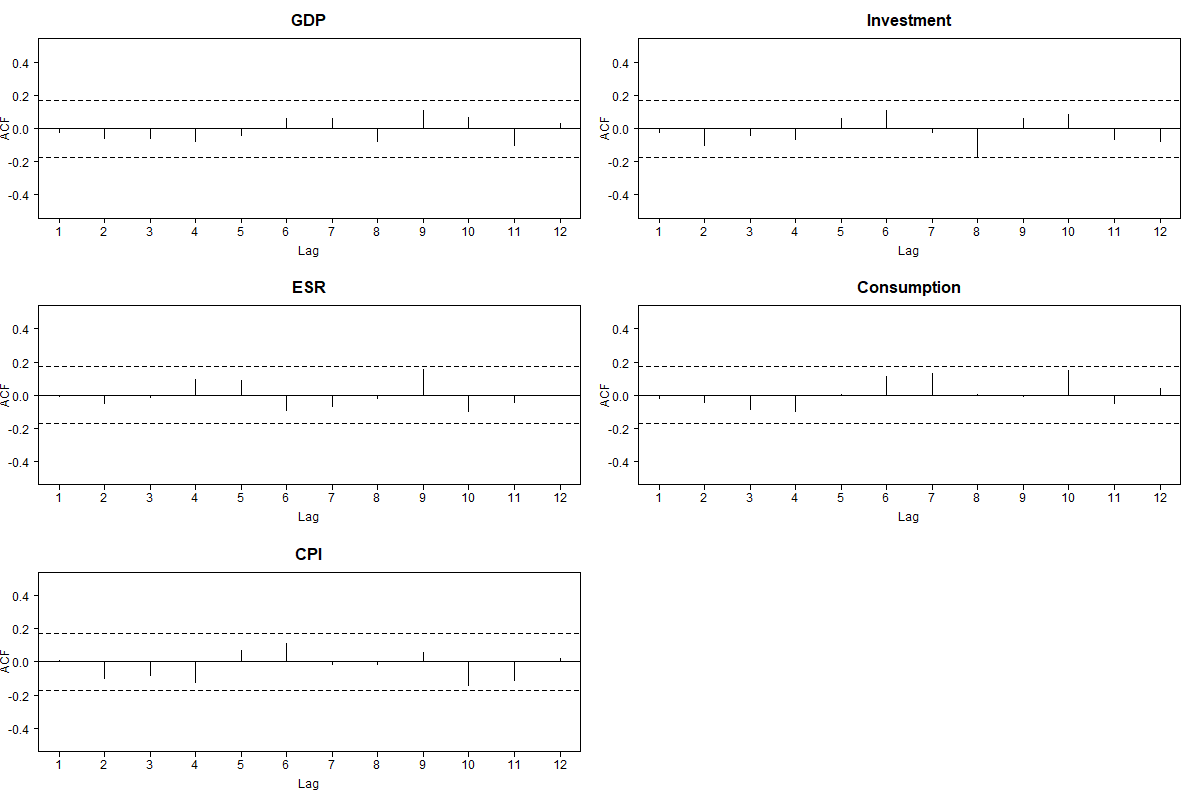
\includegraphics[width=1\textwidth,height=1\textheight,keepaspectratio]{acfplot.png}
	\caption{Autocorrelation for the VAR(3) model in log differences.}
	\label{fig:autocorr_diff}
\end{figure}



% The baseline forecasts in this case caputre all the realized values within their confidence intervals, except for the drop in consumption in the second quarter of 2014 discussed above.


\begin{figure}[ht]
	\centering
		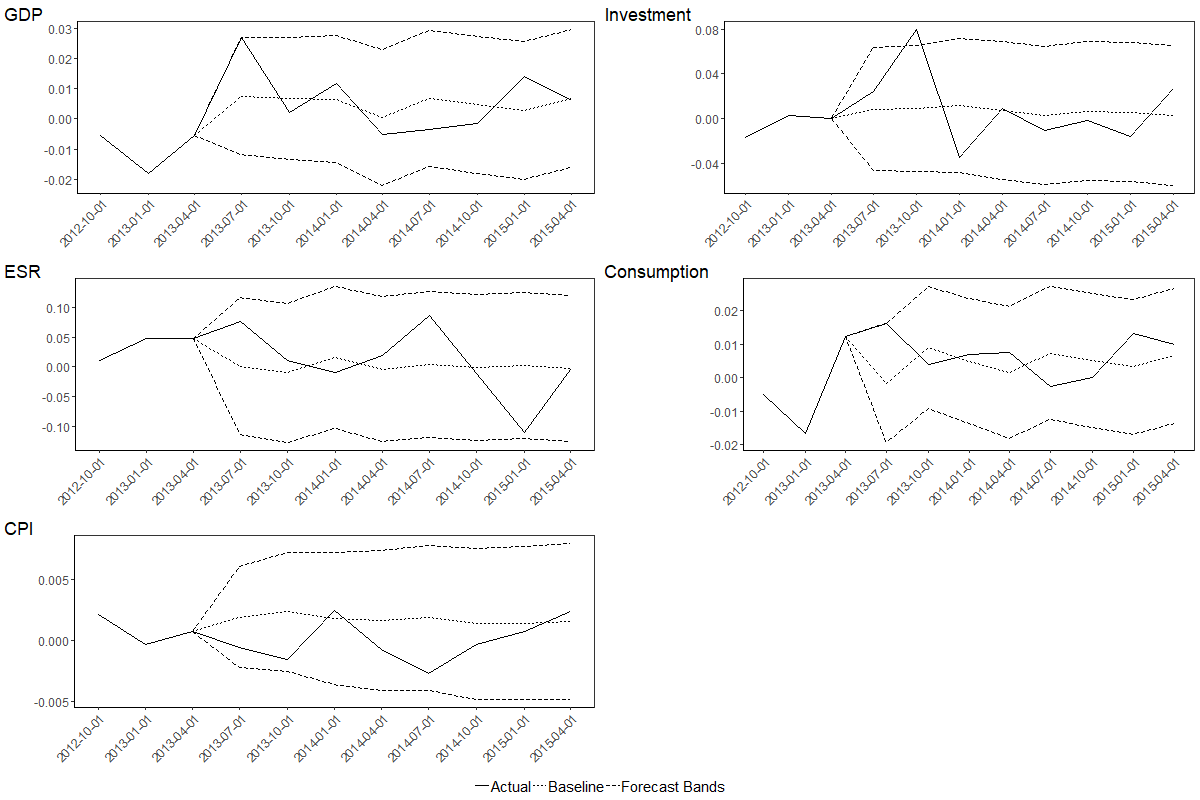
\includegraphics[width=1\textwidth,height=1\textheight,keepaspectratio]{basefcst.png}
	\caption{8-step forecasts for the baseline scenario.}
	\label{fig:baseline_comp_diff}
\end{figure}


\section{Results}



\subsection{Proportional Increase}
%\subsection{VAR(4) Model}
%
%Figure~\ref{fig:results_simplevar} shows the forecasts for the different scenarios in the case of the VAR(4) model in levels\footnote{[Review Comment:] Should I also report the confidence intervals (95\%) of the different forecasts here? Also, a more general question: The confidence intervals of the different forecasts overlap to some extent. The question now is what this tells me about the about the significance of the effects. If I run into problems here, I'd love some advice on how to deal with that problem.}. Table~\ref{tab:peak_simple} also shows the peak effects, which were calculated as the difference between the scenario forecast and the baseline forecast divided by the baseline value of the same period. As the forecasts originate from the same data in our presample period prior to 2013 Q2, the two scenarios differ only in their effect size, but not in their qualitative interpretation. Accordingly, replacing the increase in government spending by a decrease results in a mirrored image of the corresponding effects.
%
%For GDP, an increase in government spending causes an instant effect in the first period, which constitutes the peak impact of 1.30\% in the first scenario and 3.26\% in the second scenario. Sustaining these higher levels of spending, however, result in a slight decrease after one quarter and a reversal after the third quarter, where the values of GDP lie constantly below the baseline. Only after seven quarters, we can again observe a slight increase, but the original baseline levels are not reached in either scenario after two years.
%
%We can observe similar patterns for the excess stock returns of the construction sector and CPI inflation. Similarly to GDP, inflation increases after one quarter, reaching its peak effect of 0.16 percentage points in scenario 1 and 0.39 percentage points in scenario two. After five quarters, inflation falls below the baseline and stabilizes below the baseline. In the case of the excess stock returns, there is a longer lasting positive impact, and we reach a peak after one year of 18.12 percentage points and 45.30 percentage points respectively. Then, however, we find a reversal, where the excess stock returns decrease and fall below baseline levels after seven quarters. In contrast to GDP and inflation, excess stock returns also continue decreasing until the end of two years.
%
%Consumption and investment, on the other hand, exhibit clearer tendencies without a clear reversal within two years. Consumption increases from the first quarter onwards, reaching its peak effect of 1.47\% or 3.81\% after five quarters, and outperforms the baseline for the whole forecast period. The effects on investment, however, are even more pronounced. From the first period onwards, the increase in government spending leads to a drastic decrease of investment over the whole period, indicating a crowding out of private investment caused by the sustained higher levels of government spending. The peak effects on investment, indicating a decrease of 17.29\% and 43.22\% are the largest deviation from the baseline in our set of endogenous variables.
%
%
%
%\begin{figure}[ht]
%	\centering
%		\includegraphics[scale=0.55]{scenarios_simplevar_setting1.jpg}
%	\caption{Scenario forecasts for the VAR(4) model.}
%	\label{fig:results_simplevar}
%\end{figure}
%
%
%\begin{table}[ht]
%\centering
%%\begin{adjustbox}{width=1\textwidth}
%\begin{tabular}{|p{3cm}|p{1cm}|p{1.8cm}|p{1.6cm}|p{2.2cm}|p{1.6cm}|}
%\hline
%  & GDP    & Investment & Excess Stock Returns &	Consumption & CPI Inflation \\ \hline \hline
%Scenario 1 - +10 \%                   & 1.30\% & -17.29\%   & 18.12 pp             & 1.47\%      & 0.16 pp       \\
%\hline
%Scenario 2 - +25 \%                   & 3.26\% & -43.22\%   & 45.30 pp             & 3.81\%      & 0.39 pp    \\
%\hline  
%\end{tabular}
%
%%\end{adjustbox}
%\caption{Peak Effects in the VAR(4) forecasts.}
%\label{tab:peak_simple}
%\end{table}

%\subsection{dVAR(3) Model}


As Table~\ref{tab:wtest} shows for the shift in government spending, only the policy forecasts for GDP and Consumption growth differ significantly from the baseline forecast. We would hence conclude, that, in the median, a constant increase in government spending only has a significant effect on those two variables. The 8-step forecasts estimated for all series from the model can be seen in Figure~\ref{fig:results_dvar}. These results described above persist en gros after increasing the number of exogenous lags in government expenditure, except for a significant - but nonetheless similarly small - effect size on CPI for $q \geq 3$. 

For GDP growth, the increase in government spending in the second quarter of 2013 let to an instant shift in both scenarios. Thereafter, the paths for the counterfactual scenarios are simply shifted and diverge increasingly with time. In any case, however, both the difference between the scenarios and the speed of their divergence are very small with a peak effect of 0.05 percentage points in 2015 Q2 for Scenario 1, and a peak effect of 0.13 percentage points for Scenario 2 in 2015 Q2. The growth paths for consumption develop in a similar fashion as for GDP. In both scenarios, the forecasts stay relatively close to the baseline and then reach their respective peak effects at the end of the forecast horizon at 0.05 percentage points and 0.12 percentage points in 2015 Q2.

Given the relatively strong assumption of the policy scenarios, in which the policymakers could raise government spending 10\% and 25\% higher than they actually did, the effects of the policy change are surprisingly small. Even more so, as the effect seemed to not manifest itself across all the variables we were considering in this exercise.

\begin{figure}[!htbp]
	\centering
	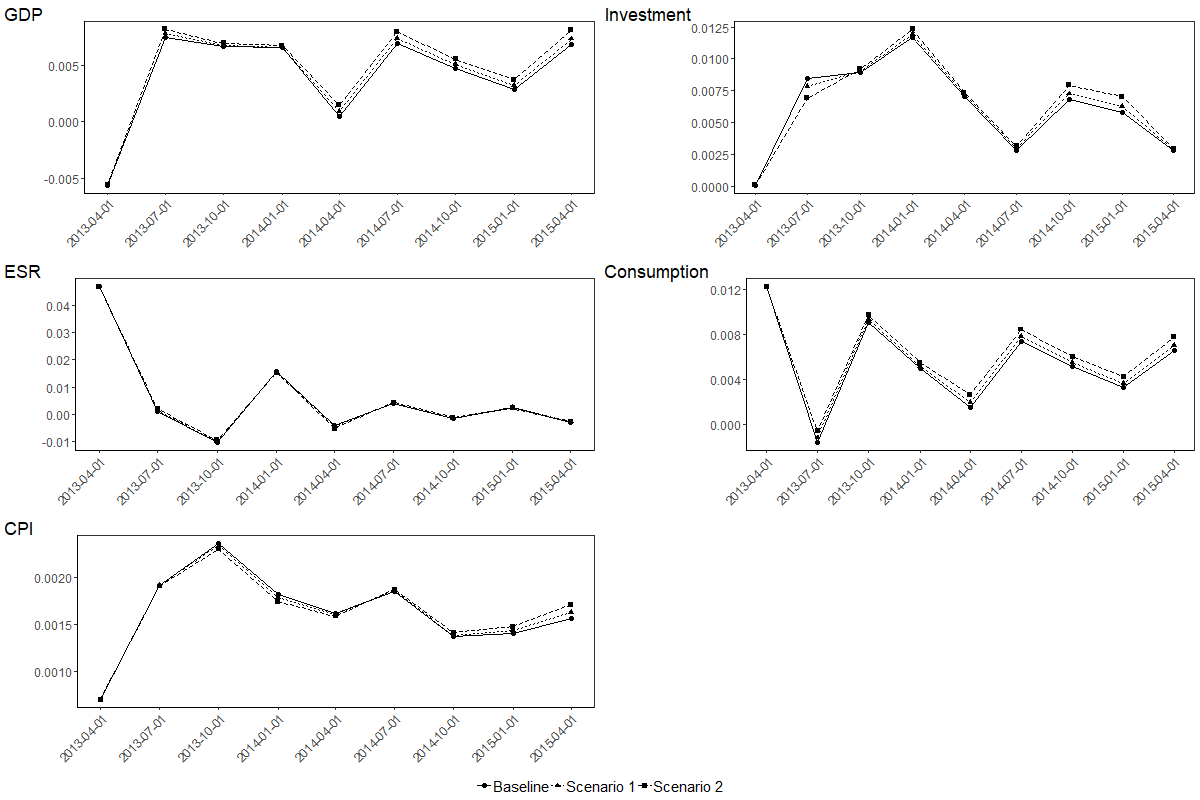
\includegraphics[width=1\textwidth,height=1\textheight,keepaspectratio]{scenariofcst.png}
	\caption{Forecasts for the policy scenarios with a proportional increase over the forecast horizon.}
	\label{fig:results_dvar}
\end{figure} 

\begin{table}[!htbp] \centering 
	\caption{Peak effects and results of Wilcoxon Signed Rank test for the scenarios vs. baseline for a proportional increase over the forecast horizon} 
	\label{tab:wtest} 
	\begin{tabular}{@{\extracolsep{5pt}} lrrrr} 
		\\[-1.8ex]\hline 
		\hline \\[-1.8ex]
		& Peak Effect 10\% & Peak Effect 25\% & Test Statistic & p \\ 
		\hline \\[-1.8ex] 
		GDP & $0.05$ p.p. & $0.13$ p.p. & $0$ & $0.01$ \\ 
		Investment & $-0.06$ p.p. & $-0.15$ p.p. & $8$ & $0.20$ \\ 
		ESR & $0.05$ p.p. & $0.12$ p.p. & $16$ & $0.84$ \\ 
		Consumption & $0.05$ p.p. & $0.12$ p.p. & $0$ & $0.01$ \\ 
		CPI & $0.006$ p.p. & $0.01$ p.p. & $16$ & $0.84$ \\ 
		\hline \\[-1.8ex] 
	\end{tabular} 
\end{table}  

%\begin{table}[!htbp] \centering 
%	\caption{Jarque-Bera Test Statistics for the dVar(3) Model} 
%	\label{tab:jbtest} 
%	\begin{tabular}{@{\extracolsep{5pt}} cc} 
%		\\[-1.8ex]\hline 
%		\hline \\[-1.8ex] 
%		Statistic & p  \\ 
%		\hline \\[-1.8ex] 
%		$94.2727$ & $0.000$ \\ 
%		\hline \\[-1.8ex] 
%	\end{tabular} 
%\end{table}


\subsection{Constant Increase}

Figure~\ref{fig:results_dvarL} shows the forecasts with a constant increase in government spending in each period of the forecast horizon. Notably, the differences in the growth paths of the variables between the baseline forecast and the alternative policy scenarios are more pronounced than during a period of proportionally increased government spending. For GDP and ESR and consumption the forecasts indicate an increase in growth right from the beginning, followed by a decrease below baseline levels and consequent convergence where consumption growth converges the latest toward the baseline. The deviations are more pronounced for Scenario 2 than they are for Scenario 1. Investment growth exhibits fluctuations in the opposite direction as the other variables.. The only statistically significant effect after the increase is seen in inflation, reaching its peak effects 0.62 and 1.54 percentage points in the respective scenario. It is also the only variable that still shows a relatively clear difference between the scenarios and the baseline at the end of the forecast horizon.

Although the total size of the increase over the forecast horizon is the same as for the proportional spending increase, the effects exhibited in the forecasts, both in terms of behavior over time and statistical significance are quite different. The differences in the variables other than inflation seem to whither away over time, leaving the economy with temporarily increased inflation, which is also drifting back to its pre-policy levels. 

\begin{figure}[!htbp]
	\centering
	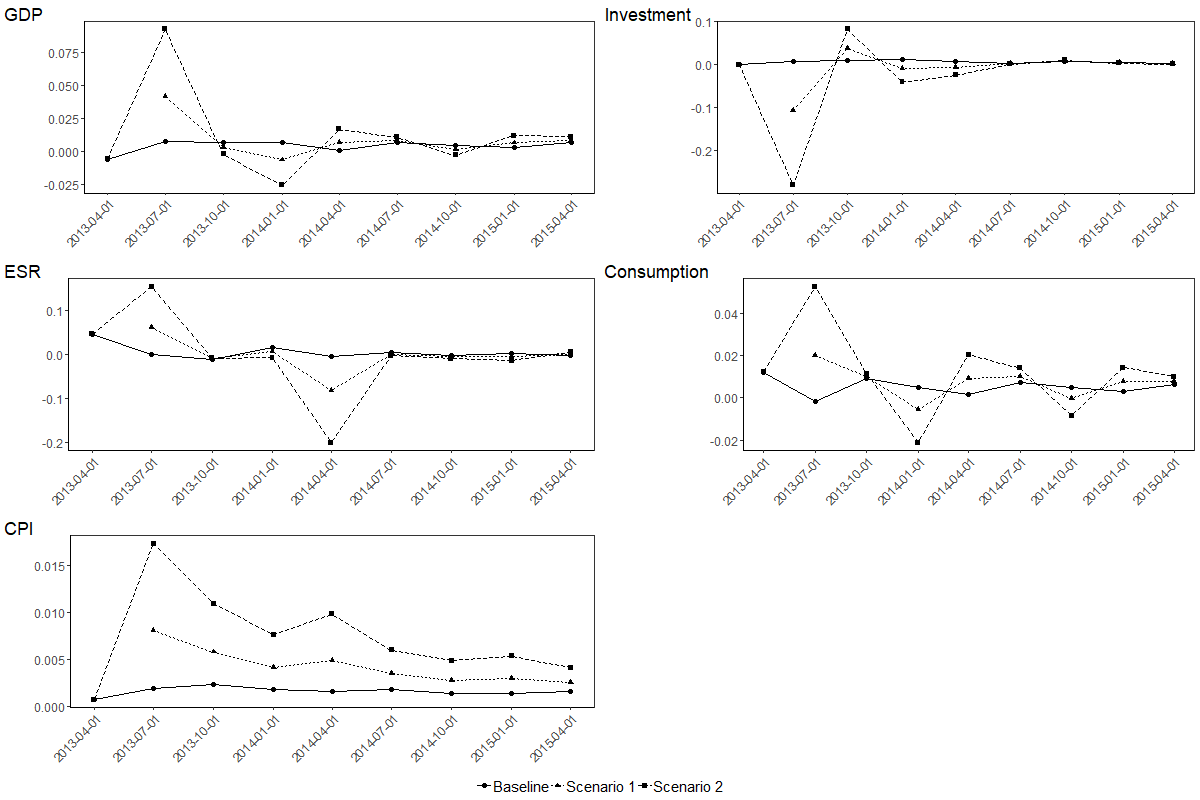
\includegraphics[width=1\textwidth,height=1\textheight,keepaspectratio]{scenariofcst_linear.png}
	\caption{Forecasts for the policy scenarios for a constant increase over the forecast horizon.}
	\label{fig:results_dvarL}
\end{figure} 

\begin{table}[!htbp] \centering 
	\caption{Peak effects and results of Wilcoxon signed-rank test of the scenarios vs baseline for a constant increase over the forecast horizon.} 
	\label{tab:wtestL} 
	\begin{tabular}{@{\extracolsep{5pt}} lrrrr} 
		\\[-1.8ex]\hline 
		\hline \\[-1.8ex]
		& Peak Effect 10\% & Peak Effect 25\% & Test Statistic & p \\ 
		\hline \\[-1.8ex] 
		\hline \\[-1.8ex] 
		GDP & $3.40$ p.p. & $8.50$ p.p. & $14$ & $0.64$ \\ 
		Investment & $-11.58$ p.p. & $-28.95$ p.p. & $25$ & $0.38$ \\ 
		ESR & $-7.84$ p.p. & $-19.60$ p.p. & $24$ & $0.46$ \\ 
		Consumption & $2.18$ p.p. & $5.46$ p.p. & $12$ & $0.46$ \\ 
		CPI & $0.62$ p.p. & $1.54$ p.p. & $0$ & $0.01$ \\ 
		\hline \\[-1.8ex] 
	\end{tabular} 
\end{table}  

\subsection{One-Time Increase with Instant "Payback"}

Directionally, the responses in GDP and investment growth after a unique increase of government spending in the first quarter of the forecast horizon are similar to the responses after a constant spending increase, albeit with their peaks shifted to the first quarter after the increase happens. Consumption growth also shows a pattern of fluctuation similar to the one in the constant spending increase scenario. ESR growth fluctuates away from the baseline much more clearly in this scenario than before, falling beneath base levels six months after the increase and remains lower than the baseline until it recovers and then comes back to baseline levels. Inflation is - like the other variables - also not significantly affected by the policy measure, converging to the baseline quickly. The effects remain unsignificant even after doubling the increases in the respective scenarios, indicating that the effects of one-off increases in government expenditure are rather scale-insensitive and do not affect the growth paths of the variables in question.

\begin{figure}[!htbp]
	\centering
	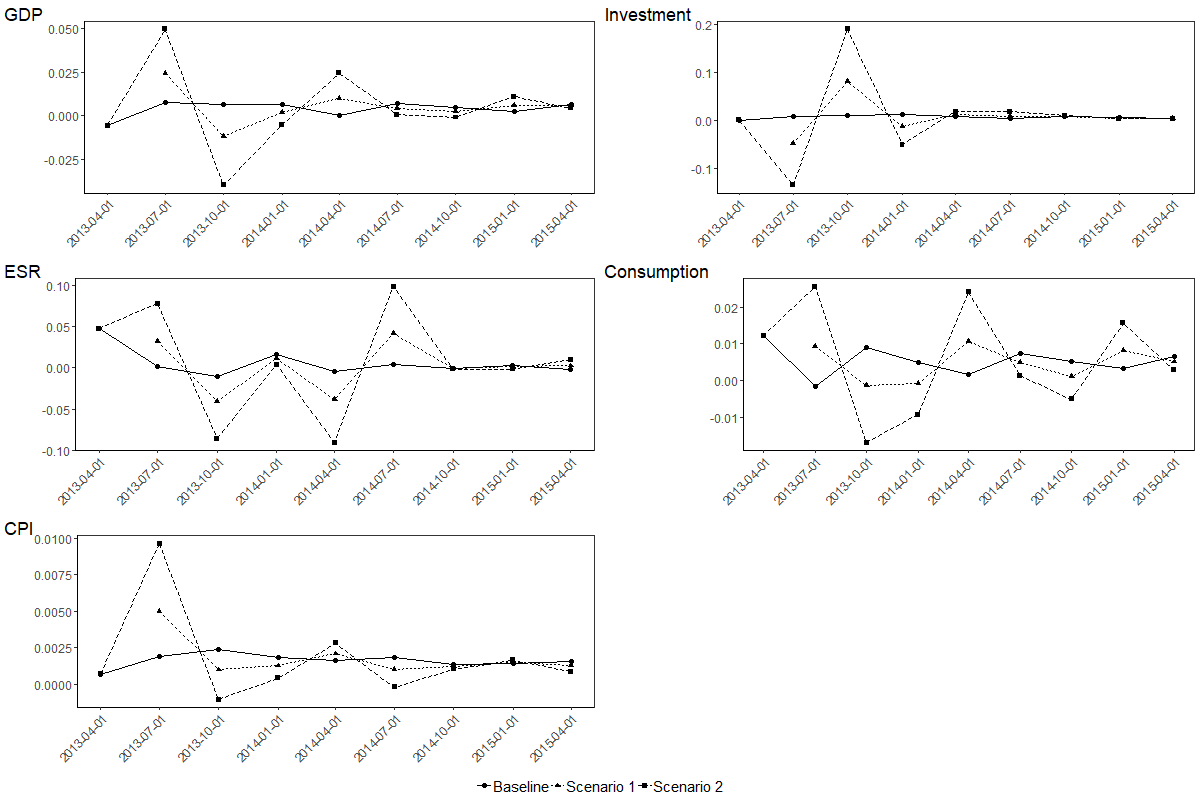
\includegraphics[width=1\textwidth,height=1\textheight,keepaspectratio]{scenariofcst_OneTime.png}
	\caption{Peak effects and results of Wilcoxon signed-rank test of the scenarios vs baseline for a one-time increase.}
	\label{fig:results_dvarOT}
\end{figure} 

\begin{table}[!htbp] \centering 
	\caption{Results of Wilcoxon Signed Rank test for Scenarios vs Baseline for a one-time increase.} 
	\label{tab:wtestOT} 
	\begin{tabular}{@{\extracolsep{5pt}} lrrrr} 
		\\[-1.8ex]\hline 
		\hline \\[-1.8ex]
		& Peak Effect 10\% & Peak Effect 25\% & Test Statistic & p \\ 
		\hline \\[-1.8ex] 
	\hline \\[-1.8ex] 
	GDP & $-1.86$ p.p. & $-4.66$ p.p. & $19$ & $0.95$ \\ 
	Investment & $7.26$ p.p & $18.07$ p.p. & $16$ & $0.84$ \\ 
	ESR & $3.76$ p.p. & $9.41$ p.p. & $18$ & $1.00$ \\ 
	Consumption & $1.09$ p.p. & $2.72$ p.p. & $18$ & $1.00$ \\ 
	CPI & $0.31$ p.p. & $0.77$ p.p. & $23$ & $0.55$ \\ 
	\hline \\[-1.8ex] 
	\end{tabular} 
\end{table}  


%The effect sizes are similarly small for investment growth, but the behavior of the growth paths, is more interesting. In the first period, the increase in government spending seems to slightly slow down investment growth. The picture reverts, however, as in both scenarios investment growths jumps ahead of the baseline from the second quarter after the increase onwards. Both scenarios again reach their peak effect at the same time in the first quarter of 2015 with 0.04 percentage points in Scenario 1 and 0.12 percentage points in Scenario 2. In the last period, all forecasts converge again.



%The effects of an increase in government spending on the growth path of GDP are less straightforward than the level effects we obtained from the VAR(4) model. Upon increasing government expenditure, GDP growth reaches a peak effect of 1.59 percentage points in the first, and 3.98 percentage points in the second scenario. After that, however, the sustained levels of government expenditure cause GDP growth to fall below the baseline in the second and third quarter, after which it returns to a similar growth path as in the baseline scenario. In our forecasts we can observe similar patterns for the growth paths of investment and consumption. The growth of consumption increases in the first quarter by 0.98 or 2.44 percentage points, respectively, after which it fluctuates around the growth path of the baseline prediction. Furthermore, the higher levels of government expenditure seem to intensify the volatility of consumption growth. For investment growth, the increase in government expenditure here also has a negative effect. It is, however, less persisting than in the VAR(4), case. Right after the increase of government expenditure, the growth rate for investment drops by 5.87 percentage points in scenario 1 and 14.68 percentage points in scenario two. Then, however, the growth rate stabilizes around the baseline after five quarters, indicating quite a different effect in levels compared to the VAR(4) model.
%
%Similarly interesting are the effects of the increase in government spending on excess stock returns and CPI inflation. As mentioned above, these time series were not modified for the dVAR(3) model, as they were already expressed as logarithmic differences. The implications of the dVar model, however, seem to have quite different implications on these series. In the case of the excess stock returns, the increase in government expenditure causes them to increase for the first three quarters by up to 9.96 percentage points and 24.91 percentage points. Then, after the third quarter, they approach the levels of the baseline forecast without reaching them within two years, however. In the first quarter, CPI inflation also increases by 0.29 percentage points in scenario 1 and 0.72 percentage points in scenario 2. Subsequently, they close in to the baseline forecast at a slower rate than the excess stock returns of the construction sector



%\begin{table}[ht]
%\centering
%%\begin{adjustbox}{width=1\textwidth}
%\label{tab:peak_dvar}
%\begin{tabular}{|p{3cm}|p{1cm}|p{1.8cm}|p{1.6cm}|p{2.2cm}|p{1.6cm}|}
%\hline
%  & GDP    & Investment & Excess Stock Returns & Consumption & CPI Inflation \\ \hline \hline
%Scenario 1 - +10 \%                   & 1.59 pp & -5.87 pp   & 9.96 pp             & 0.98 pp      & 0.29 pp       \\
%\hline
%Scenario 2 - +25 \%                   & 3.98 pp & -14.68 pp   & 24.91 pp             & 2.44 pp      & 0.72 pp    \\
%\hline  
%\end{tabular}
%%\end{adjustbox}
%\caption{Peak Effects in the dVAR(3) forecasts.}
%\end{table}
%Put into Conclusion
%Considering the effects in levels, it seems questionable whether sustaining such, admittedly, extreme increases in government spending over an extended period of time is a sustainable option for policy makers.




\subsection{One-Time Increase with Gradual "Payback"}

The effects of government spending being gradually reduced after a one-time increase can be seen in Figure~\ref{fig:results_dvarLR}. Qualitatively, they are closer to the proportional spending increase than to the one-time measure followed by an instant reduction of government spending. All growth variables converge to the baseline by the end of the forecast horizon and end up close to pre-policy rates. However, in contrast to the proportional spending increase, none of the growth paths were significantly impacted by the spending increase, indicating that in the short term, it does not make a difference for the growth paths of the endogenous variables whether the government immediately returns to reduced spending or gradually reduces it over time.

\begin{figure}[!htbp]
	\centering
	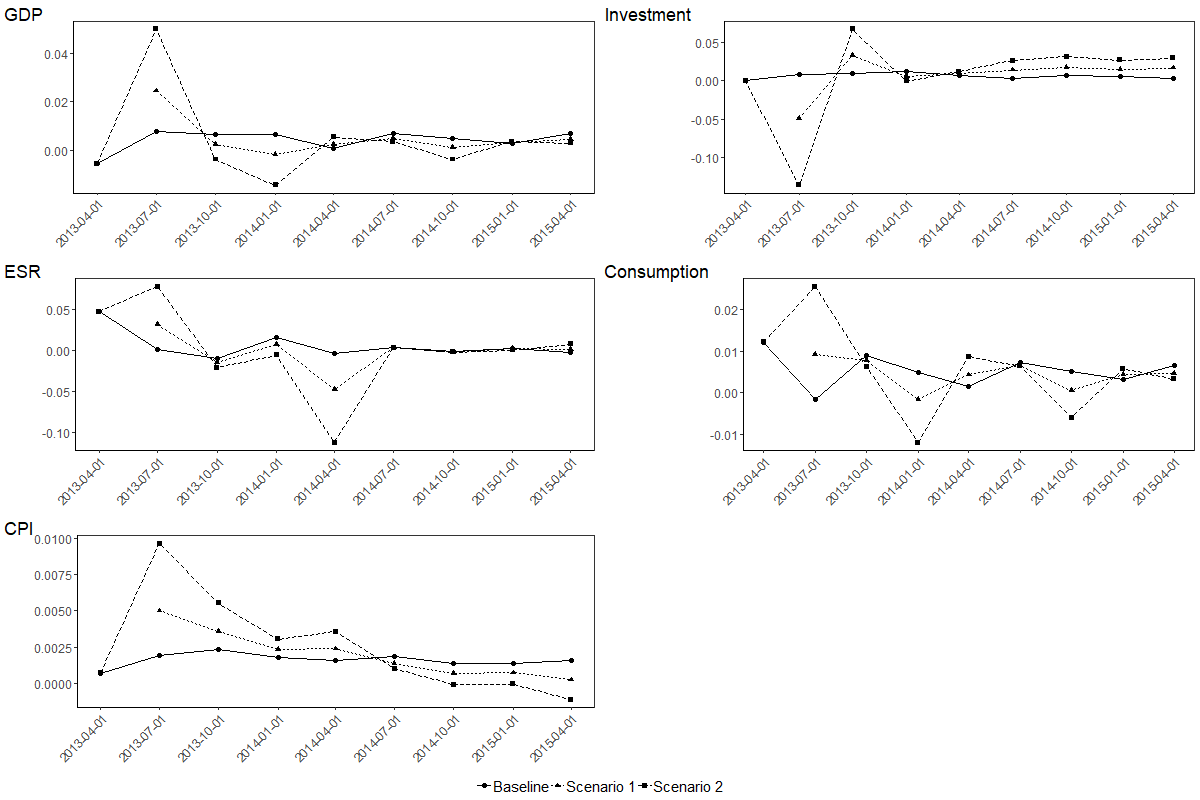
\includegraphics[width=1\textwidth,height=1\textheight,keepaspectratio]{scenariofcst_linearred.png}
	\caption{Forecasts for the policy scenarios for a one-time increase with subsequent gradual reduction.}
	\label{fig:results_dvarLR}
\end{figure} 

\begin{table}[!htbp] \centering 
	\caption{Peak effects and results of Wilcoxon signed-rank test of the scenarios vs baseline for a one-time increase with subsequent gradual reduction.} 
	\label{tab:wtestLR} 
	\begin{tabular}{@{\extracolsep{5pt}} lrrrr} 
		\\[-1.8ex]\hline 
		\hline \\[-1.8ex]
		& Peak Effect 10\% & Peak Effect 25\% & Test Statistic & p \\ 
		\hline \\[-1.8ex] 
		\hline \\[-1.8ex] 
		GDP & $1.69$ p.p. & $4.23$ p.p. & $25$ & $0.38$ \\ 
		Investment & $-5.77$ p.p. & $-14.41$ p.p. & $10$ & $0.31$ \\ 
		ESR & $-4.32$ p.p. & $-10.75$ p.p. & $25$ & $0.38$ \\ 
		Consumption & $-1.09$ p.p. & $2.72$ p.p. & $21$ & $0.74$ \\ 
		CPI & $0.31$ p.p. & $0.77$ p.p. & $15$ & $0.74$ \\ 
		\hline \\[-1.8ex] 
	\end{tabular} 
\end{table}  
\section{Discussion of the Results and Conclusion}

The results of the counterfactual scenarios allow two main conclusions. First, they indicate that the effects of government spending increases depend on how these spendings are made. In the median, one-time increases fail to significantly alter the growth paths of the macroeconomic variables we included over a period of two years, regardless of whether spending returns to lower levels instantly or is reduced gradually over the subsequent quarters.

Continually sustained increases in government spending, on the other, seem to have a significant positive impact on GDP and consumption growth if they are implemented as a proportional 'markup' on actual expenditure, and a significant positive effect on inflation if the same increase is spread in constant rates over each quarter. Still, these effects were small, especially when they are held against the direct economic costs and the political feasibility to increase government expenditure so drastically from one quarter to another. 

Nonetheless, it is important to keep in mind that the forecast methodology was rather simple and is easily extensible. It imposed little structure on the data, other than the choice of variables and their ordering -- modeling decisions that are difficult to avoid, but can be tested for -- the exogeneity of government expenditure as a fiscal policy instrument, which can be avoided by, for example, by finding and employing appropriate instrumental, that are indeed exogenous. Finding such instruments can also help determine, to which extent governments are free in their fiscal policy choice and is an exercise which can also be primarily data-driven by employing exogeneity employing tests for exogeneity, such as the one proposed by \citet{ericsson1998}, who examined necessary conditions for exogeneity of variables. Another implicit assumption of this model is the time- and policy-insensitive behavior of economic agents. This is reflected in the constant coefficients of the model, which impose the lack of regime changes over a time frame of 35 years. Without imposing any more structure, endogenous regime changes can also be estimated from the underlying data, as in \citet{kim2008}. Employing approaches similar to this exercises could thus help to motivate deeper research into estimated relationships, using larger datasets, or employing more flexible methods, such as the Large Bayesian VAR model employed by \citeauthor{kapetanios2012}.

Similar approaches could also be taken for policy evaluation and forecasting in scenarios, where good forecasts are more important than identifying economic relationships. Employing methods from machine learning can help to tune VAR models to produce good forecasts in situations, when sufficient data is available, or when bootstrapping or other data augmentation methods are available. The approach itself can thus be of interest for aims other than economic research, regardless of whether it is in the context of fiscal policy or other macroeconomic policy measures.


%adopt style
\bibliographystyle{dcu}
\bibliography{Sources}

\pagebreak
\appendix
\section{Source Code for Analysis}
The following listings can be found on \href{https://github.com/kaiharuto/masterthesis}{GitHub} 


\lstinputlisting[breaklines=true, language=R, caption=Analysis.R, frame = single]{Analysis.R}
\lstinputlisting[breaklines=true, language=R, caption=utilityfunc.R, frame = single]{utilityfunc.R}

\end{document}
